\documentclass[11pt]{aghdpl}
% \documentclass[en,11pt]{aghdpl}  % praca w języku angielskim
\usepackage{lipsum}
% Lista wszystkich języków stanowiących języki pozycji bibliograficznych użytych w pracy.
% (Zgodnie z zasadami tworzenia bibliografii każda pozycja powinna zostać utworzona zgodnie z zasadami języka, w którym dana publikacja została napisana.)
\usepackage[english,polish]{babel}

% Użyj polskiego łamania wyrazów (zamiast domyślnego angielskiego).
\usepackage{polski}

\usepackage[utf8]{inputenc}

% dodatkowe pakiety
\usepackage{url}
\usepackage{mathtools}
\usepackage{amsfonts}
\usepackage{amsmath}
\usepackage{amsthm}

% --- < bibliografia > ---

\usepackage[
style=numeric,
sorting=none,
%
% Zastosuj styl wpisu bibliograficznego właściwy językowi publikacji.
language=autobib,
autolang=other,
% Zapisuj datę dostępu do strony WWW w formacie RRRR-MM-DD.
urldate=iso8601,
% Nie dodawaj numerów stron, na których występuje cytowanie.
backref=false,
% Podawaj ISBN.
isbn=true,
% Nie podawaj URL-i, o ile nie jest to konieczne.
url=false,
%
% Ustawienia związane z polskimi normami dla bibliografii.
maxbibnames=3,
% Jeżeli używamy BibTeXa:
backend=bibtex
]{biblatex}

\usepackage{csquotes}
% Ponieważ `csquotes` nie posiada polskiego stylu, można skorzystać z mocno zbliżonego stylu chorwackiego.
\DeclareQuoteAlias{croatian}{polish}

\addbibresource{bibliografia.bib}

% Nie wyświetlaj wybranych pól.
%\AtEveryBibitem{\clearfield{note}}


% ------------------------
% --- < listingi > ---

% Użyj czcionki kroju Courier.
\usepackage{courier}

\usepackage{listings}
\lstset{escapeinside={(*@}{@*)}}

\usepackage[toc,page]{appendix}

\usepackage[hidelinks]{hyperref}

\lstloadlanguages{TeX}

\lstset{
	literate={ą}{{\k{a}}}1
           {ć}{{\'c}}1
           {ę}{{\k{e}}}1
           {ó}{{\'o}}1
           {ń}{{\'n}}1
           {ł}{{\l{}}}1
           {ś}{{\'s}}1
           {ź}{{\'z}}1
           {ż}{{\.z}}1
           {Ą}{{\k{A}}}1
           {Ć}{{\'C}}1
           {Ę}{{\k{E}}}1
           {Ó}{{\'O}}1
           {Ń}{{\'N}}1
           {Ł}{{\L{}}}1
           {Ś}{{\'S}}1
           {Ź}{{\'Z}}1
           {Ż}{{\.Z}}1,
	basicstyle=\footnotesize\ttfamily,
}

% ------------------------

\AtBeginDocument{
	\renewcommand{\tablename}{Tabela}
	\renewcommand{\figurename}{Rys.}
}

% ------------------------
% --- < tabele > ---

\usepackage{array}
\usepackage{tabularx}
\usepackage{multirow}
\usepackage{booktabs}
\usepackage{makecell}
\usepackage[flushleft]{threeparttable}

% defines the X column to use m (\parbox[c]) instead of p (`parbox[t]`)
\newcolumntype{C}[1]{>{\hsize=#1\hsize\centering\arraybackslash}X}

%---------------------------------------------------------------------------

\author{Wojciech Gumuła}
\shortauthor{W. Gumuła}

%\titlePL{Przygotowanie bardzo długiej i pasjonującej pracy dyplomowej w~systemie~\LaTeX}
%\titleEN{Preparation of a very long and fascinating bachelor or master thesis in \LaTeX}

\titlePL{Wykorzystanie systemu operacyjnego Linux we wbudowanych systemach wizyjnych zrealizowanych na platformie Zynq.}
\titleEN{The use of the Linux operating system in embedded vision systems implemented on the Zynq platform.}


\shorttitlePL{System operacyjny Linux na platformie Zynq.} % skrócona wersja tytułu jeśli jest bardzo długi
\shorttitleEN{Linux OS on the Zynq platform.}

\thesistype{Praca dyplomowa magisterska}
%\thesistype{Master of Science Thesis}

\supervisor{dr Tomasz Kryjak}
%\supervisor{Marcin Szpyrka PhD, DSc}

\degreeprogramme{Automatyka i Robotyka}
%\degreeprogramme{Computer Science}

\date{2017}

\department{Katedra Automatyki i Inżynierii Biomedycznej }
%\department{Department of Applied Computer Science}

\faculty{Wydział Elektrotechniki, Automatyki,\protect\\[-1mm] Informatyki i Inżynierii Biomedycznej}
%\faculty{Faculty of Electrical Engineering, Automatics, Computer Science and Biomedical Engineering}

\acknowledgements{Serdecznie dziękuję Adamie Giży za bycie Giżą.}


\setlength{\cftsecnumwidth}{10mm}

%---------------------------------------------------------------------------
\setcounter{secnumdepth}{4}
\brokenpenalty=10000\relax

\begin{document}

\titlepages

\fancypagestyle{plain}
{
	% Usuń nagłówek i stopkę
	\fancyhf{}
	% Usuń linie.
	\renewcommand{\headrulewidth}{0pt}
	\renewcommand{\footrulewidth}{0pt}
}

\setcounter{tocdepth}{2}
\tableofcontents
\clearpage

\chapter{Wstęp}
\label{cha:intruduction}

%TODO Przed tym dodać abstrakt PL i EN (na jednej stronie)

Przetwarzanie obrazów i ich sekwencji stanowi pole rozległych badań naukowych i przemysłowych. %TODO naukowych i przemysłowych 
% OK

W ich ramach, projektowane są algorytmy umożliwiające akwizycję, modyfikowanie, analizę, rozpoznawanie treści i prezentację obrazów. %TODO jeszcze rozpoznawanie treści
% OK
Często motywacją badań jest próba naśladowania zjawisk związanych z narządem wzroku człowieka i dążenie do uzyskania takiego opisu sposobu działania, aby umożliwić wykonanie zbliżonego do nich algorytmu przy użyciu układów elektronicznych. %TODO zjawisk -> sposobu działania, drugie zjawisk jest jakieś zbyt ogólne
% OK
Odmiennym zagadnieniem jest poszukiwanie możliwości realizacji przetwarzania obrazów w taki sposób, aby uzyskać informacje niewidoczne dla ludzkiego oka, w oparciu o parametry obrazu o niewielkiej zmienności. Temat ten obejmuje analizę obrazów w celu wykrycia możliwych modyfikacji obrazu oryginalnego czy algorytmy częstotliwościowe. %TODO tu mógłby Pan rozwinąć, co ma Pan na myśli...
% OK

Techniki przetwarzania obrazów opierają się zwykle na analizie i redukcji informacji zawartej w sekwencji pikseli w taki sposób, aby uzyskać obraz wynikowy, na którym uwypuklone będą kluczowe z punktu widzenia algorytmu własności. %TODO informacji zawartej w sekwencji.. 
% OK
Wynikiem działania procedury może być również zbiór cech opisujących badane zjawiska.
%TODO W tym miejscu bym przytoczył klasyczny podział na przetwarzanie, analizę i rozpoznawanie i krótko omówił...
% OK

Zdefiniować można szereg operacji składających się na proces przetwarzania obrazu \cite{Tadeusiewicz1997}.
\begin{itemize}
	\item Akwizycja -- przygotowanie cyfrowej reprezentacji obrazu, czytelnej dla układu obliczeniowego.
	
	\item Przetwarzanie -- proces modyfikacji danych wejściowych w celu przystosowania do obróbki algorytmicznej. Wykorzystujący, między innymi, operacje skalowania, zmiany przestrzeni barw czy usuwania zakłóceń.
	
	\item Analiza -- redukcja informacji wizyjnej w celu uzyskania opisu jakościowego lub ilościowego badanych cech i eliminacja zbędnych z perspektywy rozpatrywanego zadania informacji.
	
	\item Rozpoznawanie -- proces uzyskiwania informacji wynikowych na podstawie wektora cech.
\end{itemize}

Techniki przetwarzania obrazów, a zwłaszcza ich sekwencji znajdują zastosowanie w coraz większej liczbie dziedzin. %TODO przypadków -> złe słowo.
% OK?
Jedną z dziedzin wykorzystujących techniki wizyjne, która jest prężnie rozwijana w ostatnich latach jest budowa systemów ADAS (\emph{ang.} Advanced driver-assistance systems). %TODO ulega rozwojowi -> średnie...
% OK?
Ich działanie, poza sygnałami wizyjnymi, wymaga użycia sygnałów o innych charakterystykach, między innymi czujników optycznych oraz systemów \emph{LIDAR}.
Celem projektowania zaawansowanych systemów wsparcia kierowcy jest stopniowe zwiększanie autonomii pojazdów i ograniczenie zaangażowania kierowcy. W szerszej perspektywie, rozwój systemów ADAS może pozwolić na zaprojektowanie pojazdów w pełni autonomicznych, pozwalających na transport osób i towarów bez udziału kierowców.
Dane z czujników wizyjne mogą być przetwarzane w celu uzyskania informacji na temat jezdni, innych uczestników ruchu, oznakowania czy potencjalnych zagrożeń. 
Opracowanie współcześnie stosowanych technik znaleźć można w pracach \cite{Bengler2014,Velez2017}.
%TODO OK, choć kilka zdań więcej też by można. 1. Wprost nazwać co wchodzi w skład ADAS (jakie podsystemy) 2. Coś o pojazdach autonomicznych.,
% OK

Inny zbiór technik wykorzystywany jest w celu detekcji i rozpoznawania twarzy oraz badania emocji. %TODO może jeszcze detekcji twarzy.
% OK
Zagadnienie to znajduje zastosowanie w ramach projektowania nie tylko systemów przemysłowych, ale jest również powszechnie stosowane w oprogramowaniu współcześnie dostępnych aparatów cyfrowych czy w ramach serwisów społecznościowych. Metody te mogą również pozwolić na budowę systemów weryfikacji użytkownika bez konieczności zdefiniowania hasła dostępu. Znajdują także zastosowanie w interfejsach przystosowanych do pracy z osobami niepełnosprawnymi.
Analizę wykorzystywanych w tym celu algorytmów znaleźć można w pracy \cite{Anil2016}.
%TODO też nieco szerzej o tych aplikacjach
% OK

Współcześnie, coraz większe znaczenie mają również systemy śledzenia osób i analizy ich zachowań w celu wykrycia zachowań niepożądanych. %TODO przechodniów -> osób. działań -> zachowań
% OK
Motywując to zwiększeniem bezpieczeństwa, badane są takie zagadnienia jak detekcja porzuconych bagaży, obecność osób nieuprawnionych w ustalonych strefach czy śledzenie ruchu i reidentyfikacja przy użyciu wielu kamer. %TODO jeszcze re-identyfikacja
% OK
Potrzeba automatyzacji wynika ze złożoności projektowanych systemów, które zasięgiem obejmować mogą całe aglomeracje i pozwalać na obserwację zachować tysięcy osób. Z tego powodu, praktycznie niemożliwe jest zapewnienie liczby operatorów pozwalającej na wykorzystanie informacji wejściowych w pełni.
Systemy te mogą działać niezależnie lub stanowić jeden z elementów zintegrowanego oprogramowania, wykorzystującego dane z wielu źródeł \cite{Sriram2016,Hussain2016,Gouo2015}.
%TODO O tym monitoringu też 2 zdania więcej. Przede wszystkim z czego wynika potrzeba automatyzacji.
% OK

Równolegle do rozwoju algorytmów wizyjnych, badane są techniki implementacji pozwalających na wykorzystanie ich w systemach uruchamianych na układach elektronicznych różnego typu. %TODO rzeczywistych -> a co te algorytmy na wirutalnych są rozwijane. Tzw. wiem o co Panu chodzi, ale zły dobór słów.
% OK?
Algorytmy wizyjne projektowane są z myślą o uruchamianiu na powszechnie stosowanych układach procesorowych w architekturach x86 lub ARM, mikrokontrolerach, układach ASIC (\emph{ang.} Application Specific Integrated Circuit) i FPGA (\emph{ang.} Field-Programmable Gate Array). %TODO rozwinąć skróty
% OK

Pośród wymienionych platform wyróżnić można rodzinę Zynq \cite{zybo-reference-manual}, integrującą możliwości układów FPGA oraz procesorów ARM. 
Dzięki zastosowaniu logiki programowalnej, możliwe jest projektowanie algorytmów wizyjnych wykonywanych w sposób strumieniowy, zapewniając wysoką wydajność przy stosunkowo niskim zapotrzebowaniu na energię. %TODO może logiki programowalnej...
% OK
Uzupełnieniem takiego układu jest procesor ARM, umożliwiający wykorzystanie algorytmów, które wymagają swobodnego dostępu do kontekstu obliczeniowego. Procesor sekwencyjny jest również, w porównaniu do układów logicznych, lepiej przystosowany do wykonywania algorytmów zdominowanych przez instrukcje lub takich, których sprzętowa implementacja jest trudna lub niemożliwa.%TODO to jest jeden z aspektów, drugi to dominajca instrukcji, 3 trudność implementacji sprzętowe, itp
% OK

Układy Zynq pozwalają wykorzystać zalety algorytmów projektowanych z myślą o implementacji przy użyciu języków HDL (\emph{ang.} Hardware Description Language) oraz powszechnie stosowanych języków proceduralnych. 
Układ ten pozwala na uruchomienie systemu operacyjnego, ze szczególnym uwzględnieniem systemu PetaLinux \cite{petalinux-tools}, dzięki czemu możliwy jest dostęp do szerokiego zbioru narzędzi związanych z powszechnie stosowanymi systemami operacyjnymi.

\section{Cel pracy}

Celem niniejszej pracy było uruchomienie oraz konfiguracja systemu PetaLinux na platformie Zynq, ze szczególnym uwzględnieniem funkcjonalności, które mogą zostać wykorzystane we wbudowanych systemach wizyjnych. %TODO jest -> było
% OK

Na pierwszym etapie analizę architektury układu oraz dostępnych systemów operacyjnych i systemów czasu rzeczywistego. %TODO W pierwszym etapie przeprowadzono....
% OK
Następnie, opracowano należy zagadnienia teoretyczne i praktyczne związane z funkcjonalnościami systemu, które mogą znaleźć zastosowanie we wbudowanych systemach wizyjnych. %TODO oprawcowano
% OK
Ostatecznie, działanie komponentów zaprezentowano na przykładzie wybranego systemu wizyjnego. %TODO Ostateczenie działanie ... 
% OK

\section{Zawartość pracy}

Praca podzielona została na pięć rozdziałów. %TODO praca została podzielona na 4 rozdziały (5), bo zwykle wstęp też się ujmuje (choć post factum)
% OK

Rozdział \ref{cha:platform} zawiera opis i analizę platformy Zynq-7000. Omówiono krótko specyfikację układu. Poruszono zagadnienia związane z dostępnymi systemami operacyjnymi, z uwzględnieniem zalet i wad każdego z proponowanych rozwiązań. Zbadano również możliwość wykorzystania systemów czasu rzeczywistego.

Rozdział \ref{cha:functionalities} zawiera analizę funkcjonalności układu, które mogą zostać wykorzystane w systemach wizyjnych. Zbadano możliwości wykorzystania systemu operacyjnego PetaLinux i jego integracji z układem reprogramowalnym. Opisano również protokół AXI, ze szczególnym uwzględnieniem modułów AXI DMA (\emph{ang.} Direct Memory Access) oraz VDMA (\emph{ang.} Video DMA).

W rozdziale \ref{cha:project} zaprezentowano system wizyjny wykorzystujący omawiane funkcjonalności, którego zadaniem jest generacja tła. Zaproponowano metody integracji rozwiązań budowanych z wykorzystaniem obu części układu, wskazano ograniczenia i potencjalne kierunki rozwoju. %TODO co to są te dwie niezależne platformy ? Tez oprocz wnioskow sam system. Trochę to inaczej ująć...
% OK?

Rozdział \ref{cha:vivado-conf} zawiera zbiór instrukcji związanych z konfiguracją funkcjonalności omawianych w poprzednich rozdziałach, na przykładzie układu ZYBO. Zaprezentowano w nim kroki wymagane do poprawnej konfiguracji wykorzystywanych elementów systemu oraz wskazano metody umożliwiające weryfikację poprawności działania.

\chapter{Platforma Zynq-7000}
\label{cha:platform}

Karta uruchomieniowa ZYBO jest przedstawicielem rodziny układów SoC (\emph{ang}. System-on-a-chip) Zynq-7000. %TODO ZYBO to jest karta uruchomieniowa/ewaluacyjna, układ Zynq. Trzeba to rozróżnić.
% OK
SoC to układy scalone integrujące zbiór układów elektronicznych, takich jak mikroprocesor, układy koprocesujące, interfejsy wejścia i wyjścia, czy pamięci. Są one powszechnie wykorzystywane do projektowania systemów wbudowanych. %TODO wszystkie elementy budowy ??? inaczej to trzeba napisać...
% OK?
Centralną część układu rodziny Zynq-7000 stanowi dwurdzeniowy procesor o architekturze ARM w wersji Cortex-A9, współpracujący z działającym równolegle układem FPGA, opartym na architekturze Artix-7 lub Kintex-7 \cite{zynq-homepage}. %TODO proszę zwrócić uwagę, że \cite powinno być przed kropką. Nie wspomniał Pan o logice programowalnej. 
% OK, poprawię masowo po 1. korekcie
Są to układy heterogeniczne, łączące w sobie elementy klasycznego układu FPGA (\emph{PL}, \emph{ang.} Programmable Logic) oraz procesora ARM (\emph{PS}, \emph{ang.} Processing System). %TODO to zdanie jest powt. wcześniejszego - jakoś trzeba to zintegrować.
% OK

Karta ZYBO wyposażona jest ponadto w 512 MB pamięci RAM, złącza HDMI i VGA do transmisji obrazu, gniazda Jack do przesyłu sygnału dźwiękowego, gniazdo USB oraz slot pamięci MicroSD. %TODO Karta ZYBO, dzwięku -> sygnału dźwiękowego
% OK
Komunikacja sieciowa jest możliwa dzięki implementacji stosu TCP/IP i obecności gniazda RJ-45 \cite{zynq-datasheet}.

Układy rodziny Zynq-7000 są stosowane w aplikacjach systemów wsparcia kierowców, systemach wizyjnych wysokich rozdzielczości, cyfrowego przetwarzania sygnałów czy kryptograficznych. Zaproponowano wykorzystanie zalet elementów FPGA i CPU do projektowania systemów wsparcia kierowców ADAS, co pozwoliło na redukcję czasu odpowiedzi systemu i zapotrzebowania na energię \cite{GuanwenZhong}.
W innej pracy zbadano możliwość wykorzystania układu do transmisji sygnału o rozdzielczości 4K ($3840 \times 2160$ pikseli) przy możliwie niewielkim zużyciu zasobów i energii \cite{MaleenAbeydeera}.
Wśród zagadnień kryptograficznych, realizowanych przy użyciu omawianej rodziny układu wymienić można algorytmy generowania liczb pseudolosowych o wysokiej rozdzielczości	\cite{PawelDabal2014}. %TODO (po kropce) poza tym moze o jedno zdadnie wiecej na temat kazdego artykuły i inny układ (nie na końcu, a po zdaniu cite)
% OK

Na rysunku \ref{fig:zynq-overview} przedstawiono schemat omawianej architektury.

\begin{figure}[h]
	\centering
	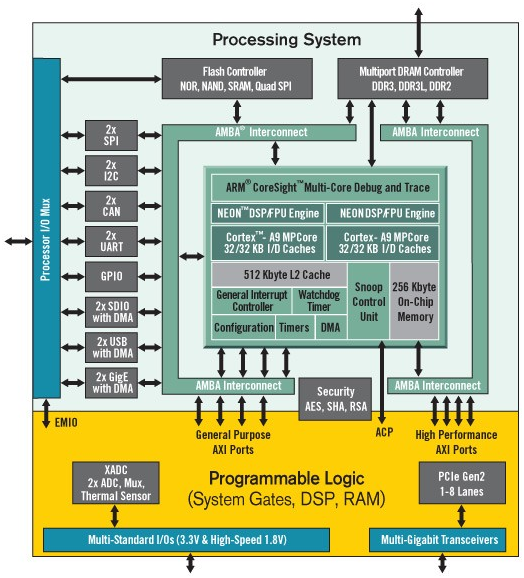
\includegraphics[width=12cm]{img/zyng-platform.png}
	\caption{Schemat architektury Zynq-7000. (Źródło: \cite{zybo-reference-manual})}
	\label{fig:zynq-overview}
\end{figure}
%TODO może nieco większy
% OK

Schemat przedstawia podział układu na części \emph{PL} -- oznaczonej kolorem żółtym, oraz \emph{PS} -- na zielono.
Architektura części programowalnej zbliżona jest do powszechnie stosowanych układów FPGA. %TODO konkretnie jaka seria Xilinx
% dodałem tę informację nieco wyżej
Wyposażono ją jednak w zbiór portów umożliwiających wydajną komunikację z procesorem. 
Ponadto, konfiguracja tej części wykonywana jest na starcie przez procesor lub przy użyciu interfejsu JTAG i układ nie zawiera elementów pozwalających na wykorzystanie logiki programowalnej niezależnie.
Część procesorowa wyposażona jest w szereg interfejsów, w tym kontroler pamięci DDR3, interfejs komunikacji AMBA oraz zbiór interfejsów peryferyjnych.

Procesor wyposażony jest w koprocesor arytmetyczny (\emph{FPU}), wspierający w obliczeniach na liczbach zmiennoprzecinkowych oraz wspiera obsługę architektury SIMD (\emph{ang.} Single Instruction, Multiple Data) -- pozwalającej na przetwarzanie wielu strumieni danych przy użyciu jednego strumienia instrukcji. 
Zagadnienia te szerzej opisane zostały w rozdziale \ref{sec:arm-neon}.
%TODO Tu dobrze by było się odwoływać do nazw bloków z rysunku (np. FPU).
% OK

Układ wyposażony jest w kontroler pamięci DDR, obsługujący żądania dostępu ze strony zarówno procesora, jak i logiki programowalnej. %TODO logiki programowalnej (bez powt. układ)
% OK
Pamięć jest współdzielona między obiema częściami. %TODO obiema częściami
% OK
Pozwala to na wymianę danych, do czego wykorzystywany jest standard AXI. Zastosowanie znajduje również mechanizm DMA, pozwalający na przeprowadzanie operacji z użyciem pamięci bez udziału procesora. 
Interfejs pozwala na transmisję pojedynczych słów danych, umożliwiając konfigurację parametrów pracy modułów algorytmicznych, jak i na transmisję o wysokiej przepustowości. 
Pozwala to, dzięki zastosowaniu modułu VDMA, na przesyłanie obrazu o rozdzielczości HD z częstotliwością osiągającą wartości 680 klatek na sekundę \cite{axi-vdma-guide}. 
Interfejs AXI opisano szerzej w rozdziale \ref{sec:axi-std}.

Dzięki zastosowaniu kontrolera przerwań (\emph{General Interrupt Controller}) możliwe jest wykorzystanie modułów logiki programowalnej komunikujących się z procesorem z wykorzystaniem techniki zgłaszania żądań. Zagadnienie to opisano w rozdziale \ref{sec:axi-interrupts}.

Ponadto, dostępne są powszechnie spotykane układy zegarowe (\emph{Timers}) i \emph{Watchdog}, odpowiedzialny za przerwanie pracy procesora w przypadku wykrycia błędnego wykonania programu.

Kontekst pamięciowy synchronizowany jest pomiędzy oboma rdzeniami procesora dzięki modułowi \emph{Snoop Control Unit}.

Układ logiki programowalnej należeć może do rodzin Artix-7 lub Kintex-7 i zbudowany jest z typowych elementów wykorzystywanych w FPGA o różnej liczebności, związanej z klasą układu:
\begin{itemize}
	\item CLB (\emph{ang.} Configurable Logic Blocks) -- w tym tablice Look-up (\emph{LUT}) -- $14400 - 277400$ elementów, przerzutniki (\emph{FF}) -- $28800 - 554800$ elementów.
	
	\item Pamięci \emph{Block RAM} -- od $1,8Mb$ do $26,5Mb$ ($50 - 755$ elementów).
	
	\item Elementy \emph{DSP} -- wykorzystywane zwykle do implementacji operacji dodawania i mnożenia -- $66 - 2020$ elementów.
	
	\item Bloki \emph{IOB} -- umożliwiające budowę interfejsów wejściowych i wyjściowych.
	
	\item Inne -- w tym interfejs JTAG, PCI Express czy konwertery analogowo-cyfrowe.
\end{itemize}
%TODO Brakuje choćby podstawowego opisu zasobów PL - dodać.
% OK dodałem opis
%TODO Proszę dodać opisy pozostałych elementów PS (choć 1-2 zdania na każdy bloczek)
% OK, dodałem te, które mogą być jakkolwiek istotne z mojej perspektywy.
%TODO Proszę napisać, dlaczego AXI i FPU opisane są później... 
% nie chciałem rozdzielać tych zagadnień na część teoretyczną i praktyczną. Wg mnie nie miałoby to sensu zwłaszcza dla FPU.

%TODO TO bym jakoś bardziej w kierunku rozdziału o systemach operacyjnych przekształcił (bo de facto o tym jest). Tylko wtedy Peta i inne to subsection (przeorganizować hierarchię)
% OK, poprawiłem
\section{Zastosowanie systemu operacyjnego}
\label{sec:arm-programming}

Centralny element architektury stanowi dwurdzeniowy procesor ARM. 
Jest on odpowiedzialny za przeprowadzenie konfiguracji logiki reprogramowalnej. 
Ponadto pozwala na wykonanie dowolnego programu użytkownika. 
Powszechnie stosowana jest konfiguracja \textit{bare-metal}, w której procesor wykonuje program zaprojektowany w pełni przez użytkownika. 
Pozwala to na uzyskanie możliwie największej kontroli nad pracą układu, ogranicza jednak możliwości wykorzystania pełni zasobów procesora oraz utrudnia projektowanie rozbudowanych aplikacji. Brak systemu operacyjnego ogranicza możliwość wykorzystania komunikacji sieciowej na etapie wykonania programu. Możliwości przechowywania wyników i logów aplikacji są niewielkie. Ponadto, użycie zewnętrznych bibliotek, w tym związanych z przetwarzaniem obrazów, takich jak OpenCV, jest niemożliwa. W efekcie, wykorzystanie konfiguracji pozbawionej systemu operacyjnego nie jest możliwe w przypadku aplikacji wymagających nadzoru bez fizycznego dostępu do układu czy przechowywania wyników.
%TODO może nieco więcej szczegółów i przede wszstykim, że brak OS.
% OK

W niniejszej pracy badano możliwość wykorzystania systemu operacyjnego Linux na przykładzie aplikacji systemów wizyjnych. 
Dzięki zastosowaniu Linuxa, możliwe staje się budowanie programów składających się z wielu modułów działających niezależnie. 
System ten wspiera obsługę sieci, co pozwala na wykorzystanie narzędzi komunikacji sieciowej, jak SSH \cite{ssh-protocol}, do konfiguracji i nadzorowania działania aplikacji, co opisano w rozdziale \ref{sec:ssh}. 
Ponadto, możliwe jest wykorzystanie powszechnie dostępnych bibliotek, ułatwiających rozwój aplikacji w krótkim czasie. 
Zagadnienie to badano na przykładzie biblioteki OpenCV \cite{opencv-library}, udostępniającej narzędzia przetwarzania obrazów, co opisano w rozdziale \ref{sec:opencv-lib}.

Zbadano możliwość wykorzystania systemu PetaLinux, rozwijanego przez organizację Xilinx, jak i podstawowej wersji systemu, opartej wyłącznie na źródle jądra, oraz dystrybucji bazującej na Ubuntu Core. %TODO co jest rozumiane przed podstawową wersję systemu ?
% OK?
Ponadto, rozpatrzono możliwość użycia systemu czasu rzeczywistego do wykonania zadań obliczeniowych z zachowaniem reżimu czasowego.
%TODO Wspomnieć o RTOS
% OK

\subsection{PetaLinux} %TODO Sub
% OK

Firma Xilinx zapewnia dostęp do zbioru narzędzi \emph{PetaLinux Tools} \cite{petalinux-tools} umożliwiających przeprowadzenie procesu konfiguracji, budowania i uruchamiania systemu Linux na platformie Zynq. 
Dzięki zintegrowaniu koniecznych narzędzi w jednym pakiecie, proces ten jest w dużej części zautomatyzowany i ogranicza interakcję z programistą, zapewniając przy tym możliwość dowolnej konfiguracji systemu.

Celem wykorzystania omawianego pakietu narzędzi jest zbudowanie systemu operacyjnego gotowego do uruchomienia i umożliwiającego szybką rekonfirugację zarówno elementów logiki reprogramowalnej jak i samego systemu operacyjnego.

Pakiet wymaga dostarczenia zewnętrznych zależności, w tym narzędzi umożliwiających budowanie systemu -- kompilatora, generatora parserów, systemu budowania -- oraz zbioru narzędzi programistycznych i konfiguracyjnych.
W przypadku dystrybucji Debian, zależności mogą być zainstalowane poleceniem:

\begin{lstlisting}[breaklines=true]
apt-get install tofrodos iproute2 gawk gcc git make net-tools libncurses5-dev tftpd zlib1g-dev libssl-dev flex bison libselinux1
\end{lstlisting}

W przypadku pracy na systemie wspierającym architekturę 64-bitową, konieczne jest również zainstalowanie bibliotek programistycznych dla architektury 32-bitowej.

\begin{lstlisting}[breaklines=true]
dpkg --add-architecture i386
apt-get update
apt-get install libc6:i386 libncurses5:i386 libstdc++6:i386
apt-get install libgtk2.0-0:i386 libxtst6:i386 gtk2-engines-murrine:i386 lib32stdc++6 libxt6:i386 libdbus-glib-1-2:i386 libasound2:i386
\end{lstlisting}

Praca z pakietem wymaga ponadto wykorzystania oprogramowania \emph{Vivado Design Suite} \cite{vivado-home} do zaprojektowania układu połączeń logiki reprogramowalnej oraz \emph{Xilinx SDK} \cite{xsdk-home} do kompilacji programów uruchamianych w środowisku systemu operacyjnego układu.

Pierwszym krokiem jest wykonanie projektu w pakiecie \emph{Vivado}. 
Szczegóły procesu opisano w rozdziale \ref{sec:vivado-conf}. %TODO sekcji -> rozdziale (wydaje mi się, ze w PL słowo sekcja nie powinno być uzywane w tym kontekście - kalka z ENG)
% OK, poprawię masowo w całej pracy na końcu 1. korekty
Wyeksportowany projekt Vivado jest konieczny do przeprowadzenia procesu budowania systemu, proces konfiguracji projektu PetaLinux opisano w rozdziale \ref{sec:petalinux-config}. %TODO akapity jednozdaniowe są zakazane...
% OK, spróbuję je wyłapać

Pakiet udostępnia możliwość dodania do budowanego systemu zbioru programów i bibliotek. 
Dostępne jest kilkaset pakietów oprogramowania oferowanych na zasadach wolnych licencji, w tym biblioteki do przetwarzania obrazów. %TODO Dostępne, dostępnego
% OK
Ponadto, pakiet umożliwia dodanie własnoręcznie zbudowanych aplikacji. 
Pozwala to na integrację etapu projektowania aplikacji oraz budowy i uruchamiania systemu operacyjnego w jednym procesie.

Projekt PetaLinux jest niezależny od projektu Vivado i może powstawać równolegle. 
Zmiany w strukturze modułów logiki reprogramowalnej wymagają ponownego zbudowania plików wynikowych systemu operacyjnego PetaLinux, jednak proces ten został wydzielony z oprogramowania Vivado. %TODO co tu jest rozumiane przez system
% OK
Pozwala to na wykorzystanie jednego projektu opisującego logikę współpracującego z aplikacjami bare metal i systemowymi. 

Proces budowania systemu jest czasochłonny, na etapie prototypowania aplikacji praktyczne jest zastosowanie oprogramowania pracującego w trybie bare-metal. %TODO bare-metal - pisałbym w \textit{} 
% OK, poprawię masowo na koniec
Pozwala to na przeprowadzanie procesu debugowania aplikacji bezpośrednio z poziomu oprogramowania Vivado/SDK. 
Po upewnieniu się, że sprzętowa część algorytmu działa poprawnie, zaprojektować można aplikację systemową, odpowiedzialną za komunikację, monitorowanie i wykorzystanie wyników działania algorytmu w kompletnym projekcie.

\subsection{Inne dystrybucje systemu}
Niezależnie do analizy zastosowania PetaLinux, zbadano również inne możliwości konfiguracji systemu operacyjnego do zastosowania na platformie ZYBO. 
Wśród dostępnych opcji, rozpatrzono dystrybucję Ubuntu Core oraz budowę systemu Linux ze źródeł.
%TODO ponieważ to jest część teoretyczna, to proszę nie wprowadzać takie narracji po zapozaniu...
% OK?

\subsubsection{Budowa ze źródeł}
Wykorzystanie pakietu PetaLinux związane jest z ograniczeniem dostępności projektu do środowisk, dla których ten pakiet narzędzi jest dostępny. 
W przypadku konieczności uruchomienia projektu na systemie nie wspieranym przez twórców oprogramowania lub potrzeby wprowadzenia dużych zmian w kodzie źródłowym systemu i konfiguracji, konieczne może być przeprowadzenie pełnego procesu budowania samodzielnie. 
Takie podejście pozwala również na pełne zrozumienie znaczenia kolejnych kroków procesu konfiguracji.

Proces budowy systemu składa się z kilku kroków. 
\begin{enumerate}
\item Plik binarny zawierający konfigurację części oprogramowania wykorzystującej logikę programowalną dołączany jest w trakcie procesu budowania systemu operacyjnego.%TODO co tu jest rozumiane przez zaprojektowanie połączeń logiki reprogramowalnej
% OK, zmieniłem to zdanie

\item Konieczne jest zbudowanie dwóch programów rozruchowych (\emph{ang.} bootloader). %TODO program rozruchowy to poprawne określenie PL ?
% wikipedia mówi, że tak, dodałem angielskie znaczenie
Pierwszy z nich -- FSBL (\emph{ang.} First Stage Boot Loader) -- odpowiada za przeprowadzenie procesu wstępnej konfiguracji procesora, kontrolera pamięci i uruchomienie drugiego programu rozruchowego. 
Na drugim etapie rozruchu wykorzystywany jest program U-Boot. 
Jego zadaniem jest przygotowanie środowiska do uruchomienia właściwego systemu operacyjnego.

\item Kolejny krok wymaga zbudowania struktury drzewa urządzeń (\emph{ang.} device tree). 
Pozwala ona na zdefiniowanie i konfigurację urządzeń połączonych z procesorem, dzięki czemu mogą być one obsłużone przez system operacyjny. 
W przypadku układu Zynq, wykorzystanie tej struktury pozwala na konfigurację i komunikację z elementami układu FPGA. %TODO ZYBO czy Zynq...
% Poprawiłem

\item Po przeprowadzeniu wstępnej konfiguracji elementów systemu, możliwe jest wykonanie procesu konfiguracji, budowania i przygotowania wynikowych plików binarnych.
\end{enumerate}
Opisany proces jest skomplikowany i wymaga specjalistycznej wiedzy. 
Dostępne są obszerne opracowania dotyczące tematu, zawierające precyzyjny opis kolejnych wymaganych kroków \cite{zybo-zynq-getting-started,zybo-stock-linux,xilinx-build-kernel}.

%TODO A Pan to robił ? Jeśli tak to link to szczegółowego opisu.
% robiłem, ale na bazie źródeł, które cytuję powyżej. Proces jest dość skomplikowany i podatny na zmiany, ze względu na liczbę narzędzi, które się wykorzystuje, więc nie widziałem sensu budowania kolejnego tutoriala.

\subsubsection{Ubuntu Core}

Ubuntu Core to dystrybucja systemu Linux dedykowana do zastosowań w urządzeniach tzw. internetu rzeczy (IoT -- \emph{ang.} Internet of Things). %TODO (IoT ang.....) nie wiem czy nie lepiej koncepcji -> tzw.
% OK?
Dystrybucja ta oparta jest na podstawowej wersji systemu Ubuntu, przystosowana do uruchomienia na urządzeniach o ograniczonej mocy obliczeniowej.

Dzięki wykorzystaniu Ubuntu Core, możliwy jest dostęp do repozytorium oprogramowania udostępnianego przez dystrybucję. 
W przeciwieństwie do dystrybucji PetaLinux, instalowane oprogramowanie może być aktualizowane w trakcie pracy systemu. 
Cecha ta może być istotna w przypadku aplikacji działających przez długi czas, gdy aktualizacja oprogramowania jest korzystna ze względu na znalezione błędy lub poprawę bezpieczeństwa w kolejnej wersji. %TODO bezpieczeństwo.
% ok?

System Ubuntu Core może być zbudowany i uruchomiony na karcie ZYBO przy użyciu dedykowanego narzędzia \cite{ubuntu-core-zybo}.
%TODO Uwaga tak jak wcześniej...
% OK

\subsection{RTOS}

System operacyjny czasu rzeczywistego (\emph{RTOS}, \emph{ang.} Real Time Operating System) to system operacyjny, którego zadaniem jest obsługa aplikacji przy zachowaniu założeń o nieprzekroczeniu maksymalnego dopuszczalnego czasu odpowiedzi programu. 
Pozwala to na projektowanie aplikacji, w których czas odpowiedzi ma kluczowe znaczenie, w tym systemów sterowania lub krytycznych aplikacji wizyjnych.
Dzięki zastosowaniu dwurdzeniowego procesora w układzie Zynq, rozważyć można zaprojektowanie rozwiązania, w których jeden z rdzeni odpowiada za wykonanie programu Linuxa, a drugi -- aplikacji lub systemu czasu rzeczywistego. %TODO ZYBO/Zynq - aplikacji \textit{bare metal}
% OK

Rozpatrzono możliwość uruchomienia systemu operacyjnego PetaLinux i jego współpracę z aplikacjami czasu rzeczywistego na przykładzie OpenAMP \cite{openamp-home}. 
OpenAMP zapewnia interfejs umożliwiający komunikację pomiędzy programami działającymi w systemie Linux oraz aplikacjami czasu rzeczywistego, wykorzystując do tego narzędzia dostępne już w systemie.
Z punktu widzenia klasycznego systemu operacyjnego, program działający na systemie czasu rzeczywistego jest zewnętrznym zasobem, który oczekuje na zlecenie wykonania konkretnego zadania i wysyła odpowiedź.
Dzięki wykorzystaniu systemu czasu rzeczywistego FreeRTOS \cite{freeRTOS-home}, aplikacje mogą mieć dostęp do zasobów systemowych, w tym pamięci i interfejsów komunikacji.

%TODO Za krótkie akapity - proszę zobaczyć jak to wygląda w txt
% Poprawiłem

System czasu rzeczywistego może być wykorzystany do obliczeń o krytycznym znaczeniu. 
W przypadku wykorzystania klasycznego systemu operacyjnego, nie jest możliwe zagwarantowanie wykonania dowolnego zadania w określonym czasie. 
W trakcie działania aplikacji, system może zadecydować o jej czasowym zatrzymaniu i udostępnieniu zasobów innemu z oczekujących zadań. 
Aplikacja działająca w czasie rzeczywistym pozwala uniknąć tego zjawiska.

System PetaLinux oferuje dostęp do modułów \texttt{RPMsg}, \texttt{remoteproc}, \texttt{virtIO}, które są wymagane do zapewnienia komunikacji z systemem czasu rzeczywistego. 
Udostępnione zostały również aplikacje testowe, które pozwalają na sprawdzenie poprawności działania konfiguracji.
Użycie systemu czasu rzeczywistego wymaga zmian projektowych, w tym konfiguracji dwóch instancji konsoli do komunikacji szeregowej i zdefiniowania struktury drzewa urządzeń określającej obszar pamięci dla obu systemów operacyjnych. 
Po zbudowaniu poprawnie skonfigurowanego systemu i jego uruchomieniu, przetestowanie działania aplikacji wymaga użycia poniższych poleceń.

\begin{lstlisting}[breaklines=true]
modprobe zynq_remoteproc firmware=image_echo_test
modprobe rpmsg_user_dev_driver
echo_test
\end{lstlisting}

W rezultacie uruchomiono moduły odpowiedzialne za obsługę systemu czasu rzeczywistego i przeprowadzono test komunikacji. %TODO W rezultacie uruchomione...
% OK
Konfiguracja i wykorzystanie systemów czasu rzeczywistego wykracza poza zakres niniejszej pracy, a zagadnienie jest obiektem obszernych opracowań \cite{adam-taylor-openamp,zynq-openamp-gsg}.

%TODO to źle kojarzę, że coś Pan z tym eksperymentował ?
% sprawdzałem to, ale moje wnioski właściwie przeczyły temu, co znalazłem w innych źródłach. Tzn. ja to w jakimś stopniu "zhackowałem", Xilinx upiera się, że wymagane jest dostarczenie BSP dedykowanej dwóm systemom, moje próby zbudowania BSP spełzły na niczym, ale gdy uruchomiłem `echo_test` na domyślnej konfiguracji, to jeden rdzeń procesora "zniknął" z Peta i zaczął działać real-time. Ten temat był dopiero rozwijany przez Xilinx gdy nad tym pracowałem, spodziewałbym się, że uporządkują to w przyszłości, bo mocno forsują swoje rozwiązanie - więc nie chciałem opisywać tutaj żadnych niepełnych rozwiązań...

\subsection*{Podsumowanie} %TODO dlaczego to nie ma tytułu. Może to przenieć na koniec jako podsumowanie OS, tylko dodać coś o RTOS.
% OK

Zarówno wykorzystanie pakietu PetaLinux Tools, jak i obu pozostałych metod pozwala na zbudowanie w pełni funkcjonalnej dystrybucji systemu Linux i uruchomienie jej na układzie Zynq. %TODO karcie/Zynq
%OK
Każda z metod wiąże się z innymi ograniczeniami i udostępnia inne możliwości. 
W przypadku użycia narzędzi PetaLinux, użytkownik uzyskuje dostęp do ograniczonego zbioru dodatkowych aplikacji, niewielkiej w porównaniu do repozytoriów udostępnianych w dystrybucji Ubuntu Core. 
Ponadto aktualizacja oprogramowania może wymagać ponownego zbudowania systemu lub nie być możliwa bez aktualizacji pakietu narzędzi. 

Dystrybucja Ubuntu Core zapewnia dostęp do aktualizacji samego systemu, pozwalając na zachowanie bezpieczeństwa działania i dostęp do poprawek kodu oprogramowania. 
Może to być kluczowe w przypadku wykorzystania układu Zynq do działania przez długi czas z oczekiwaną niezawodnością. %TODO ZYBO/Zynq
% OK

W przypadku konieczności dostosowania kodu systemu operacyjnego do własnych potrzeb, praktyczne staje się natomiast wykorzystanie technik budowy systemu bezpośrednio ze źródeł. 
Ogranicza to jednak możliwości instalacji dodatkowego oprogramowania i wymaga dobrej znajomości zagadnień związanych z działaniem systemu Linux.

Pakiet PetaLinux pozwala jednak na największą integrację z oprogramowaniem Vivado, co ułatwia prototypowanie aplikacji. 
Dzięki udostępnieniu repozytorium oprogramowania oraz braku konieczności ingerencji użytkownika w proces budowania systemu, wykorzystanie go jest najlepszym rozwiązaniem w większości projektów. 
Z tego powodu, w niniejszej pracy zdecydowano się na użycie tego rozwiązania na dalszym etapie projektu.

Zastosowanie systemu czasu rzeczywistego współpracującego z innym systemem operacyjnym pozwala na wykonanie krytycznych sekcji kodu z zachowaniem ograniczeń czasowych. Pamiętać należy jednak, że wiąże się to z ograniczeniem maksymalnej wydajności operacji wykonywanych przez klasyczny system operacyjny.

Firma Xilinx zrezygnowała ze wsparcia dla systemu FreeRTOS i podobnych i zdecydowano się na oparcie na bibliotece OpenAMP do realizacji zadań wykonywanych w czasie rzeczywistym. W okresie powstawania pracy, literatura omawiająca integrację biblioteki z systemem operacyjnym dla kart innych producentów nie była powszechnie dostępna. Z tego powodu, realizacja omawianych zadań w przypadku karty ZYBO była poważnie utrudniona.

\chapter{Przegląd wybranych funkcjonalności platformy Zynq i systemu operacyjnego PetaLinux}
\label{cha:functionalities}

W ramach pracy przeprowadzono analizę wybranych funkcjonalności układów rodziny Zynq działających pod kontrolą systemu operacyjnego PetaLinux, które mogą zostać zastosowane podczas realizacji wbudowanych systemów przetwarzania obrazów. 
Wybrane zagadnienia przedstawiono w poniższych podrozdziałach.

\section{Obsługa SSH}
\label{sec:ssh}

Po połączeniu karty z uruchomionym systemem PetaLinux z komputerem przez interfejs USB, możliwe jest otworzenie konsoli komunikacji przy użyciu protokołu transmisji szeregowej.
Komunikacja odbywa się z prędkością 115200 bodów, ośmioma bitami danych, jednym bitem stopu i bez bitu parzystości. %TODO tu akurat do karty, ponadto chyba trzeba jeszcze coś zaprogramować... czy uruchomić.
% OK

Komunikacja przy użyciu transmisji szeregowej jest jednak ograniczona do sytuacji, w których możliwy jest bezpośredni dostęp do układu. 
Ponadto, nie zapewnia wysokiej przepustowości transmisji czy możliwości przesyłu plików. 
Z tych powodów, korzystne staje się wykorzystanie protokołu SSH (\emph{ang.} Secure Shell) do nawiązania komunikacji sieciowej. %TODO Rozwinięcie SSH + ew. 2-3 zadnie o samym protokowel (choćby na podstawie https://pl.wikipedia.org/wiki/Secure_Shell})
SSH jest najczęściej stosowanym protokołem bezpiecznej komunikacji, wspieranym przez zdecydowaną większość dystrybucji systemu Linux i nie wymagającym dodatkowej konfiguracji na etapie budowania systemu. Dzięki zastosowaniu technik szyfrowania połączenia, zapewnia mechanizm nawiązywania kryptograficznie bezpiecznej komunikacji między dwoma urządzeniami. Wśród najczęściej wykorzystywanych funkcji protokołu wymienić można udostępnienie zdalnej konsoli poleceń, przesyłanie plików czy tunelowanie połączeń.

Połączenie odbywa się przy użyciu poniższego polecenia.

\begin{lstlisting}[breaklines=true]
ssh root@(*@\textit{adres-ip-urządzenia}@*) 
\end{lstlisting} %TODO ta końćówka jest poprawna ?
% poprawiłem

Domyślne hasło administratora w przypadku dystrybucji PetaLinux to \texttt{root}. 
Może być ono zmienione na etapie konfiguracji systemu z wykorzystaniem poniższych poleceń. %TODO z wykorzystaniem poniżzych poleceń:
% OK

\begin{lstlisting}[breaklines=true]
petalinux-config -c rootfs
Petalinux RootFS Settings -> Root password
\end{lstlisting}

Aby uprościć proces logowania, wykorzystać można mechanizm wymiany kluczy, zapewniany przez protokół. Weryfikacja obu stron połączenia przy użyciu kluczy wykorzystuje techniki kryptografii asymetrycznej. Użytkownik posiada parę związanych ze sobą kluczy kryptograficznych, umownie nazywanych kluczem publicznym i prywatnym. Wiadomość zaszyfrowana przy użyciu klucza publicznego może zostać odszyfrowana wyłącznie z użyciem klucza prywatnego. Użytkownik udowodnić może swoją tożsamość przez przesłanie oryginału otrzymanej wiadomości, zaszyfrowanej przy użyciu klucza publicznego.
Korzystając z tej zależności, klucz publiczny może być powszechnie znany i wykorzystywany do budowania kryptograficznie bezpiecznych wiadomości, pod warunkiem zachowania klucza prywatnego w tajemnicy.

Algorytmy kryptografii asymetrycznej wykorzystywane są przez narzędzie SSH na etapie weryfikacji tożsamości obu stron komunikacji. Po nawiązaniu połączenia, komunikacja zabezpieczana jest wybranych algorytmem symetrycznym. Wykorzystanie mechanizmu kluczy wymaga użycia poniższego polecenia.
%TODO nieco więcej o tym mechanizmie ?
% OK

\begin{lstlisting}[breaklines=true]
ssh-copy-id -i ~/.ssh/id_rsa.pub root@(*@\textit{adres-ip-urządzenia}@*)
\end{lstlisting}

Umożliwia to logowanie w przyszłości bez konieczności podania hasła użytkownika. 
Skonfigurowany w opisany sposób protokół daje dostęp do pełnego zbioru narzędzi, w tym zdalnej obsługi konsoli użytkownika, przesyłania plików, tunelowania portów czy zdalnego montowania systemów plików.

\section{FPU i technologia NEON}

\label{sec:arm-neon}

Układ Zynq wyposażony jest w koprocesor arytmetyczny oraz wspiera polecenia wykorzystujące technologię NEON \cite{neon-home}. %TODO ZYBO -> Zynq
% OK
Elementy te pozwalają na zwiększenie wydajności projektowanych aplikacji w przypadku, gdy wykonywane operacje wymagają przeprowadzania obliczeń na liczbach zmiennoprzecinkowych lub działań wektorowych. 

Koprocesor arytmetyczny, FPU (\emph{ang.} Floating-point unit), to układ działający we współpracy z jednostką procesora, dedykowany do wykonywania obliczeń na liczbach zmiennoprzecinkowych. 
Wykorzystanie dedykowanego układu pozwala na zwiększenie szybkości wykonywania operacji arytmetycznych, pierwiastkowania i przesunięć bitowych. 
W przypadku braku dedykowanego układu FPU, konieczne jest symulowanie jego działania dla jednej operacji na liczbach zmiennoprzecinkowych przez wykonywanie większej liczby operacji na typach całkowitych, co wiąże się ze spadkiem wydajności. %TODO całkowitych czy stałoprzecinkowych...
% jedna operacja float dzielona jest na wiele operacji int, wyznaczanie cechy, mantysy, etc. Sprecyzowałem.

Technologia NEON pozwala na rozszerzenie puli rozkazów procesora ARM o polecenia wykorzystujące architekturę SIMD zdefiniowaną przez taksonomię Flynna \cite{Flynn1972}.
SIMD (\emph{ang.} Single Instruction stream, Multiple Data streams) to klasa systemów, które pozwalają na przetwarzanie wielu strumieni danych na podstawie jednego strumienia instrukcji. 
Zastosowania tej architektury obejmują zagadnienia, w których dla wielu wartości wejściowych konieczne jest wykonanie tej samej operacji. 
Cechę tę posiada wiele operacji związanych z przetwarzaniem sygnałów i obrazów, w tym  wyznaczanie wartości szybkiej transformaty Fouriera, implementacje filtrów FIR i IIR czy operacje skalowania, rotacji i filtracji uśredniającej obrazu.

Rozpatrzono możliwość wykorzystania architektury NEON w zagadnieniach przetwarzania sygnałów. 
Działanie testowano na podstawie programu wyznaczającego wartość iloczynu skalarnego dwóch wektorów zadanej długości. 
Porównano trzy implementacje algorytmu, którego kod źródłowy zawarto w dodatku \ref{cha:neon-source}.
Wykorzystano implementację bazową oraz stosującą polecenia dostępne w architekturze NEON i porównano wyniki z implementacją zaprojektowaną w asemblerze. %TODO powt. wykorzystano
% OK

Implementacja w architekturze NEON wykorzystuje dedykowane funkcje, udostępnione w bibliotece \texttt{arm\_neon.h}, które mają na celu maksymalne zwiększenie wydajności aplikacji. 
W przypadku pozostałych implementacji, stosowane są polecenia wykonywane na koprocesorze VFP (\emph{ang.} Vector Floating-Point). 
VFP to układ niezależny od FPU, pozwalający na wykonanie jednej instrukcji dla wektora danych wejściowych. 
Układ ten nie należy do rodziny SIMD i wykonuje instrukcje sekwencyjnie, w przeciwieństwie do architektury NEON.
%TODO Za dużo razy "wykorzystuje". Druga spraw to VFP - to jest element FPU ?
% OK, sprecyzowałem


\begin{table}[h]
	\caption{Wyniki testu wydajnościowego.}
	\centering
	\label{tab:neon-time-results}
	\begin{tabular}{|l|l|l|l|}
		\hline
		\multicolumn{4}{|c|}{Bez optymalizacji} \\ \hline
		Implementacja & min {[}s{]} & max {[}s{]} & średnio {[}s{]} \\ \hline
		Bazowa & 0,4266 & 0,4339 & 0,4296 \\ \hline
		NEON & 0,1103 & 0,1108 & 0,1105 \\ \hline
		ASM & 0,4082 & 0,4086 & 0,4083 \\ \hline
		\multicolumn{4}{|c|}{Z optymalizacjami} \\ \hline
		Bazowa & 0,1080 & 0,1152 & 0,1092 \\ \hline
		NEON & 0,1088 & 0,1147 & 0,1090 \\ \hline
		ASM & 0,1087 & 0,1144 & 0,1089 \\ \hline
	\end{tabular}
\end{table}

Eksperyment przeprowadzono z wykorzystaniem karty ZYBO działającej pod kontrolą systemu PetaLinux.
%TODO A ten ekxperyment to pod linuzem był ? Jak tak to napisać...
% OK
Rozpatrzono przeprowadzenie procesu komplikacji z wyłączonymi optymalizacjami kompilatora (flaga \texttt{-O0}) oraz z włączonymi wszystkimi optymalizacjami (\texttt{-O3}).
Wykorzystane poleceń NEON wymaga użycia odpowiadających im parametrów kompilacji. 
Poniżej przedstawiono polecenie kompilacji testowej implementacji wykorzystującej NEON.

\begin{lstlisting}[breaklines]
arm-linux-gnueabihf-gcc -Wall -O3 -mcpu=cortex-a9 -mfpu=neon -ftree-vectorize -mvectorize-with-neon-quad -mfloat-abi=hard -ffast-math -funsafe-math-optimizations -g -c -o "src/main.o" "../src/main.c"
\end{lstlisting}

Wyniki testów wydajności zebrano w tabeli \ref{tab:neon-time-results}. %TODO to zdanie przenieść później bezpośrednio przed analizę wyników.
% OK
W sytuacji, gdy wyłączono optymalizację na etapie kompilacji, zauważalny jest znaczny wzrok wydajności w przypadku wykorzystania instrukcji udostępnianych przez architekturę NEON. 
Pozwala ona na niemal czterokrotne zwiększenie szybkości działania programu względem pozostałych implementacji. 
Różnica ta zanika w przypadku wykorzystania możliwości optymalizacji kodu programu na etapie kompilacji. 
Różnica w szybkości wykonania programu NEON jest niewielka, gdyż pozostałe implementacje zostały zoptymalizowane do stanu, w którym koszt ich wykonania porównywalny jest z implementacją w NEON. %TODO jednak -> gdyż ?
% OK

Wyniki pozwalają wnioskować o słuszności wykorzystania instrukcji udostępnianych przez architekturę NEON ze względu na możliwy wzrost wydajności. Istotna jest jednak weryfikacja wyników i potwierdzenie poprawy działania aplikacji. 
W przypadku, gdy różnice między programami są niewielkie, użycie instrukcji NEON może być niekorzystne ze względu na zwiększoną latencję wykonania rozkazów.

%TODO No dobrze, a wie Pan dlaczego tak się stało ??? Czy zły przykład, czy optymalizacja wykorzytstuje tego NEONA, czy jak ? Ew. proszę to jeszcze jakoś sprawdzić...
% Przykład powinien być dobry, bo mierzę czas wykonania samej sekcji krytycznej, a sam eksperyment zajmuje kilka minut, więc zakłócenia powinny być niewielkie. Postarałem się też "utrudnić" optymalizacje kompilatorowi, losując dane wejściowe przed każdą iteracją, etc. Jedyne co mi przychodzi do głowy, to że procesor mógł rozsądnie pipeline'ować instrukcje, bo nie robił żadnych dziwnych skoków, etc.
% Konfiguracja też wyglądała dobrze, spróbowałem jeszcze raz przetestować, z dodatkową flagą kompilacji, która mogła pomóc, ale nie zauważyłem różnicy. I dwie z implementacji używają instrukcji VFP, sądzę, że dlatego wydajność jest porównywalna.

\section{Protokół AXI}
\label{sec:axi-std}

Protokół AXI (\emph{ang.} Advanced eXtensible Interface) zdefiniowany został w specyfikacji AMBA (\emph{ang.} Advanced Microcontroller Bus Architecture) 3. 
W kolejnej wersji dokumentu sprecyzowano standard w najnowszej wersji -- AXI4 \cite{axi-spec}. 
Protokół wykorzystywany jest do komunikacji pomiędzy elementami układu lub modułami zbudowanymi wewnątrz logiki reprogramowalnej i jest dedykowany systemom o dużej wydajności i pracującym z wysoką częstotliwością.

Specyfikacja definiuje trzy typy interfejsu:
\begin{itemize}
	\item AXI4 -- wykorzystujące technikę MMIO (\emph{ang.} Memory-Mapped Input/Output) do odwzorowania rejestrów w przestrzeni adresowej pamięci RAM i dedykowanej aplikacjom wymagającym dużej wydajności komunikacji.
	\item AXI4-Lite -- uproszczona wersja protokołu, wykorzystująca MMIO i dedykowana aplikacjom o mniej rozbudowanych wymaganiach komunikacyjnych.
	\item AXI4-Stream -- wersja przepływowa protokołu, nie wykorzystująca technik MMIO.
\end{itemize}

Interfejsy wykorzystujące technikę MMIO stosowane są powszechnie w zadaniach konfiguracji modułów aplikacji czy przesyłania informacji, takich jak ramka sygnału wizyjnego do pamięci procesora. 
Dzięki reprezentacji stanu elementów logiki reprogramowalnej w postaci komórek pamięci operacyjnej procesora, możliwa jest jednolita analiza działania całego systemu. %TODO w jakim sensie "w pamięci".
% OK?

Interfejs w wersji \emph{Stream} wykorzystywany jest natomiast do przesyłania sygnału pomiędzy kolejnymi elementami układu, na przykład transmisji kolejnych pikseli obrazu pomiędzy kolejnymi składowymi algorytmu przetwarzania obrazu. 
Proces przesyłania danych w takiej formie charakteryzuje się większą wydajnością, analiza działania aplikacji jest jednak utrudniona ze względu na brak reprezentacji przesyłanych danych w pamięci.

Możliwe jest również połączenie obu typów interfejsu wewnątrz jednego elementu. 
Technika ta wykorzystana została w przypadku elementu AXI VDMA, umożliwiając manipulowanie ramkami obrazu wizyjnego przesyłanymi przy użyciu interfejsu \emph{Stream} dzięki buforowaniu w pamięci RAM. 
Zagadnienie to szerzej opisano w rozdziale \ref{sec:axi-vdma}. 
Podobne techniki wykorzystano również w przypadku interfejsu Ethernet DMA, umożliwiającego komunikację przy użyciu protokołu Ethernet.

\subsection{Przebieg transakcji}

Transakcja komunikacyjna odbywa się pomiędzy dwoma urządzeniami -- \emph{master} i \emph{slave}, jednak dzięki zastosowaniu elementów AXI-Interconnect możliwe jest połączenie wielu urządzeń, co przedstawiono na schemacie \ref{fig:axi-interconnect}.

\begin{figure}[h]
	\centering
	\def\svgwidth{8cm}
	\input{img/axi-interconnect.pdf_tex}
	\caption{Schemat połączenia Interconnect w protokole AXI.}
	\label{fig:axi-interconnect}
\end{figure}


Komunikacja odbywa się przy użyciu pięciu niezależnych kanałów:
\begin{itemize}
	\item Read Address
	\item Write Address
	\item Read Data
	\item Write Data
	\item Write Response
\end{itemize}

Każdy kanał zawiera zbiór sygnałów wykorzystywanych w trakcie wymiany danych.

Transmisja rozpoczyna się od wykorzystania sygnałów \emph{valid} i \emph{ready}. 
Urządzenie źródłowe wymusza stan wysoki sygnału \emph{valid} i oczekuje na zmianę wartości sygnału \emph{ready} urządzenia docelowego na stan wysoki. 
W chwili, gdy oba sygnały znajdują się w tym stanie, właściwe dane mogą zostać przesłane z urządzenia źródłowego do docelowego. 
Pozwala to na przekazanie takich danych jak adres odczytu/zapisu do pamięci, odczytywanych lub zapisywanych danych i potwierdzenia zapisu. 
Proces nawiązania transakcji odbywa się niezależnie dla każdego wykorzystywanego kanału.

Procedura odczytu danych składa się z dwóch etapów:
\begin{enumerate}
	\item Zdefiniowanie  przez urządzenie \emph{master} adresu i parametrów transmisji danych na kanale \emph{Read Address}.
	\item Przesłanie przez urządzenie \emph{slave} jednej lub więcej wartości danych na kanale \emph{Read Data}.
\end{enumerate}

Natomiast procedura zapisu wymaga trzech etapów:
\begin{enumerate}
	\item Zdefiniowanie  przez urządzenie \emph{master} adresu i parametrów transmisji danych na kanale \emph{Write Address}.
	\item Przesłanie przez urządzenie \emph{master} jednej lub więcej wartości danych na kanale \emph{Write Data}.
	\item Przesłanie przez urządzenie \emph{slave} odpowiedzi na kanale \emph{Write Response}.
\end{enumerate}

Protokół pozwala ponadto na przesłanie do 256 wartości danych w trakcie jednej transmisji dzięki technice \emph{burst}, a transakcje odczytu i zapisu danych mogą odbywać się równolegle.

Przepływ danych w interfejsie AXI4-Stream odbywa się wyłącznie w jednym kierunku i nie jest możliwy odczyt danych przesłanych wcześniej przez urządzenie \emph{master} do \emph{slave}. 
Procedura ta jest podobna do transakcji zapisu, jest jednak rozszerzona o możliwość dzielenia operacji na kilka mniejszych i łączenia wielu transakcji w jedną.

\subsection{AXI DMA}

DMA (\emph{ang.} Direct Memory Access) to technika często stosowana w przypadku konieczności wykonywania operacji na pamięci RAM urządzenia z dużą szybkością. %TODO a nie wydajnością, szybkością
% OK
Wykorzystanie kontrolera DMA pozwala przeprowadzać operacje odczytu i zapisu do pamięci operacyjnej bez konieczności użycia głównej jednostki procesora. 
Dzięki temu, procesor odpowiada wyłącznie za skonfigurowanie kontrolera DMA i może wykonywać inne operacje w trakcie transmisji danych. 
Ponadto, stosowanie kontrolera DMA pozwala zwykle na uzyskanie wyższej przepustowości komunikacji z pamięcią i zmniejszenie zużycia energii.
Kontroler DMA może również przeprowadzać podstawowe operacje konwersji sygnałów, na przykład, w przypadku sygnału wizyjnego, konwersję sygnałów synchronizacji obrazu -- kontroler odpowiada za odpowiednie wyrównanie (\emph{ang.} alignment) danych w pamięci, tak by zachować odstępy poprawnej długości pomiędzy kolejnymi liniami obrazu. %TODO nie za bardzo rozumiem... 
% OK?

DMA pozwala na przesłanie wielu wartości danych w ramach jednej transakcji w trybie \emph{burst}. 
\emph{Master} przesyła wyłącznie adres pierwszego bajta danych, a kolejne adresy wyznaczane są w trakcie operacji przez urządzenie \emph{slave}.
Wyznaczany adres może być zwiększany, w przypadku, gdy operacja wykonywana jest w pamięci, bądź mieć stałą wartość, co ma miejsce w przypadku zapisu lub odczytu z kolejki FIFO (\emph{ang.} First In, First Out). 
Interfejs pozwala również na ograniczenie dostępnej przestrzeni adresowej, w efekcie czego wartość adresu po przekroczeniu górnej granicy zakresu przyjmuje ponownie najniższą dopuszczalną wartość. 
Własność ta może być wykorzystana do projektowania linii buforujących.

Protokoły transmisji danych wykorzystywać mogą kolejność bajtów od najmniej znaczącego lub odwrotną. Należy o tym pamiętać na etapie projektowania modułów odpowiedzialnych za proces komunikacji. Protokół AXI DMA wykorzystuje kolejność bitów, w której najmniej znaczący bajt umieszczony jest jako pierwszy. %TODO akakpit-zdanie !
% OK

Dzięki zastosowaniu techniki DMA możliwa jest konfiguracja parametrów pracy algorytmu zaprojektowanego w układzie logiki reprogramowalnej oraz obserwacja jego działania na etapie wykonania z poziomu procesora ARM. Moduł algorytmiczny może udostępniać rejestry konfiguracyjne w przestrzeni adresowej pamięci procesora, a wyniki działania programu mogą być przesyłane do pamięci operacyjnej.%TODO niejasne dla mnie...
% poprawiłem
W szerszej perspektywie, pozwala to na udostępnienie interfejsu użytkownika, umożliwiającego nadzór nad pracą algorytmu, na przykład z poziomu konsoli dostępnej przez \emph{ssh} lub w formie interfejsu strony internetowej. 
Możliwe jest również przesyłanie powiadomień z elementów logiki programowalnej do procesora ARM w celu wymuszenia reakcji na osiągnięty stan programu, na przykład przesłanie informacji o ukończeniu iteracji algorytmu dla aktualnej ramki obrazu. %TODO możliwe-umożliwiające.
% OK
Można w tym celu wykorzystać mechanizm przerwań systemowych, co szerzej opisano w sekcji \ref{sec:axi-interrupts}.
%TODO nie za bardzo rozumiem ten akapit.... może Pan jakoś jaśniej opisać ?
% OK?

Mechanizm DMA zbadano na przykładzie projektu modułu umożliwiającego modyfikację parametrów oraz odczyt aktualnego stanu parametrów. 
Schemat strukturalny modułu przedstawiono na rysunku \ref{fig:axi-dma-diagram}.

\begin{figure}[h]
	\centering
	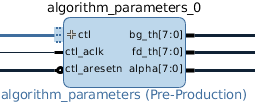
\includegraphics[]{img/algorithm-parameters.png}
	\caption{Graficzna reprezentacja modułu AXI DMA w programie Vivado.}
	\label{fig:axi-dma-diagram}
\end{figure}

Moduł wyposażony jest w interfejs AXI, podpisany \texttt{ctl} oraz związane z nim sygnały, zegarowy -- \texttt{ctl\_aclk} oraz reset -- \texttt{ctl\_aresetn}. 
Sygnały wyjściowe pozwalają na odczyt zdefiniowanych parametrów z poziomu innych modułów logiki reprogramowalnej. 
Dzięki wydzieleniu modułu odpowiedzialnego za konfigurację algorytmu z części wykonującej obliczenia algorytmiczne, możliwe jest uproszczenie kodu języka opisu sprzętu związanego z każdym z modułów oraz zwiększenie czytelności schematu. 
Jeden moduł konfiguracyjny może być związany z kilkoma, działającymi niezależnie, modułami algorytmicznymi. 
Ponadto, zmiany w strukturze algorytmu są uproszczone.
Proces projektowania oraz komunikacji z modułem przedstawiono w rozdziale \ref{sec:vivado-axi-dma}. %TODO zadanie-akapit !
% OK

%TODO Ale to jest DMA ? Bo mi to wygląda na rejestry....
% to mechanizm axi dma, ale nie sam moduł o tej nazwie. Sądzę, że nic nie pomieszałem, Xilinx w dokumentacji używa takiego określenia. Samego modułu AXI DMA nie badałem zbyt długo, skupiłem się na VDMA, więc nie poświęciłem mu miejsca w pracy.

\subsection{AXI Video DMA}
\label{sec:axi-vdma}
Interfejs AXI VDMA pozwala na wykorzystanie techniki DMA w przypadku aplikacji przetwarzających sygnał wizyjny. %TODO zdanie -akapit !
% OK
Mechanizm \emph{Video DMA} oparty został na wykorzystaniu protokołu AXI w wersji Stream oraz Memory Mapped w połączeniu z techniką DMA do buforowania sygnału wizyjnego. 
Sygnał wizyjny przesyłany jest do modułu przy użyciu protokołu strumieniowego, gdzie następnie jest buforowany i zapisywany do komórek zewnętrznej pamięci RAM. %TODO do zewnętrzenej pamięci RAM
% OK
Przechowywany obraz może być odczytany z poziomu procesora ARM. %TODO powt. zapisany
% OK
Moduł wspiera również komunikację w drugą stronę, pozwalając na odczyt obrazu z pamięci i przesłanie go dalej w postaci strumienia. 
Połączenie tych technik pozwala na wykorzystanie modułu do buforowania obrazu lub w celu rozdzielenia zadań algorytmicznych pomiędzy FPGA i CPU.

Moduł VDMA pozwala na zdefiniowanie do trzydziestu dwóch buforów ramek obrazu. 
Operacje mogą być wykonywane cyklicznie na każdym buforze lub stale na jednym z nich. 
Pozwala to na wielokrotną transmisję jednej klatki obrazu.
Dane w buforze reprezentują kompletne ramki obrazu w ciągłym fragmencie pamięci, umożliwiając swobodny dostęp do poszczególnych pikseli. Struktura danych jest identyczna do tablicy zawierającej wartości kolejnych pikseli w obrazie.

Powszechnie wykorzystywanym zastosowaniem modułu jest mechanizm potrójnego buforowania, umożliwiający zmianę częstotliwości taktowania zegara sygnału wizyjnego. 
Zapis i odczyt danych może odbywać się niezależnie z tego samego lub różnych buforów. 
Dzięki zastosowaniu trzech buforów, zagwarantować można, że zapis i odczyt danych zawsze odbywa się z niezależnych obszarów pamięci, co pozwala uniknąć zjawiska nadpisania przechowywanych danych przed ich wyświetleniem.

W niniejszej pracy rozpatrzono możliwość wykorzystania modułu VDMA w celu obsługi algorytmów wymagających kontekstu w postaci dwóch kolejnych ramek obrazu.
Proces konfiguracji modułu przedstawiono w sekcji \ref{sec:vivado-axi-vdma}.

\section{Obliczenia równoległe}
\label{sec:openmp}

Ze względu na wykorzystanie w układzie Zynq procesora ARM o dwóch rdzeniach, możliwe jest rozważenie zagadnienia zwiększania szybkości wykonania algorytmu przez zrówlnoleglenie obliczeń w dwóch wątkach. %TODO Zynq
% OK

Stosując prawo Amdahla, wykazać można, że maksymalne przyspieszenie, jakie można uzyskać w systemie wieloprocesorowym jest proporcjonalne do liczby elementów obliczeniowych. 
Zależność ta zachodzi po warunkiem, że całe zadanie może być realizowane w sposób równoległy. 
W przypadku omawianego procesora, spodziewać się można korzyści nie przekraczających dwukrotnego zwiększenia szybkości wykonania algorytmu.

Zagadnienia związane z obliczeniami równoległymi stanowią obszar aktualnych badań, których efekty pozwoliły na zaprojektowanie zbioru bibliotek ułatwiających wykorzystanie własności systemów wieloprocesorowych w praktyce. 
W ramach pracy rozważono możliwości wykorzystania wątków natywnych oraz bibliotek Intel TBB(\emph{ang.} Threading Building Blocks) i OpenMP do budowy aplikacji wielowątkowych.

\subsection{Wątki natywne}

Użycie wątków natywnych wymaga wykorzystania bibliotek systemowych -- w przypadku aplikacji w języku C++ działającej w systemie PetaLinux zastosować można biblioteki \texttt{<thread>} lub \texttt{<pthread.h>} wchodzące w skład bibliotek standardowych \cite{Williams2013}.
 
Ich wykorzystanie pozwala na możliwie najbardziej efektywne użycie zasobów maszyny obliczeniowej. 
Wymaga to jednak dużych umiejętności programisty oraz dobrej znajomości architektury docelowej oraz wykonywanego zadania. 
Ponadto zastosowanie biblioteki \texttt{<pthread.h>} wymaga zgodności systemu docelowego ze standardem POSIX, natomiast w przypadku \texttt{<thread>}, konieczne jest przeprowadzenie procesu kompilacji kompilatorem zgodnym ze standardem C++11. 
Założenia te mogą okazać się problematyczne w przypadku konieczności migracji aplikacji na system nie spełniający opisanych wymagań.

Stosowanie wątków natywnych pozwala na budowę wielowątkowych aplikacji działających heterogenicznie. 
Jest to najprostszy sposób na zbudowanie programu, w którym kilka wątków odpowiada za kilka różnych zadań. 
Na przykład, jeden wątek może być odpowiedzialny za przeprowadzenie obliczeń algorytmicznych, drugi za obsługę interfejsu użytkownika i przygotowanie danych wejściowych do właściwych obliczeń algorytmicznych, a kolejny -- za niekrytyczne operacje po zakończeniu pracy algorytmu, takie jak przesłanie wyników do bazy danych.

\subsection{Biblioteka Intel Threading Building Blocks}

Biblioteka Intel Threading Building Blocks stanowi zbiór narzędzi rozszerzających standard języka C++ o elementy związane z obliczeniami równoległymi. 
Składają się na to implementacje algorytmów równoległych, struktury danych przeznaczone do wykorzystania w systemach wielowątkowych oraz implementacje operacji atomowych i algorytmów wzajemnego wykluczania \cite{Reinders2010}.

Użycie biblioteki opiera się na zastosowaniu jej elementów na etapie powstawania aplikacji. 
Z tego względu, podobnie jak w przypadku wątków natywnych, konieczne jest zaprojektowanie aplikacji w sposób możliwie najlepiej wykorzystujący zalety biblioteki. 
Refaktoryzacja kodu istniejącego programu w taki sposób, by zastosować \emph{TBB} może być utrudniona i ostatecznie nie pozwolić na uzyskanie zadowalających wyników.
%TODO za dużo razy wykorzystać.
% OK

Główną zaletą stosowania \emph{TBB} jest większa skalowalność wynikowych rozwiązań. 
W przypadku zastosowania wątków natywnych, konieczne jest zaprojektowanie aplikacji w sposób umożliwiający wykorzystanie innej liczby wątków, gdy będzie to konieczne. 
W przypadku zastosowania dodatkowej biblioteki, stanowi ona warstwę abstrakcji pomiędzy programistą a warstwą obliczeniową, dzięki czemu proces możliwie najlepszej integracji aplikacji z platformą docelową odbywać się może przy niewielkiej interakcji ze strony projektanta.
Biblioteka \emph{TBB} zgodna jest z ideą programowania generycznego, paradygmatu powszechnie stosowanego w aplikacjach projektowanych w języku C++.
Jej stosowanie stanowi naturalne rozszerzenie możliwości tego języka i nie wymaga szerokiej wiedzy na temat architektury systemu docelowego.

\subsection{Biblioteka OpenMP}

Biblioteka OpenMP to interfejs programowania aplikacji pozwalający na budowanie wieloplatformowych programów wykonywanych równolegle. 
Rozwiązanie to jest dedykowane aplikacjom powstającym w językach C i C++ \cite{openmp-guide}.

OpenMP składa się z dyrektyw kompilatora i zbioru bibliotek, które pozwalają kształtować zachowanie programu na etapie wykonania. %TODO zdanie - akapit !
% OK
Ze względu na wykorzystanie dyrektyw kompilacji, możliwa jest integracja biblioteki z istniejącą aplikacją, nie wymagając przy tym modyfikowania właściwego kodu programu. 
Wymaga to wyłącznie znajomości aplikacji w stopniu umożliwiającym identyfikację obszarów, których równoległe wykonanie pozwoli na osiągnięcie największych zysków, obserwowanych w formie przyśpieszenia działania programu. %TODO zysków -> może przyspieszeń czy jakoś tak.
% OK

Analogicznie jak w przypadku biblioteki \emph{TBB}, zastosowanie OpenMP ma na celu zapewnienie skalowalności aplikacji i dodanie warstwy abstrakcji pomiędzy kod programu, a operacje wykonywane na wątkach obliczeniowych. 
Obie biblioteki wyposażone są również w algorytmy równoważenia obciążenia.

Wykorzystanie biblioteki OpenMP wymaga zastosowania kompilatora wspierającego dyrektywy wchodzące w jej skład. 
Ze względu na specyfikę stosowania części interfejsu biblioteki -- w formie komentarzy do właściwego kodu aplikacji -- możliwa jest kompilacja programu kompilatorem nie wspierającym jej. 
Wynikowa aplikacja nie będzie korzystać z zalet przetwarzania równoległego, jednak powinna pozwalać na uzyskanie poprawnych wyników algorytmu.

\subsection*{Podsumowanie}

Trzy opisane rozwiązania zapewniają dostęp do różnych możliwości i obarczone są różnym kosztem stosowania. 
Z tego względu, nie jest możliwy jednoznaczny wybór najlepszego rozwiązania dla aplikacji wykonujących obliczenia równoległe. 
Często słuszne może okazać się wykorzystanie więcej niż jednej biblioteki w aplikacji, wykorzystując je do nadzoru nad zadaniami różnego typu. 
Część rozwiązań wymaga wsparcia kompilatora, część ograniczona jest do pewnej grupy systemów lub architektur. 
Wybór podejścia do obliczeń równoległych powinien stanowić etap projektowania aplikacji, a decyzja powinna uwzględniać szereg zagadnień.

W ramach pracy nie omówiono kilku innych popularnych rozwiązań związanych z obliczeniami wielowątkowymi, w tym \emph{OpenCL} oraz \emph{MPI}, ze względu na ograniczone możliwości ich wykorzystania w systemie PetaLinux działającym na platformie ZYBO.
Badane zagadnienie stanowi temat obszernych dyskusji, których wyniki odnaleźć można w publikowanych pracach \cite{choosing-thread-framework,Kegel2009}. %TODO zdanie - akapit
% OK
W rozdziale \ref{sec:multithreading-config} opisano kroki wymagane do zastosowania omawianych bibliotek w aplikacjach uruchamianych w systemie PetaLinux.

%TODO A jakieś proste testy. Tak jak z tym neon - dałoby rady ?
% Hm... to rozwiązania programowe, niezależne od architektury, więc spodziewałbym się wyniku, w którym dla każdej metody uzyskaliśmy przyśpieszenie zbliżone do 2.
% Z TBB nie miałem okazji korzystać, ale spodziewałbym się, że "działa", pozostałe dwie metody znam dobrze (natywne) lub trochę (OMP) i, jeśli byłyby zauważalne różnice, to sądzę, że tylko dlatego, że gdzieś mógłbym popełnić błąd. :)
% To szeroki temat, wg. lepiej zostawić linki do szerszych źródeł, a testy pominąć, bo wyniki nie pokażą nic ciekawego.

\section{OpenCV}
\label{sec:opencv-lib}

Algorytmy wizyjne znajdują zastosowanie w wielu aplikacjach realizowanych w ramach projektów związanych z szerokim spektrum dziedzin techniki. 
Ze względu na swoją popularność, część rozwiązań została zintegrowana w zbiorze bibliotek OpenCV \cite{opencv-library}. 
Zbiór ten zawiera wydajne implementacje najczęściej stosowanych algorytmów, dedykowanych uruchamianiu na układach CPU oraz GPU (\emph{ang.} Graphics Processing Unit). %TODO rozwinąć skrót
% OK
Biblioteka jest szeroko stosowana ze względu na wysoką wydajność, stabilność działania i możliwość przenoszenia rozwiązań pomiędzy platformami o różnych architekturach.

Zastosowanie zewnętrznej biblioteki pozwala, w porównaniu do autorskiej implementacji algorytmu, na ograniczenie czasu wymaganego do zbudowania działającego prototypu algorytmu. 
Ponadto, gotowe rozwiązania zapewniają zwykle większą stabilność i wystarczającą wydajność w większości przypadków. 
Kluczowym ograniczeniem względem autorskiej implementacji jest brak możliwości dostosowania algorytmu do rozpatrywanego przypadku. %TODO powt. implementacji
% OK
Może to wiązać się z koniecznością sprowadzenia danych wejściowych do struktury wspieranej przez bibliotekę, co może prowadzić do ograniczenia wydajności działania aplikacji.
Wśród algorytmów dostępnych w bibliotece znajdują się procedury detekcji i rozpoznawania twarzy, klasyfikacji zachowań, śledzenia obiektów, czy identyfikacji obrazów podobnych. %TODO zadanie-akapit
% OK

Wykorzystanie biblioteki OpenCV w aplikacjach \textit{bare-metal} może być niemożliwe ze względu na liczbę zależności, które należy dostarczyć do poprawnego jej działania. 
Dostępność systemu operacyjnego, takiego jak PetaLinux, pozwala na dołączenie do systemu plików bibliotek, wybierając je z puli prekompilowanych zasobów, dostępnych w pakiecie PetaLinux lub dostarczając zewnętrzny zbiór bibliotek, przygotowany przez użytkownika. 
Możliwości te zbadano w pracy na przykładzie biblioteki OpenCV w wersjach 2.4 oraz 3.1.

Pakiet PetaLinux oferuje dostęp do prekompilowanej biblioteki w wersji 3.1. 
Wydanie to wciąż znajduje się w początkowej fazie rozwoju i nie zostało w pełni zaadaptowane w części środowisk. 
Z tego powodu, wersja 2.4 biblioteki wciąż znajduje zastosowanie.
OpenCV w wersji 2.4 nie jest jednak oficjalnie dostępne w środowisku PetaLinux. 
Jego użycie wymaga zbudowania biblioteki na bazie kodu źródłowego wraz z zależnościami i dodanie plików wynikowych do zbioru bibliotek dostępnych w projekcie PetaLinux.
Przebieg procesu dla obu przypadków opisano w rozdziale \ref{sec:opencv-config}.

\section{Integracja algorytmów w FPGA i CPU}
%TODO W całym rozdziale za krótkie akapity !
% poprawiłem

Zagadnienie integracji rozwiązań algorytmicznych wewnątrz logiki programowalnej z obliczeniami prowadzonymi przez procesor ARM może pozwalać na zwiększenie wydajności działania aplikacji względem algorytmów realizowanych wyłącznie w jednym z tych układów.
Podział algorytmu na sekwencję etapów, realizowanych w logice reprogramowalnej lub w systemie procesorowym pozwala wykorzystać zalety obu rozwiązań. 
Układy FPGA pozwalają na użycie zbioru algorytmów w technice strumieniowej, co umożliwia dokonać przetwarzania obrazów w czasie rzeczywistym, z zachowaniem przyjętych opóźnień. %TODO dlaczego zblżonym ... ? 
% poprawiłem

Implementacja części algorytmów w sposób umożliwiający przetwarzanie strumieniowe może być niemożliwa. %TODO niemożliwa (implementacja)
% OK
Procedury wymagające dużego kontekstu na etapie wykonania lub dostępu do danych historycznych projektowane są w celu uruchamiania na układach CPU o swobodnym dostępie do pamięci operacyjnej. Ponadto, realizacja algorytmów zdominowanych przez instrukcje lub wymagających zastosowanie wyrażeń warunkowych i pętli może być nieefektywna w porównaniu do implementacji na CPU. Przykładami takich procedur mogą być śledzenie zmiennej liczby obiektów w kadrze czy stosunkowo proste operacje rotacji lub odbicia obrazu.%TODO niejasne. Przykładami mogę być... i tu konkretnie. Dodatkowo wspomnieć o przypadku mało danych skompilowane logikia instrukcji if/else...
% OK

Podział algorytmu wizyjnego na etapy wykonywane naprzemiennie w logice programowalnej i procesorze ARM wymaga transmisji danych pomiędzy dwoma modułami. %TODO logice programowalenj
% OK
Realizacja tego zadania w obu kierunkach może być dokonana przy użyciu elementów AXI VDMA.

W ramach pracy, zbadano możliwość wykorzystania modułu VDMA do transmisji danych wizyjnych z poziomu FPGA do procesora ARM, w celu ich odczytu i prezentacji z wykorzystaniem komunikacji sieciowej.
Zbadano również możliwość konwersji danych do struktur dostępnych w bibliotece OpenCV, co umożliwia wykorzystanie biblioteki do realizacji algorytmów wizyjnych. 
Procedury odczytu oraz zapisu danych przedstawiono w dodatku \ref{sec:vdma-to-opencv}.
Sprawdzono szybkość działania procedur transmisji danych pomiędzy dwoma elementami obliczeniowymi dla sygnału wizyjnego o rozdzielczości HD ($1280 \times 720$ pikseli), przyjmując rozmiar piksela równy trzydziestu dwóm bitom w cyklu dziesięciu tysięcy iteracji odczytu i zapisu.
%TODO napisać rozdzielczość w pikselech, jakie wyniki ?
% właściwie nie wiem, jak oszacować wydajność...

Biblioteka OpenCV pozwala na użycie zewnętrznych źródeł danych do budowy struktur obrazu, a w konsekwencji pominąć etap kopiowania pamięci udostępnianej przez sterownik VDMA. %TODO powt. pozwalajac, poza tym nie opisał Pan wcześniej powiązania VDMA z pamięcią (nie wystarczająco jasno), przez co ten akapit jest tak sobie zrozumiały...
% ok, poprawię wyżej
W takim przypadku, czas odczytu i zapisu pełnej ramki obrazu nie przekracza kilkunastu mikrosekund. 
Należy jednak pamiętać, że stosując tę technikę, zagwarantować trzeba, że przetwarzanie obrazu zakończy się do chwili rozpoczęcia odczytu danych z wykorzystywanego bufora przez moduł VDMA. 
W przypadku zastosowania układu trzech buforów i sygnału wejściowego o częstotliwości sześćdziesięciu klatek na sekundę, daje to okno przetwarzania o długości szesnastu milisekund. 
Przekroczenie tej wartości może wpłynąć na błędną pracę algorytmu ze względu na nadpisanie danych przez moduł VDMA.

Z tego względu, rozważyć należy skopiowane danych wejściowych do nowego bufora na etapie odczytu oraz ponowne skopiowanie danych do bufora źródłowego w trakcie zapisu. 
Procedura odczytu wymaga średnio piętnastu milisekund, natomiast zapis zajmuje nie więcej niż dwanaście milisekund. %TODO ale to jest to kopiowanie.. ?
% tak, .clone() na macierzy CV
Zastosowanie tej techniki nie pozwala na przetwarzanie sygnału wizyjnego w czasie rzeczywistym, gwarantuje jednak nienaruszalność danych. 
W połączeniu z zastosowaniem modułu VDMA o większej liczbie buforów, pozwala na integrację algorytmu o dużej złożoności obliczeniowej pomiędzy elementami obliczeniowymi obu typów. Jednakże, w celu zachowania limitów czasowych, konieczne może być ograniczenie przetwarzania danych do części klatek obrazu i pominięcie pozostałych. Nie powinno to jednak wpłynąć na zachowanie algorytmu wewnątrz logiki programowalnej. %TODO no ale łąmie to ogranicze czasu czy nie...
%TODO trochę to niejasne. Może jakieś rysunek/schemat pokazujący oba podejscia ?
% wydaje mi się, że nie uda mi się przedstawić tego czytelniej niż w postaci kilku linii kodu w dodatki sec:vdma-to-opencv

% avg read = 0.000013, avg read_with_copy = 0.015134, avg write = 0.012156

\section{Przerwania systemowe}
\label{sec:axi-interrupts}

Przerwanie to sygnał wysyłany przez urządzenie lub program, które ma na celu przekazanie do procesora informacji o zdarzeniu, które wymaga natychmiastowej obsługi.
Przerwania podzielić można na maskowalne i niemaskowalne. 
Klasa przerwań maskowalnych może być zdefiniowana jako ignorowana przez właściwe ustawienie rejestrów kontrolera przerwań. 
Druga klasa przerwań związana jest zwykle ze zdarzeniami o krytycznym znaczeniu, tak jak zdarzenia związane z działaniem zegarów czy układu \emph{watchdog}\footnote{Moduł odpowiedzialny za wykrycie błędnego działania systemu i wymuszający restart procesora w takiej sytuacji.}, więc ich wystąpienie nie może zostać zignorowane przez układ procesora. %TODO w nawiasie, albo footnote co to watchdog
% OK

Wykorzystanie przerwań pozwala na zaprojektowanie interfejsu aplikacji współpracującej ze zbiorem urządzeń peryferyjnych, takich jak czujniki, przyciski, czy klawiatury. 
W przypadku układu Zynq, rolę urządzeń wysyłających sygnał przerwania przyjąć mogą również elementy logiki programowalnej, takie jak układy VDMA, zegary, czy moduły zaprojektowane przez użytkownika. %TODO ZYnq, emitujących - złe słowo
% OK

Układ Zynq wyposażony jest w moduł GIC (\emph{ang.} Generic Interrupt Controller), który pełni rolę kontrolera przerwań, odpowiedzialnego za obsługę zdarzeń. \
emph{GIC} obsługuje przerwania z kilku źródeł:
\begin{itemize}
	\item przerwania programowe -- zbiór nie więcej niż szesnastu zdarzeń, które pozwalają na wywołanie procedury obsługi przerwania bezpośrednio z kodu aplikacji. Zachowanie to pozwala na komunikację z systemem operacyjnym i jest zwykle wykorzystywane do wywoływania operacji wejścia lub wyjścia. 
	
	Innym zastosowaniem przerwań programowych jest wysłanie sygnału \emph{yield}, który pozwala na dobrowolne wywłaszczenie obecnie aktywnego procesu przez układ planisty systemowego\footnote{Proces systemowy odpowiedzialny za wybór procesów do wykonania przez procesor w danej chwili. Wybrane zadania wykonywane są przez jednostkę przez ograniczony czas, po którym mogą został zatrzymane na rzecz innych oczekiwanych procesów.}. %TODO co to takiego ?
	% wyjaśniłem
	
	\item przerwania systemowe -- współdzielone i prywatne -- zdarzenia zgłaszane przez sprzęt, na przykład klawiatury, moduły DMA czy układy pamięci. %TODO nie podoba mi się to emitowano
	% OK
	Dla każdego urządzenia lub zbioru zdefiniowana jest unikalna linia przerwania, a do kategorii zdarzenia przypisany jest identyfikator. 
	Obsługa przerwania przez system operacyjny polega na wywołaniu agenta zdarzeń związanego z wyemitowanym identyfikatorem. %TODO powt. obsługi
	% OK
	
	Przerwania współdzielone pozwalają na komunikację pomiędzy procesorem a urządzeniami peryferyjnymi oraz układem FPGA, mogą być definiowane przez użytkownika i być obsługiwane przez dowolny rdzeń procesora. 
	Zdarzenia prywatne to przerwania definiowane niezależnie dla każdego rdzenia i pozwalają na obsługę zdarzeń zegarowych czy watchdoga.
\end{itemize}

W trakcie obsługi przerwania z dowolnego źródła, wykonanie kodu aplikacji jest wstrzymywane na czas wywołania kodu agenta obsługi zdarzenia. 
Stan rejestrów zapisywany jest na stosie i wykonywany jest kod odpowiedzialny za obsługę przerwania. 
Po zakończeniu wykonania, deklarowanego przez wywołanie instrukcji procesora \emph{RETI}, przywracany jest zapamiętany stan aplikacji i wznawiane jest jej wykonanie.

Przerwania to zdarzenia wywoływane asynchronicznie do normalnego działania aplikacji i mogące pochodzić z wielu źródeł, co może prowadzić do sytuacji, w której kilka linii przerwań sygnalizuje stan alarmu jednocześnie, co może powodować problemy z właściwą obsługą zdarzeń. %TODO nie znam się, ale czy to że kilka na raz to ma bezpośredni związek z asychronicznością (chyba, ze to jest jakoś inaczej rozumiana asynchroniczność)
% asynchroniczne w sensie przychodzące "z zewnątrz"
Procesor ARM pozwala na priorytetyzowanie przerwań. 
Przyznanie pierwszeństwa pewnemu zbiorowi krytycznych zdarzeń umożliwia rozwiązanie problemu kolejności wykonania w przypadku, gdy dwa zdarzenia o różnym priorytecie zostaną zgłoszone w tym samym czasie, a także na przerwanie obsługi przerwania o niskim priorytecie na rzecz wywołania agenta krytycznego zdarzenia.
Ze względu na charakter przerwań, część zdarzeń może mieć krytyczne znaczenie dla poprawnego wykonania aplikacji, a brak ich obsługi może prowadzić do zatrzymania działania procesora lub przeprowadzenia procesu restartu.

Procedury obsługi przerwań mogą być definiowane zarówno w aplikacjach typu \textit{bare-metal} jak i w systemach operacyjnych, takich jak PetaLinux.
Obsługa przerwań w aplikacji \textit{bare-metal} wymaga wykorzystania kontrolera do zarejestrowania agenta zdarzeń w formie funkcji aplikacji.

W przypadku systemu operacyjnego, konieczne jest wykorzystanie sterownika sprzętowego. 
W skład PetaLinux wchodzą sterowniki dedykowane zbiorowi modułów definiowanych w logice reprogramowalnej. 
Obsługa zdarzenia w niestandardowym module, zaprojektowanym przez użytkownika, wymagać może napisania dedykowanego sterownika urządzenia.
Zagadnienie to wykracza poza zakres niniejszej pracy i stanowi rozbudowany proces, wymagający szerokiej wiedzy na temat działania systemów operacyjnych. 
Temat ten omawiany jest w pracach \cite{Love2014,Corbet2005}.

W ramach pracy, zbadano możliwość wykorzystania przerwania emitowanego przez moduł AXI Timer, pozwalającego na wykonywanie operacji odliczania czasu oraz przerwań modułu AXI VDMA, pozwalających na przesłanie notyfikacji związanych ze zdarzeniami odczytu lub zapisu kolejnych ramek obrazu na właściwy im kanał.

Moduł AXI Timer wykorzystać można do odliczania czasu pomiędzy kolejnymi wykonaniami procedury, która powinna być wywoływania cyklicznie, w regularnych odstępach czasu. 
Działanie modułu AXI Timer może być warunkowane przez sygnały innych modułów logiki. 
Pozwala to na zaprojektowanie aplikacji, w której pewne zadanie wykonywane jest cyklicznie, pod warunkiem wystąpienia zdefiniowanego zdarzenia na poziomie logiki, a kontekst tego zdarzenia nie musi być znany z poziomu aplikacji wykonywanej przez procesor -- na przykład, wykonanie przez aplikację operacji analizy danych uzyskiwanych przez algorytm wizyjny cyklicznie, pod warunkiem, że moduł algorytmu wykonywany przez układ logiczny ustawił sygnał spójności wyników.
Podobne zachowanie uzyskać można korzystając z funkcji procesora i związanych z nim zegarów, co ogranicza jednak możliwości konfiguracji działania procedury do kontekstu znanego z poziomu CPU.
%TODO po objaśnieniu bardziej, ale jednak bym to spróbował nieco przeredagować.
% poprawiłem

Przerwania definiowane przez moduł AXI VDMA pozwalają na zgłoszenie zdarzenia po wykonaniu procesu odczytu lub zapisu określonej liczby ramek obrazu lub po upływie określonego czasu od uzyskania sygnałów synchronizacji obrazu. %TODO te emisja...
% poprawiłem
Wykorzystanie tych mechanizmów pozwala na zaprojektowanie procedur aplikacji, które powinny być wykonane co określoną liczbę klatek sygnału wizyjnego. 
W szczególnym przypadku, mechanizm ten pozwala na wykonanie przez procesor operacji algorytmicznych dla każdej ramki obrazu, których implementacja sprzętowa byłaby trudna lub niemożliwa. 
Mechanizm ten pozwala również na przeprowadzenie operacji końcowej analizy wyników algorytmu wizyjnego, zaimplementowanego w logice programowalnej. %TODO nie układach tylko logice reporo
% OK
Proces konfiguracji projektu wykorzystującego mechanizm przerwań opisano w rozdziale \ref{sec:interrupts-config}.

\chapter{System wizyjny zrealizowany na platformie Zynq z systemem operacyjnym PetaLinux}
\label{cha:project}
%TODO Taki średni ten tytuł. Przykładowy system wizyjne zrealizwany na platforie Zynq z systemem op. Pet.. czy jakoś tak.
% OK

%TODO To by jakoś inaczej trzeba było zacząć. Może po prostu od opisu systemu wizyjnego. 
% poprawiłem

W ramach pracy zbadano możliwość realizacji systemów wizyjnych wykorzystujących możliwości obliczeniowe logiki programowalnej oraz procesora ARM i integrujących obie architektury w jednym procesie algorytmicznym. Zaproponowano moduł odpowiedzialny za generację tła w celu segmentacji obiektów pierwszoplanowych. 
Dane wejściowe pochodziły z kamery wideo połączonej z układem przy użyciu interfejsu HDMI. Sygnał wizyjny poddawany był przetwarzaniu i analizie przez elementy logiki programowalnej, a wyniki przesyłane były przy użyciu mechanizmu AXI VDMA do układu CPU. Proces rozpoznawania miał na celu indeksację obiektów pierwszoplanowych, z wykorzystaniem biblioteki OpenCV i procedury \texttt{cv::connectedComponents}. Wykorzystano ponadto mechanizm AXI DMA do konfiguracji parametrów algorytmu logiki programowalnej oraz wykorzystano narzędzia systemu operacyjnego PetaLinux do obsługi procesu. Zaproponowano również mechanizm synchronizacji dwóch kolejnych ramek sygnału przy użyciu modułu AXI VDMA.
Algorytm i jego podział na część sprzętową i programową przedstawiono na schemacie \ref{fig:full-algo}.

\begin{figure}[h]
	\centering
	\def\svgwidth{\textwidth}
	\input{img/full-algo.pdf_tex}
	\caption{Schemat algorytmu i podział na część sprzętową i programową.}
	\label{fig:full-algo}
\end{figure}

W przypadku algorytmów przetwarzania sekwencji obrazów, na etapie analizy jednej klatki wykorzystać można informacje uzyskane w trakcie obliczeń dla poprzednich ramek. 
Rozszerzenie kontekstu o parametry historyczne pozwala na projektowanie bardziej zaawansowanych systemów, zwykle wymaga jednak wykorzystania modułów zewnętrznej pamięci w celu przechowywania danych historycznych.

Wśród algorytmów wymagających kontekstu związanego z więcej niż jedną ramką obrazu wyróżnić można między innymi:
\begin{itemize}
	\item segmentację obiektów pierwszoplanowych -- umożliwia podział obrazu na elementy tła oraz znajdujące się na pierwszym planie, pozwalając zwykle ograniczyć obszar analizy do fragmentów obrazu, z którymi związane są obiekty pierwszoplanowe,

	\item śledzenie obiektów i analiza zachowań-- indeksacja to proces przypisanie etykiet do obiektów i wyznaczenie zbioru niezależnych elementów obrazu. Pozwala to śledzić ruch każdego z obiektów oraz analizę zachowań. Badanie zachowań, na przykładzie przechodniów, może umożliwić detekcję obecności osób w strefach nieuprawnionych czy wykrycie osób o nieokreślonych motywacjach działań i w ten sposób przyczynić się do zwiększenia bezpieczeństwa osób,
	%TODO akurat do indeksacji pamięć potrzebna nie jest. Za to do śledzenie to różnie, ale kontekst na pewno. Zatem zostawić proszę tylko  śledzie - może nieco szerzej opisać.
	% OK
	
	\item wyliczanie przepływu optycznego -- pozwala na analizę ruchu obiektów znajdujących się w kadrze, umożliwiając estymację odległości czy parametrów ruchu. %TODO kształt to nie wiem...
	% OK
	
	%TODO tu jeszcze można dodać np. rozpoznawanie/analizę zachowania.
	% połączyłem analizę zachowań ze śledzeniem
\end{itemize}

Implementacja wymienionych typów algorytmów w architekturze potokowej może być utrudniona lub niemożliwa bez użycia zewnętrznego elementu pamięciowego. %TODO tu trzeba to poszerzyć. Bo tak. Problemem nie jest architektura a ograniczone zasoby FPGA - i to możne pokazać na konkrentym przykłądzie Zynq na Zybo ile ma RAM,  a ile jest potrzebne...
Jedna ramka obrazu kolorowego o rozdzielczości $1280 \times 720$ pikseli ma rozmiar $2,8$MB. Karta ZYBO wyposażona jest w bloki pamięci BRAM o łącznej pojemności $2,1$ MB. Nawet w najprostszych systemach, wymagających buforowania wyłącznie jednej ramki obrazu nie jest więc możliwa realizacja tego zadania bez użycia pamięci zewnętrznej.

Ponadto, końcowa analiza wyników algorytmu w architekturze FPGA jest odgórnie ograniczona do przewidywanych parametrów działania systemu, a w efekcie mniej elastyczna -- na przykład, zagadnienie śledzenia obiektów może być ograniczone do maksymalnej zadanej liczby niezależnych elementów. Proces analizy wymagać może budowania rozbudowanych maszyn stanu, których realizacja może być podatna na błędy, a dodanie nowych funkcjonalności utrudnione.
%TODO zbyt to zamotane. Może FPGA - mniejsza elastyczność - tylko łądnie to opisać.
%TODO Kolejna sprawa to nieefekjtywaność tworzenie rozbudowanych maszyn staniu do analizy danych.
% OK?
Ze względu na te ograniczenia, korzystny może okazać się podział algorytmu na niezależne etapy, wykonywane przez moduły sprzętowe zrealizowane w logice programowalnej lub procedury uruchamiane na ARM.  %TODO modułu sprzętowe zrealizowane w logice programowalnej lub procedury uruchramiane na ARM.
% OK

Klasyczny sekwencyjny element obliczeniowy pozwala na adaptację algorytmu do zmieniających się w czasie parametrów obrazu -- na przykład śledzenie zmieniającej się liczby obiektów pierwszoplanowych. Umożliwiają to mechanizmy dynamicznej alokacji pamięci czy obsługi wyrażeń warunkowych i pętli, właściwie niedostępne w przypadku implementacji sprzętowych.%TODO może śledzenie ? może, że to jest dynamiczna alokacja ?
% OK

Ponadto, użycie systemu operacyjnego pozwala wykorzystać zaawansowane możliwości prezentacji i przechowywania wyników działania algorytmu wizyjnego, na przykład prezentację danych wyjściowych przy użyciu interfejsu sieciowego lub zapis do bazy danych. %TODO za dużo razy wyników.
% OK
W poniższym rozdziale zaproponowano metody wykorzystania platformy Zynq na przykładzie wybranych elementów systemów wizyjnych.

%TODO ponowanie za krótkie te akapity
% popracuję nad tym

\section{Moduł wyznaczania różnicy kolejnych ramek w sekwencji obrazów} %TODO sąsiednich/kolejncyh ramek
% OK

Wyznaczenie różnicy pomiędzy dwoma kolejnymi ramkami strumienia wizyjnego wymaga obliczenia dla każdego piksela wartości różnicy, opisanej formułą \eqref{eq:frame-difference}. %TODO Do równań stososować eqref, powt. wyznacz..
% OK

\begin{equation}
\label{eq:frame-difference}
d^i(x,y) = | p^i(x,y) - p^{i-1}(x,y) |
\end{equation}
gdzie:
\begin{conditions}
	x,y & współrzędne piksela, \\
	i & indeks ramki w sekwencji obrazów, \\
	p^i(x,y) & wartość w $i$-tej ramce dla piksela o współrzędnych $(x,y)$, \\
	d^i(x,y) & wyznaczana wartość różnicy. \\
\end{conditions}

W omawianym przypadku, sygnał źródłowy i wynikowy mają postać obrazu przedstawionego w odcieniach szarości. %TODO no właśnie nie zawsze... to trzeba szerzej skomentować. Druga sprawa, że może być jeszcze odlełość Euklidesowa.
% OK
% Euklides tzn tak, jak zawarłem poniżej?
Zastosować można również inne metryki odległości pomiędzy pikselami, na przykład metrykę euklidesową, opisaną formułą \eqref{eq:frame-difference-euc}, która w przypadku sygnałów o jednym kanale jest równoznaczna formule \eqref{eq:frame-difference} ale może być również zastosowana dla obrazów kolorowych.
\begin{equation}
\label{eq:frame-difference-euc}
d_e^i(x,y) = \sqrt{(p^i(x,y) - p^{i-1}(x,y))^2}
\end{equation}

Wyznaczanie różnicy obrazów składających się z więcej niż jednego kanału jest możliwe, jednak interpretacja graficzna wyników może być nieczytelna. Obraz kolorowy poddać można redukcji do jednego kanału przed wykonaniem kroku wyznaczania różnicy.
Zagadnienie obliczania różnicy dwóch kolejnych obrazów w sekwencji może stanowić przykład algorytmu, którego realizacja w systemach potokowych, pomimo niskiej złożoności obliczeniowej, może być utrudniona, ze względu na konieczność wykorzystania zewnętrznego modułu pamięci.%TODO uwaga jak wcześniej, nie potokowość to problem. W sumie sam algorytm b. dobrze nadaje się do pracy w potoku. 
% to prawda
W praktycznych realizacjach, konieczne jest wykorzystanie modułów pamięci operacyjnej w celu zapamiętania poprzedniej ramki obrazu. %TODO poprzedniej.
% OK

Architekturę strumieniową realizującą omawiane zadanie przedstawiono na schemacie \ref{fig:frame-difference}.

\begin{figure}[h]
	\centering
	\def\svgwidth{\textwidth}
	\input{img/frame-difference.pdf_tex}
	\caption{Schemat architektury obliczającej różnicę sekwencji obrazów.}
	\label{fig:frame-difference}
\end{figure}
%TODO rozwinąć ten bufor VDMA tzn. dodać RAM i read i write.
% dodałem poniżej, by zachować czytelność

Wykorzystano moduł AXI VDMA w roli bufora sygnału, opóźniającego dane o pełen cykl strumieniowania ramki obrazu. Schemat elementu buforującego przedstawiono na schemacie \ref{fig:vdma-buffer}.
\begin{figure}[h]
	\centering
	\def\svgwidth{\textwidth}
	\input{img/vdma-buffer.pdf_tex}
	\caption{Schemat elementu buforującego ramkę obrazu.}
	\label{fig:vdma-buffer}
\end{figure}

Realizacja techniczna bufora wymagała zaprojektowania mechanizmu synchronizacji dwóch niezależnych klatek sygnału wizyjnego. 
W tym celu wykorzystano moduł kolejki FIFO dla protokołu AXI4-Stream oraz dedykowany element synchronizujący kanał odczytu z bufora VDMA z sygnałem rozpoczęcia nowej ramki obrazu strumienia wejściowego. %TODO nie ma na schemacie, nazwa tego modułu.
%rozbudowałem opis

Założono, że algorytm będzie wykorzystywany w systemach wizyjnych czasu rzeczywistego, działających w architekturze potokowej. 
Aplikację przystosowano do działania z sygnałem wizyjnym o dowolnej rozdzielczości i próbkowaniu, składającym się z jednego lub wielu kanałów obrazu.
Zastosowano kolejkę FIFO o długości 128 elementów oraz linie buforujące związane z modułem VDMA o tej samej długości.

W celu weryfikacji działania elementu wyznaczającego różnicę sekwencji obrazów zaprojektowano strukturę rozszerzoną o elementy umożliwiające komunikację przy użyciu protokołu AXI oraz przepływ sygnału wizyjnego. 
Zaprojektowano aplikację umożliwiającą konfigurację modułu w trybie \textit{bare-metal} oraz przy współpracy systemu PetaLinux.

Sprawdzono działanie aplikacji dla sygnału wizyjnego o rozdzielczości $1280 \times 720$ pikseli i częstotliwości sześćdziesięciu ramek na sekundę.
Szacowane zapotrzebowanie wynikowego systemu na energię elektryczną nie powinno przekroczyć $1,86W$. Właściwa energia wymagana do przeprowadzania operacji obliczeniowych nie przekracza wartości $1,723W$, w tym $1,559W$ ( $90\%$) to energia wymagana do obsługi układu ARM.

\begin{table}[h]
	\caption{Wykorzystanie zasobów przez aplikację wyznaczającą różnicę kolejnych ramek obrazu.} %TODO jaką
	% OK
	\centering
	\label{tab;frame-difference-utilization}
	\begin{tabular}{|l|c|c|c|}
		\hline
		\textbf{Rodzaj zasobu} & \textbf{Użycie} & \textbf{Dostępne} & \textbf{Procent użycia}      \\ \hline
		FF                     & $3059$            & $17600$             & $17,38\%$                 \\ \hline
		LUT 6                  & $5721$            & $17600$             & $32,51\%$                 \\ \hline
		SLICE                  & $2550$            & $4400$             & $57,95\%$                 \\ \hline
		DSP 48                 & $0$               & $80$                & $0\%$                    \\ \hline
		BRAM                   & $6$               & $60$                & $10\%$                   \\ \hline
	\end{tabular}
\end{table}

W tabeli \ref{tab;frame-difference-utilization} przedstawiono zapotrzebowanie na zasoby FPGA układu Zynq.
Moduł przeznaczony jest do pracy z częstotliwością $200MHz$, co pozwala na analizę sygnału wideo o rozdzielczości $1920 \times 1080$ pikseli i częstotliwości obrazu $60Hz$.
%TODO może jakieś zdjęcie pokazuję, że działa. No i jeszcze te wszyskie szczegóły konfiguracji tego modułu. I coś o tym źródle - że ma to być film HD. Kolejna kwestia to przygotowanie takiego projektu - działającego/wzorcowego i do repo na płytce, a tu napisać, że takie coś jest.
% źródło opisałem ponad tabelą

Proces konfiguracji modułu VDMA wykorzystywanego do buforowania ramki obrazu przedstawiono w rozdziale \ref{sec:vivado-axi-vdma}.
Wynik działania aplikacji przedstawiono na rysunku \ref{fig:frame-difference-result}. Projekty Vivado i PetaLinux związane z omawianą aplikacją dodano jako załączniki do pracy oraz udostępniono w repozytorium \cite{git-repository}.
\begin{figure}[H]
	\centering
	\begin{minipage}[b]{0.49\textwidth}
		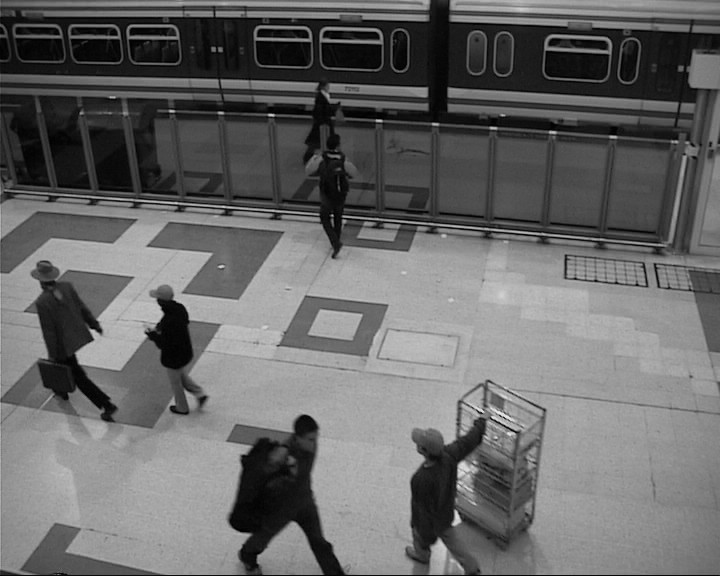
\includegraphics[width=\textwidth]{img/fd-frame.png}
	\end{minipage}
	\hfill
	\begin{minipage}[b]{0.49\textwidth}
		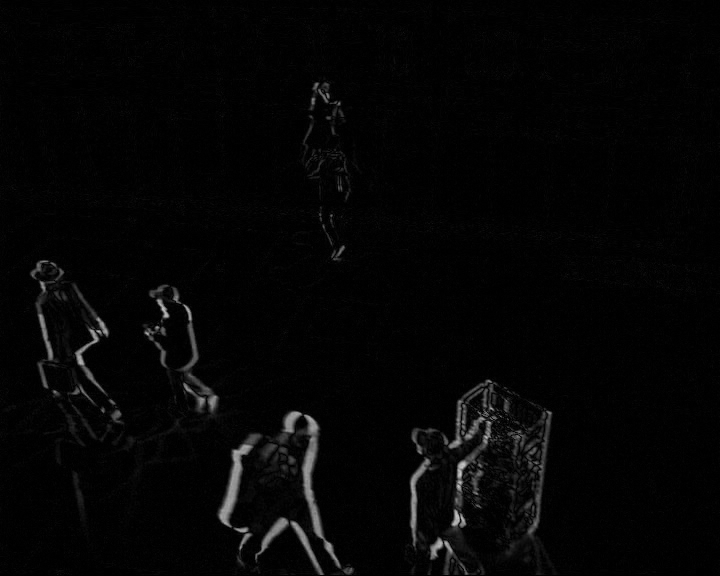
\includegraphics[width=\textwidth]{img/fd-diff.png}
	\end{minipage}
	\caption{Ramka obrazu i wyznaczona różnica ramek.}
	\label{fig:frame-difference-result}
\end{figure}
\section{Moduł generacji tła}

Poza najprostszymi przypadkami analizy ruchu, informacja uzyskana w wyniku odejmowania ramek sekwencji wizyjnej nie jest wystarczająca do analizy strumienia obrazów.
%TODO zdanie do przeredagowania informacja uzyskana w wyniku odejmowanie ramek
% OK
Zagadnienie to może być jednak elementem składowym bardziej rozbudowanych algorytmów, na przykład modułów realizujących algorytm generacji i modelowania tła, czy segmentacji obiektów pierwszoplanowych, gdzie pozwala określić zbiór obiektów będących w ruchu. %TODO i segmentacji obiektów pierwszoplanowych, gdzie pozwala określić, które obiekty są ruchome.
% OK

Generacja tła to zadanie ekstrakcji elementów \textit{tła} badanego obrazu, a więc takich, które stanowią stały, niezmienny element sceny. 
Dzięki wydzieleniu obiektów tła, pozostałe elementy obrazu klasyfikowane są jako obiekty pierwszoplanowe. 
Zwykle, uważa się za nie elementy będące w ruchu. Uwzględnić jednak należy również obiekty, których ruch jest niejednostajny, na przykład zatrzymujący się piesi lub pojazdy na skrzyżowaniu. %TODO no właśnie nie, bo jeszcze są zatrzymne samochodu, piesi itp...
% OK

Bardziej zaawansowane metody generacji tła uwzględniają ponadto dodatkowe warunki klasyfikacji obiektów do dwóch z omawianych grup:
\begin{itemize}
	\item cienie -- choć mogą być związane zarówno z elementami tła jak i pierwszoplanowymi, oczekiwane jest zwykle, by nie były uwzględniane w grupie obiektów wymagających analizy,
	\item ruchome elementy tła -- występujące na przykład pod wpływem wiatru ruchy roślin czy deszcz nie powinny być traktowane jako obiekty pierwszoplanowe,
	\item obiekty o niejednostajnym ruchu -- algorytm powinien klasyfikować poprawnie obiekty pierwszoplanowe, które pojawiają się na scenie a następnie zatrzymują, nie traktując ich jako elementy tła, %TODO nie wiem czy nazwa niejednorodny ruch to jest to o co chodzi...
	% niejednostajny brzmi lepiej
	\item obiekty wzajemnie przesłaniające się -- elementy pierwszego planu mogą, w wyniku ruchu, zostać zasłonięte z perspektywy kamery przez elementy tła. Nie powinno to wpłynąć na zmianę klasyfikacji obiektów z obu grup.
	\item warunki oświetleniowe -- możliwość zmiany warunków oświetleniowych może wymagać ciągłej korekty parametrów generowanego modelu tła. Uwzględnić należy zarówno zmiany długookresowe, wynikające na przykład z cyklu dobowego, jak i krótkookresowe, wynikające z nagłych zmian, takich jak włączenie lub wyłączenie sztucznego oświetlenia sceny.
\end{itemize}

Zagadnienie modelowania tła nie jest trywialne i wymaga metod uwzględniających część lub wszystkie z wymienionych powyżej ograniczeń. 
Opracowanie dostępnej literatury poruszającej ten temat znaleźć można w pracy \cite{Kryjak2012}.
W ramach niniejszego opracowania zdecydowano się na realizację generacji tła przy pomocy metody średniej bieżącej, opisanej zależnością \eqref{eq:background-model}. %TODO raczej metody tzw. średniej bieżącej. i bez modułu
% OK
Wartość modelu tła wyznaczana jest niezależnie dla każdej składowej obrazu.
\begin{equation}
\label{eq:background-model}
b^i(x,y) = \alpha p^i(x,y) + (1-\alpha)b^{i-1}(x,y)
\end{equation}
gdzie:
\begin{conditions}
	x,y & współrzędne piksela, \\
	i & indeks ramki w sekwencji obrazów, \\
	p^i(x,y) & wartość w $i$-tej ramce dla piksela o współrzędnych $(x,y)$, \\
	b^i(x,y) & wartość w $i$-tej ramce dla piksela modelu tła o współrzędnych $(x,y)$, \\
	\alpha & współczynnik bezwładności tła z przedziału $(0, 1]$. \\
\end{conditions}

%TODO a coś o przestrzeni barw ?
%dodałem informację powyżej, YCbCr pojawia się nieco dalej

Wadą przedstawionej metody jest jej wrażliwość na krótkookresowe zmiany oświetlenia.
Jednym ze sposobów eliminacji zakłóceń pojawiających się cyklicznie -- na przykład drgań liści pod wpływem wiatru -- jest wykorzystanie wielu niezależnie wyznaczanych modeli tła.
Stosując kilka modeli, budować można warianty dopasowane do najczęściej występujących przypadków, uporządkowanych według prawdopodobieństwa wystąpienia. 
Przy takim podejściu, obliczenia prowadzone są dla każdego modelu tła niezależnie, wartość nie jest jednak aktualizowana w sytuacji, gdy stan piksela nie jest zbliżony do oczekiwanego, związanego z wybranym modelem.
Jednym z dostępnych rozwiązań jest algorytm GMM (\emph{ang.} Gaussian Mixture Model), wykorzystujący kilka rozkładów prawdopodobieństwa Gaussa. 
%TODO 1. Opis przeredagować jeszcze, bo jest cout niejasny. 2. Napisać, że przykłądem jest GMM.
% OK
W niniejszej pracy nie zdecydowano się na realizację opisanej powyżej metody eliminacji zakłóceń, uzasadniając to zachowaniem czytelności i prostoty implementacji.

Algorytm dostosowano do pracy z sygnałem opisanym w przestrzeni barw \textit{YCbCr}. 
Procedura generacji tła odbywa się niezależnie dla każdej składowej sygnału.
Przyjęto, że aktualizacja wartości modelu tła powinna mieć miejsce wyłącznie w przypadku, jeśli aktualnie badany piksel może być uznany za element tła. 
W tym celu wprowadzono dwa warunki wykonania obliczeń:
\begin{enumerate}
	\item Warunek ruchu.
	
	Aktualizacja powinna mieć miejsce wyłącznie w przypadku, jeśli wartość piksela nie uległa zmianie większej niż dopuszczalna względem poprzedniej ramki obrazu. %TODO styl. coś nie tak ze zdaniem 
	% poprawiłem
	W przeciwnym razie przyjąć można, że nastąpił ruch elementu i piksel nie należy do tła. %TODO raczej, że piksel 
	% OK
	Zależność opisano wzorem \eqref{eq:background-model-movement-mask}.
	
	\begin{equation}
	\label{eq:background-model-movement-mask}
	d^i_Y(x,y) > T_{fd}
	\end{equation}
	gdzie:
	\begin{conditions}
		d^i_Y(x,y) & różnica ramek dla kanału $Y$ obrazu, opisana wzorem \eqref{eq:frame-difference}, \\ %TODO ramek, sekwencji brzmi dziwnie
		% OK
		T_{fd} & próg ruchu z zakresu $[0,255]$, zwykle nie przekraczający $30$. %TODO może po prostu próg ?
		% OK?
	\end{conditions}

	Większe wartości współczynnika $T_{fd}$ pozwalają dokonać aktualizacji modelu tła dla elementów o coraz większej różnicy względem poprzedniej ramki obrazu.
	
	\item Warunek tła.
	
	Aktualizacja powinna mieć miejsce wyłącznie w przypadku, jeśli piksel został sklasyfikowany jako element tła na bazie aktualnego modelu.
	%TODO nie może zostać tylko został
	% OK
	Zależność opisano równaniem \eqref{eq:background-model-background-mask-1}.
	\begin{equation}
	\label{eq:background-model-background-mask-1}
	w_Ym^i_Y(x,y) + w_{Cb}m^i_{Cb}(x,y) + w_{Cr}m^i_{Cr}(x,y) > T_{bg}
	\end{equation}
	%TODO jednak wprowadziłbym tu wagi i potem napisał, że było 1,2,2 w eksperymentach...
	% OK
	gdzie:
	\begin{conditions}
		m^i(x,y) & zmiana wartości piksela względem tła, opisana zależnością \eqref{eq:background-model-background-mask-2}, \\
		w_k & współczynnik wagi związany z $k$-tym kanałem \\
		T_{bg} & współczynnik bezwładności przynależności do tła z zakresu $[0,255]$. \\
	\end{conditions}
	
	\begin{equation}
	\label{eq:background-model-background-mask-2}
	m^i_k(x,y) = | p^i_k(x,y) - b^{i-1}_k(x,y)|
	\end{equation}
	gdzie:
	\begin{conditions}
		k & indeks składowej barwnej sygnału. \\ %TODO indeks składowej barwnej
		% OK
	\end{conditions}
	
	Większe wartości parametru $T_{bg}$ pozwalają na aktualizację modelu tła w sytuacji, gdy różnica piksela względem aktualnego modelu tła jest znaczna. 
	Jego wartość nie przekracza jednak zwykle $30$.
\end{enumerate}

W trakcie eksperymentów przyjęto wartości współczynników wag przynależności do tła odpowiednio: $w_Y=1, w_{Cb} = 2, w_{Cr} = 2$.
Aktualizacja modelu tła powinna mieć miejsce wyłącznie w sytuacji, gdy spełnione są oba warunki przedstawione powyżej.
Schemat blokowy algorytmu przestawiono na rysunku \ref{fig:background-model}.

\begin{figure}[h]
	\centering
	\def\svgwidth{\textwidth}
	\input{img/background-model.pdf_tex}
	\caption{Schemat architektury wyliczającej model tła.}
	\label{fig:background-model}
\end{figure}
%TODO ten schemat jest do modyfikacji, no chyba, że to rzeczywiście sa zupełnie osobne VDMA. Ale i tak moduł odejmowania ramek. Konwersja do YCbCr. wyjście w postai maski, a nie tylko modelu tła..
% dodałem kolejny schemat, na którym czytelniej przedstawiłem szczegóły działania bloku "moduł wyznaczania..."
% dodałem konwersję, ale pozostałe elementy przeniosłem na niezależny schemat

Działanie modułu generacji tła przedstawiono na schemacie \ref{fig:background-model-impl}. Na wejściu, moduł otrzymuje aktualną wartość piksela w przestrzeni barw \textit{YCbCr} oraz poprzednią wartość piksela i modelu tła. Ponadto, przekazywane są parametry opisujące działanie algorytmu: $\alpha$, $T_{bg}$ oraz $T_{fd}$. Moduł odpowiedzialny jest za wyznaczenie maski obiektów tła oraz nowej wartości modelu, które stanowią wyjścia elementu obliczeniowego.

\begin{figure}[h]
	\centering
	\def\svgwidth{\textwidth}
	\input{img/background-model-impl.pdf_tex}
	\caption{Algorytm wyznaczania modelu tła.}
	\label{fig:background-model-impl}
\end{figure}

Algorytm wymaga wykorzystania dwóch buforów AXI VDMA. 
Jeden z nich przeznaczony jest do buforowania ramki obrazu wejściowego, natomiast drugi przechowuje aktualny model tła. 
Alternatywą jest zastosowanie wspólnego bufora i przechowywanie w nim dwóch scalonych sygnałów. Rozwiązanie to pozwala ograniczyć zapotrzebowanie na zasoby logiczne, może jednak wiązać się z trudnościami w synchronizacji wielu strumieni wizyjnych.%TODO a to drugie jest lepsze/gorsze ?
% rozwinąłem nieco

Algorytm zintegrowano z układem umożliwiającym komunikację z procesorem ARM, co pozwala na transmisję uzyskanego modelu tła i jego dalszą analizę. %TODO umoż, umoż..
%OK
Wykorzystano w tym celu trzeci moduł AXI VDMA. %TODO nie ma go na schemacie...
%wg mnie ten moduł nie należy do algorytmu, a jest po prostu narzędziem do transmisji danych, dlatego nie dodałem go do schematu, by nie zmniejszać czytelności
W praktycznych zastosowaniach moduł ten może okazać się zbędny, ze względu na to, że w jednym z pozostałych modułów VDMA przechowywany jest model tła dla poprzedniej klatki obrazu. 
Opóźnienie jednego cyklu nie powinno wpłynąć negatywnie na jakość działania aplikacji. 
Niezależny moduł VDMA pozwala jednak na przesyłanie wyników również w przypadku, gdy algorytm generacji tła nie stanowi ostatniego etapu obliczeń.


Ze względu na duże zapotrzebowanie algorytmu na elementy obliczeniowe logiki reprogramowalnej, zdecydowano się ograniczyć rozmiar kolejek FIFO do $64$ elementów.
Sprawdzono działanie aplikacji dla sygnału wizyjnego o rozdzielczości $1280 \times 720$ pikseli i częstotliwości sześćdziesięciu ramek na sekundę.
Szacowane zapotrzebowanie wynikowego systemu na energię elektryczną nie powinno przekroczyć $1,936W$. Właściwa energia wymagana do przeprowadzania operacji obliczeniowych nie przekracza wartości $1,797W$, w tym $1,565W$ ( $87\%$) to energia wymagana do obsługi układu ARM.


\begin{table}[h]
	\caption{Wykorzystanie zasobów przez aplikację.}
	\centering
	\label{tab;background-model-utilization}
	\begin{tabular}{|l|c|c|c|}
		\hline
		\textbf{Rodzaj zasobu} & \textbf{Użycie} & \textbf{Dostępne} & \textbf{Procent użycia}      \\ \hline
		FF                     & $6938$            & $17600$             & $39,42\%$                 \\ \hline
		LUT 6                  & $13670$            & $17600$             & $77,67\%$                 \\ \hline
		SLICE                  & $4400$            & $4400$             & $100\%$                 \\ \hline
		DSP 48                 & $15$               & $80$                & $18,75\%$                    \\ \hline
		BRAM                   & $12$               & $60$                & $20\%$                   \\ \hline
	\end{tabular}
\end{table}
%TODO na pewno 100 % Slice ?
% tak sądzę. Tzn tak było napisane w raporcie vivado. Moduły VDMA i pokrewne połykają zasoby...
% miałem spore problemy z "upchaniem" trzech VDMA na ZYBO, sądzę że stąd to 100 %

W tabeli \ref{tab;background-model-utilization} przedstawiono zapotrzebowanie na zasoby FPGA układu Zynq.
Proporcjonalnie duże zużycie zasobów wynika z konieczności wykorzystania wielu modułów AXI VDMA oraz innych elementów wykorzystujących interfejs AXI. 
Może ono być ograniczone przez wykorzystanie jednego modułu do obsługi buforowania zarówno ramki obrazu, jak i modelu tła. 
W przypadku złożonych aplikacji, konieczne może okazać się użycie układu z większą liczbą dostępnych zasobów obliczeniowych. %TODO z większą liczbą dostępnych...
% OK
Moduł przeznaczony jest do pracy z częstotliwością $200MHz$, co pozwala na analizę sygnału wideo o rozdzielczości $1920 \times 1080$ pikseli i częstotliwości obrazu $60Hz$.

Wynik działania aplikacji przedstawiono na rysunku \ref{fig:background-model-result}. Projekty Vivado i PetaLinux związane z omawianą aplikacją dodano jako załączniki do pracy oraz udostępniono w repozytorium \cite{git-repository}. Proces konfiguracji aplikacji przedstawiono w rozdziale \ref{sec:background-buffer-conf}.
\begin{figure}[H]
	\centering
	\begin{subfigure}[b]{0.49\textwidth}
		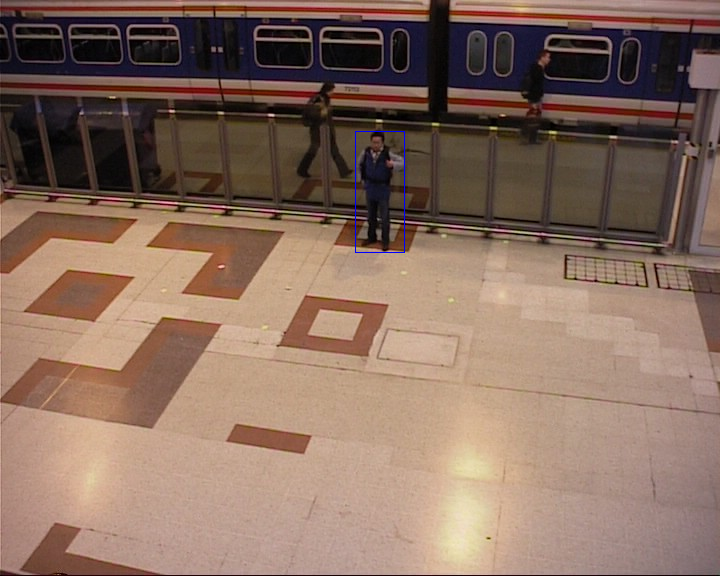
\includegraphics[width=\textwidth]{img/bg-input.png}
		\caption{Ramka obrazu.}
		\vspace{1ex}
	\end{subfigure}
	\hfill
	\begin{subfigure}[b]{0.49\textwidth}
		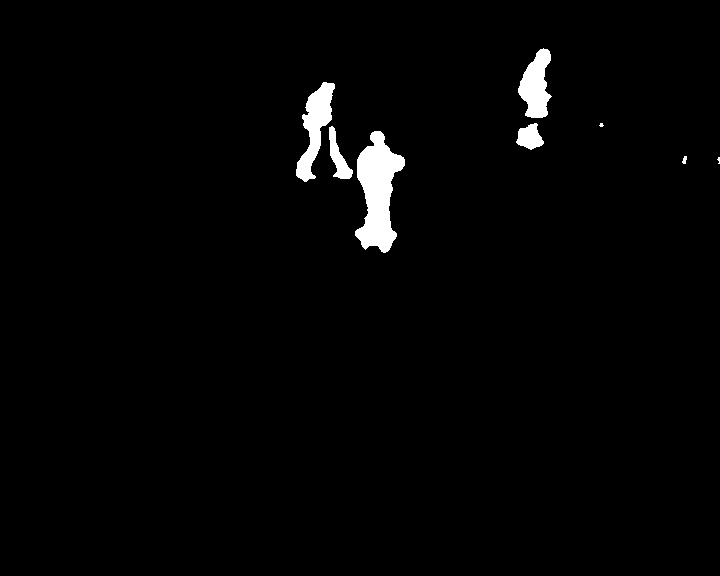
\includegraphics[width=\textwidth]{img/bg-fg.png}
		\caption{Maska obiektów pierwszoplanowych.}
		\vspace{1ex}
	\end{subfigure}

	\begin{subfigure}[b]{0.49\textwidth}
		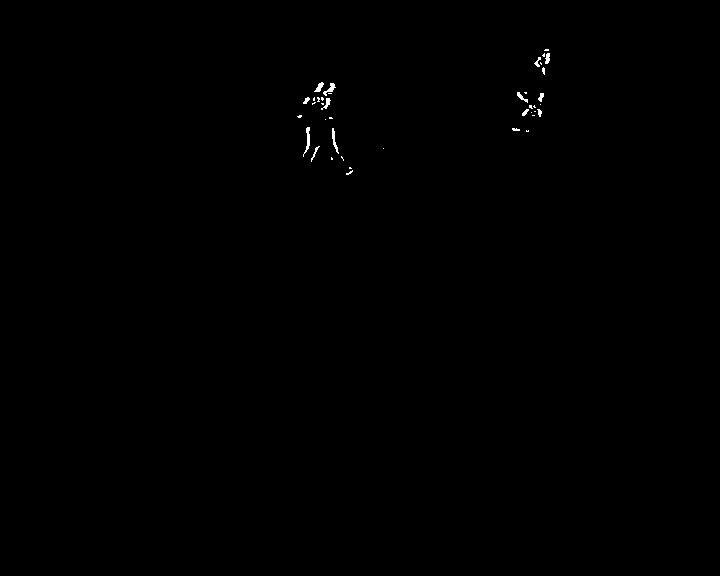
\includegraphics[width=\textwidth]{img/bg-mo.png}
		\caption{Maska ruchu.}
	\end{subfigure}
	\hfill
	\begin{subfigure}[b]{0.49\textwidth}
		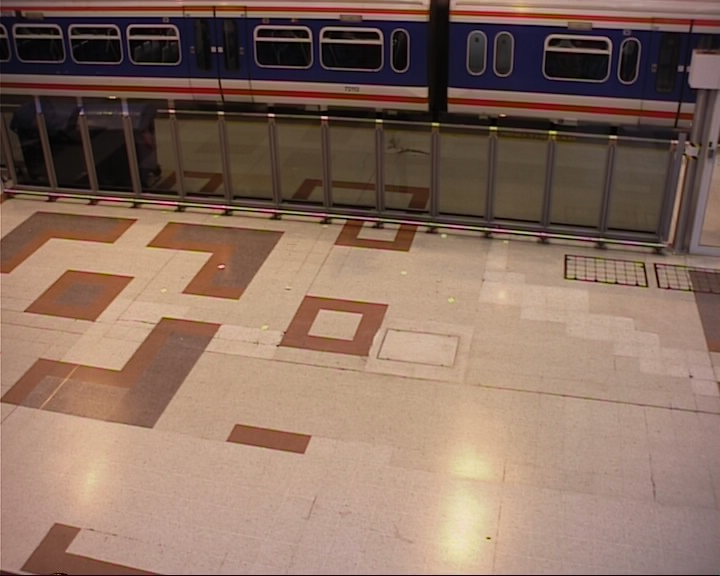
\includegraphics[width=\textwidth]{img/bg-model.png}
		\caption{Model tła.}
	\end{subfigure}
	\caption{Ramka obrazu i wyznaczona różnica ramek.}
	\label{fig:background-model-result}
\end{figure}

Dzięki zastosowaniu maski ruchu, obiekty poruszające się nie wpływają na stan modelu tła. Ponadto, dzięki badanu warunku przynależności do tła, osoba znajdująca się na pierwszym planie i nie będąca w ruchu również nie wpływa negatywnie na wynik działania algorytmu generacji tła.

%TODO 1. Te akapity krótkie - to dotyczy całej pracy, ale przypominam.
% OK
%TODO 2. Uwagi podobnie jak wczęsniej tj.
%TODO może jakieś zdjęcie pokazuję, że działa. No i jeszcze te wszyskie szczegóły konfiguracji tego modułu. I coś o tym źródle - że ma to być film HD. Kolejna kwestia to przygotowanie takiego projektu - działającego/wzorcowego i do repo na płytce, a tu napisać, że takie coś jest.

%TODO Wydaje mi się, że jeszcze umawialiśmy się na przesył maski (kwestię indeksacji pozostawię) i coś po stronie PetaLiunx.
% co do indeksacji, nie sądzę, by moduł "zmieścił" się obok vdma na ZYBO. Musiałbym mocno zoptymalizować te struktury vdma, a wydaje mi się, że cenniejsza jest jednak czytelność tego, co mam teraz. Dlatego nie zająłem się indeksacją po stronie fpga. W CPU to w zasadzie wywołanie jednej metody w CV, ale nie ma szans na real-time.
% rzeczy po stronie peta opisałem w kolejnej sekcji.
% na wyjściu modułu dostępne są wartości maski, zaktualizowałem schemat
\section{Integracja z systemem PetaLinux}

Na etapie prototypowania, elementy logiki reprogramowalnej kontrolowane były przez aplikację działającą w trybie \textit{bare-metal}, bez wsparcia dla systemu operacyjnego.
Po zakończeniu tego etapu, możliwe stało się zaprojektowanie aplikacji działającej pod kontrolą systemu PetaLinux, umożliwiającej wykorzystanie zaawansowanych funkcji systemu.
Założono, że projektowana aplikacja powinna spełniać szereg wymagań:

\begin{itemize}

	\item Konfiguracja modułów AXI i algorytmu.
	
	Podstawowym zadaniem aplikacji powinno być przeprowadzenie wstępnej konfiguracji modułów, wykorzystując w tym celu interfejs AXI. 
	Proces ten powinien mieć miejsce na etapie uruchamiania aplikacji. 
	Aplikacja powinna być też odpowiedzialna za przeprowadzenie procesu konfiguracji parametrów wykonywanego algorytmu wizyjnego.	
	Ponadto, działanie algorytmu nie powinno zostać przerwane w razie wyłączenia programu.
	
	\item Konfiguracja aplikacji przy użyciu argumentów wiersza poleceń.
	
	Konfiguracja parametrów działania aplikacji, w tym rozmiar przetwarzanych obrazów i parametry algorytmu powinny być konfigurowane przy użyciu argumentów wiersza poleceń.
	
	\item Monitorowanie działania algorytmu.
	
	Aplikacja powinna udostępniać opcję monitorowania stanu elementów algorytmu, ze szczególnym uwzględnieniem modułów AXI VDMA, odpowiedzialnych za buforowanie danych oraz komunikację z procesorem.
	
	\item Zapis wyników pracy algorytmu.
	
	Program powinien być odpowiedzialny za zapis wyników działania algorytmu, na przykład w formie obrazów przechowywanych w pamięci.
	
	\item Wykorzystanie komunikacji sieciowej.
	
	Uruchomienie aplikacji nie powinno wymagać fizycznego dostępu do układu Zynq. 
	Docelowym narzędziem komunikacji jest protokół SSH. 
	Ponadto, aplikacja powinna udostępniać interfejs wykorzystujący protokół HTTP, umożliwiający weryfikację stanu aplikacji przy użyciu przeglądarki internetowej.
	
	\item Kompatybilność z procedurami biblioteki OpenCV
	
	Aplikacja powinna zapewniać zgodność z technikami programowania wykorzystywanymi przez bibliotekę OpenCV w stopniu umożliwiającym użycie algorytmów biblioteki ze strukturami danych wykorzystywanymi przez program.
\end{itemize}

Zaprojektowano aplikację w języku C, spełniającą przedstawione wymagania.
Program odpowiedzialny jest za konfigurację elementów logiki reprogramowalnej na podstawie wartości przekazanych przy użyciu argumentów wiersza poleceń. 
Aplikacja wykonuje operacje monitorowania działania algorytmu i zapisu informacji logu do pliku. %TODO powt. odpow
% OK
Ponadto, umożliwia cykliczny zapis obrazów będących wynikiem działania algorytmu do plików graficznych. 

Proces obsługi aplikacji opiera się na wykorzystaniu protokołu SSH, program udostępnia również interfejs HTTP, umożliwiający uzyskanie aktualnych wyników działania algorytmu.
Zbadano możliwość wykorzystania aplikacji w roli elementu obliczeniowego, odpowiedzialnego za przeprowadzenie części operacji algorytmicznych. %TODO powt. obliczeń
% OK
Zaproponowano moduł indeksacji obiektów na bazie generowanego modelu tła. 
W tym celu wykorzystano procedurę \texttt{cv::connectedComponents} dostępną w bibliotece OpenCV. %TODO No właśnie - to może trzeba to gdzieś zasygnalizować. Najlepiej na poczatu rozdziału, gdzie powienien Pan opisać całosć tego interesu... tzn. cały algorytm, scheamt, podział HW/SW itp.
% rozwinąłem na początku rozdziału

Ze względu na ograniczenia sprzętowe, moduł indeksacji nie był w stanie spełnić wymagań pracy w czasie rzeczywistym dla sygnału wizyjnego o częstotliwości $60Hz$ i rozdzielczości $1280 \times 720 $ pikseli -- jego wydajność nie przekraczała piętnastu ramek na sekundę.
Na rysunku \ref{fig:background-buffer-www} przedstawiono widok interfejsu \emph{www} udostępnianego przez aplikację, przedstawiający aktualny stan i wyniki działania programu. Interfejs wyświetla model tła oraz najnowszą ramkę obrazu, a także pokazuje wartości parametrów algorytmu.
Związane z omawianą aplikacją dodano jako załączniki do pracy oraz udostępniono w repozytorium \cite{git-repository}.
\begin{figure}[!htb]
	\centering
	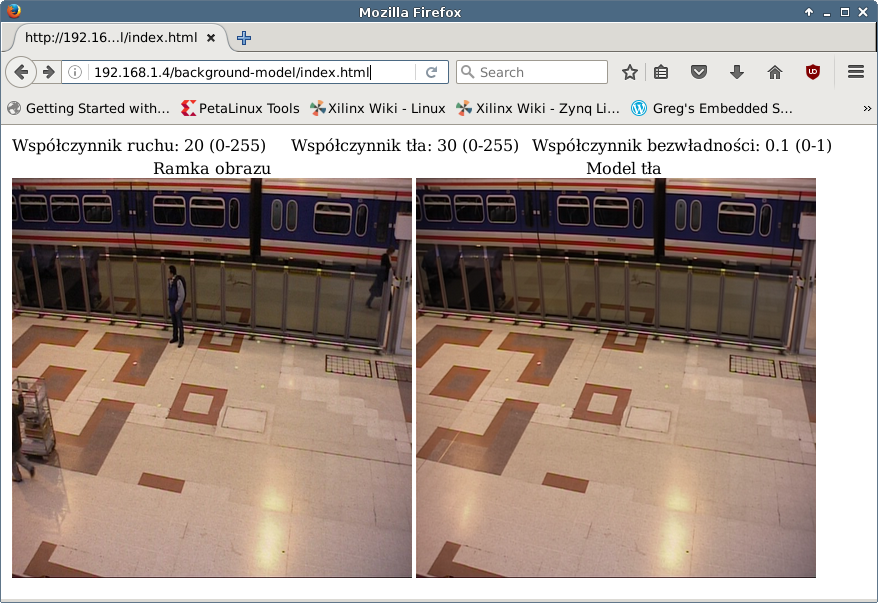
\includegraphics[width=12cm]{img/www-iface.png}
	\caption{Interfejs www aplikacji.}
	\label{fig:background-buffer-www}
\end{figure}
\section*{Podsumowanie}

Zaproponowane rozwiązania projektowe pozwalają na wykorzystanie części funkcji systemu operacyjnego, które badane były w ramach pracy. 
Szczególnie istotnym zagadnieniem jest komunikacja pomiędzy elementami zaprojektowanymi w dwóch architekturach. 
Dzięki wykorzystaniu transmisji danych, możliwe jest zaprojektowanie algorytmów podzielonych na moduły wykonywane naprzemiennie przez obie części układu, wykorzystując atuty obu architektur do możliwie maksymalnego zwiększenia wydajności pełnego algorytmu.

Ponadto, wykorzystanie systemu operacyjnego pozwala na realizację zadań zwykle niemożliwych w przypadku projektu aplikacji realizowanych wyłącznie przy użyciu elementów logiki reprogramowalnej lub sterowanych przez aplikację \textit{bare-metal}. 
Program działający pod kontrolą systemu operacyjnego umożliwia prowadzenie zadań konfiguracji, kontroli i monitorowania działania aplikacji z wykorzystaniem komunikacji sieciowej.

Wykorzystanie systemu operacyjnego pozwala również na implementację aplikacji w dowolnym języku programowania. 
Dzięki temu, stosując dedykowane rozwiązania programistyczne, projektowanie aplikacji o rozbudowanych możliwościach zajmuje mniej czasu.

W trakcie realizacji projektu napotkano szereg ograniczeń. %TODO trochę - styl archite...
% OK
\begin{itemize}
	\item Liczba elementów obliczeniowych wykorzystywanego układu Zynq nie pozwala na realizację rozbudowanych rozwiązań algorytmicznych przy użyciu zaproponowanych technik. 
	Ze względu na duże zapotrzebowanie na elementy logiki przez moduły AXI VDMA, buforowanie pełnych ramek obrazu jest kosztowne. 
	W przypadku bardziej rozbudowanych algorytmów, konieczne może być wykorzystanie układu o większych możliwościach lub zastosowanie technik optymalizacji zużycia zasobów.
	
	\item Procesor ARM dostępny w układzie Zynq nie pozwala na realizację algorytmów wizyjnych o dużej złożoności obliczeniowej w  czasie rzeczywistym. 
	Próba wykorzystania rozwiązań biblioteki OpenCV do indeksacji obiektów pierwszoplanowych nie spełniała ograniczeń czasowych dla sygnału o częstotliwości $60Hz$.
	
	W przypadku bardziej złożonych algorytmów, konieczne może być wykorzystanie układu o większej wydajności. 
	Innym rozwiązaniem może być użycie protokołów sieciowych do transmisji danych do elementu obliczeniowego oferującego wydajność wystarczającą do realizacji zadań obliczeniowych. 
	Dla zbioru algorytmów, których realizacja strumieniowa jest znana, możliwe jest również przeniesienie zadań obliczeniowych do elementów logiki reprogramowalnej. 
	W przypadku, gdy żadne z zaproponowanych rozwiązań nie jest możliwe, konieczne jest ograniczenie częstotliwości działania algorytmu do poziomu, dla którego układ obliczeniowy będzie spełniać ograniczenia czasowe.
	
	\item Proces budowy systemu operacyjnego na bazie projektu sprzętowego jest złożony i wymaga dużych nakładów czasowych. 
	Z tego powodu, na etapie projektowania połączeń logiki reprogramowalnej, wykorzystanie aplikacji typu \textit{bare-metal} pozwala skrócić okres prototypowania.
	
	W konsekwencji, konieczne może być zaprojektowanie dwóch aplikacji związanych z projektem: aplikacji \textit{bare-metal}, wykorzystywanej na etapie prototypu oraz programu działającego pod obsługą systemu operacyjnego, projektowanego po ukończeniu implementacji sprzętowej.
	
	Z tego powodu, aplikacje systemu operacyjnego nie pozwalają w pełni zastąpić programów \textit{bare-metal} i powinny być traktowane jako metoda rozbudowy możliwości projektu.
\end{itemize}

%TODO Tak samo jakieś screeny.
%TODO No i co z tego, że indeksacja 15 fps - a da się to jakoś pokazać ? Że to działa ? Wizualnie.
%TODO Co z HTTP ? 
% http -działa. Dołączę screen interfejsu, choć to będzie coś bardzo prostego. Tzn np aktualny wynik generacji tła czy indeksacji + gdzieś obok wartości parametrów algorytmu. Do tej pory zadowalałem się tym, że gdy uderzałem pod IP ZYBO dostawałem w odpowiedzi png z aktualnym stanem vdma, dlatego nie dodawałem tego do pracy.
% Myślałem o tym, by umożliwić modyfikację parametrów z poziomu http, ale serwer, który napisałem siedzi w C i podejrzewam, że dodanie obsługi parametrów zapytania będzie uciążliwa.

\chapter{Podsumowanie}
\label{chap:summary}

%TODO No tutaj to trzeba się nieco bardziej postarać. 1. Ta formuła "autor" mi się nie podobna. 2. Nie robiłbym z tego kolejnego spisu zawartości, oczyiwście ref mogą zostać, ale struktura pownnina być inna. 3. Po pownej lekturze (przy poprawkach) na pewno będzie łatwiej wybrać najważniejsze osiągnięcia. 4. Nad tymi kierunkami rozwoju też bym poprawcował jeszcze...
% przeregadowałem

Celem niniejszej pracy była analiza możliwości systemu operacyjnego PetaLinux uruchomionego na układzie z~rodziny Zynq i próba wykorzystania go w zagadnieniach związanych z wbudowanymi systemami wizyjnymi. 
Użycie systemu operacyjnego oferuje większy, względem aplikacji typu \textit{bare-metal}, zasób możliwości -- w tym komunikację sieciową, metody przechowywania danych, a także realizację zaawansowanych zadań algorytmicznych, dzięki zastosowaniu zewnętrznych bibliotek. %TODO realizację zaawans...
% OK

W ramach pracy zbadano możliwości wykorzystania istniejących systemów operacyjnych do działania na badanej platformie. Omówiono wady i zalety każdego ze znanych autorowi rozwiązań. Poruszono również zagadnienie realizacji obliczeń w czasie rzeczywistym w układzie Zynq. Zagadnienia te zebrano w rozdziale \ref{cha:platform}.

Kolejnym krokiem było opracowanie funkcjonalności, które mogą znaleźć zastosowanie w projektach realizujących zadania przetwarzania obrazów i sekwencji wizyjnych. Zebrano informacje teoretyczne oraz wnioski z zastosowań praktycznych protokołu AXI oraz wyjaśniono jego rolę w projektowaniu współczesnych układów obliczeniowych, realizowanych na platformie Zynq.
Wyniki analizy teoretycznej oraz wnioski uzyskane na etapie projektowania implementacji zebrano w rozdziale \ref{cha:functionalities}. 

Na podstawie informacji zebranych w dwóch wymienionych rozdziałach, zaproponowano metodę realizacji algorytmu generacji tła w logice reprogramowalnej. Wynik działania modułu był następnie transmitowany do pamięci operacyjnej procesora ARM przy użyciu mechanizmu AXI VDMA. Aplikacja działająca pod kontrolą systemu PetaLinux była odpowiedzialna za końcową analizę obrazu i archiwizację wyników.
W ramach realizacji projektu zaproponowano metodę buforowania pełnej ramki obrazu przy użyciu modułu AXI VDMA. Zaprojektowano również moduł wyznaczający różnicę dwóch kolejnych klatek obrazu, który może stanowić element składowy rozbudowanych systemów wizyjnych.
W trakcie realizacji projektu napotkano na ograniczenia, w tym niewystarczającą ilość zasobów logicznych oraz niewielką wydajność procedur algorytmicznych uruchamianych na procesorze ARM, w wyniku których nie zbudowano kompletnego systemu wizyjnego wykorzystującego proponowane techniki.
Opis projektu i wnioski z jego realizacji zebrano w rozdziale \ref{cha:project}.

Zebrano również informacje związane z praktycznym wykorzystaniem omawianych funkcjonalności w projektach wizyjnych. Przedstawiono metody konfiguracji kolejnych modułów w ujęciu ogólnym, możliwe do wykorzystania w trakcie projektowania rozwiązań algorytmicznych na dowolną kartę rodziny Zynq. Informacje te znaleźć można w rozdziale \ref{cha:vivado-conf}.

Materiał zebrany i przedstawiony w ramach niniejszej pracy może posłużyć za podstawę do realizacji zaawansowanych algorytmów wizyjnych z wykorzystaniem platformy Zynq i systemu operacyjnego PetaLinux. 
Przedstawione techniki mogą zostać wykorzystane do rozwoju istniejących, jak i projektowania nowych aplikacji.

Zbiór przedstawionych w ramach pracy technik nie wyczerpuje możliwości badanego systemu operacyjnego. 
W ujęciu ogólnym, PetaLinux, lub inny system operacyjny działający na układzie z rodziny Zynq, pozwala na projektowanie aplikacji, które różnią się w znacznym stopniu od programów wykorzystywanych w systemach wbudowanych o ograniczonych możliwościach. 
Zastosowanie zaawansowanych technik projektowania aplikacji pozwali na uzyskanie efektu zbliżonego do programów stosowanych w życiu codziennym, na przykład dzięki wykorzystaniu protokołów komunikacji sieciowej.
Innym kierunkiem rozwoju może być zastosowanie systemów czasu rzeczywistego we współpracy z klasycznym systemem operacyjnym do realizacji obliczeń algorytmicznych z uwzględnieniem rygoru czasowego.

Zaproponowany moduł generacji tła może być dalej rozbudowywany i wykorzystywany w złożonych aplikacjach realizowanych na platformie Zynq.
Zbiór funkcjonalności badanych w ramach pracy nie wyczerpuje możliwości dostępnych w systemie PetaLinux i pokrewnych. Dalszy rozwój badań może pozwolić na zwiększenie praktyczności użycia systemu do realizacji zadań przetwarzania obrazów dzięki zdefiniowaniu obszernego zbioru zasobów możliwych do wykorzystania na etapie projektowania aplikacji.

%TODO Przed tymi istniejącymy dodatkami jeszcze dodatek A - spis zawartości CD.
%TODO Spis treści przed dodatki.
% OK, dodałem dodatek, treść wypełnię później
% pracę sformatowałem zgodnie z tym, co znalazłem w zasadach dyplomowania.
% przenieść spis przed dotatki?
\addcontentsline{toc}{chapter}{Podsumowanie}
\appendix
\chapter*{Dodatki}
\addcontentsline{toc}{chapter}{Dodatki}
\renewcommand{\thesection}{\Alph{section}}

\chapter{Proces konfiguracji modułów logiki programowalnej i systemu operacyjnego PetaLinux}
\label{cha:vivado-conf}

%TODO Kiepski tytuł dla rodziąłu - mało mówi o jego treści.
%TODO Dla całego rodziału - za krótkie akapity
% OK

Użycie funkcjonalności opisywanych w niniejszej pracy wymaga przeprowadzenia konfiguracji wykorzystywanych modułów logicznych oraz systemu operacyjnego. 
W poniższych podrozdziałach zebrano informacje związane z poruszanymi zagadnieniami. Przedstawiono proces konfiguracji bazowego projektu Vivado i wykorzystania go na etapie budowy systemu PetaLinux, a także omówiono proces użycia modułów AXI i wybranych funkcjonalności systemu PetaLinux -- obliczeń równoległych, biblioteki OpenCV, mechanizmu przerwań systemowych. Przedstawiono również proces konfiguracji modułu generacji tła zaproponowanego w rozdziale \ref{cha:project}.%TODO bardziej konkretnnie
% OK

Omawiane zagadnienia wymagają użycia oprogramowania Vivado \cite{vivado-home} i zintegrowanego z nim środowiska programistycznego Xilinx SDK \cite{xsdk-home}. Ponadto, konfiguracja systemu operacyjnego odbywa się przy użyciu narzędzi pakietu PetaLinux Tools \cite{petalinux-tools}.

\section{Podstawowa konfiguracja projektu}

Wykorzystana w projekcie karta -- Digilent ZYBO -- nie jest bezpośrednio wspierana przez środowisko Vivado. %TODO karta
% OK
Wynika z tego konieczność sprecyzowania parametrów układu na etapie tworzenia projektu. 
W trakcie modyfikowania projektu, w przypadku dodania modułów wykorzystujących interfejs wejścia/wyjścia, konieczna jest również konfiguracja parametrów interfejsu. 
Aby uprościć proces projektowania, zalecane jest skonfigurowanie obsługi układu przed utworzeniem projektu. 
Proces ten opisano w dokumentacji producenta \cite{zybo-in-vivado}.

\subsection{Vivado}
\label{sec:vivado-conf}
Utworzyć należy projektu typu \emph{,,RTL Project''}, z odznaczoną opcją \emph{,,Do not specify sources at this time''}.
W kroku \emph{,,Add Constraints''} dodać należy plik konfiguracyjny dla wybranego układu. 
W przypadku ZYBO, plik ten jest dostępny na stronie producenta. 
W kolejnym kroku możliwe jest skonfigurowanie parametrów układu. 
Wykorzystać do tego należy zakładkę \emph{,,Boards''} i wybrać wykorzystywany model.

Po utworzeniu projektu, skonfigurować należy właściwą przestrzeń roboczą dla projektu, wykorzystując do tego opcję \emph{,,IP Integrator --> Create Block Design''}.
Do nowo utworzonej przestrzeni dodać należy moduł IP reprezentujący procesor ZYNQ -- \emph{,,ZYNQ7 Processing System''}.
W kolejnych krokach należy dokonać konfiguracji modułu procesora, klikając dwukrotnie na moduł.

\begin{itemize}
	\item Kanały interfejsu AXI mogą być konfigurowane przez zakładkę \emph{,,PS-PL Configuration''}. Możliwa jest aktywacja kanałów ogólnego przeznaczenia (\emph{GP}) oraz wysokiej wydajności (\emph{HP}).
	
	\item Interfejsy komunikacji konfigurowane mogą być z poziomu zakładki \emph{,,MIO Configuration''}. Zalecane jest aktywowanie interfejsów \emph{ENET 0}, \emph{SD 0} i \emph{UART 1} ze względu na ich wykorzystanie na dalszym etapie pracy.
	
	Przykład konfiguracji interfejsów wejścia/wyjścia przedstawiono na rysunku \ref{fig:vivado-mio-configuration}.
	\begin{figure}[ht]
		\centering
		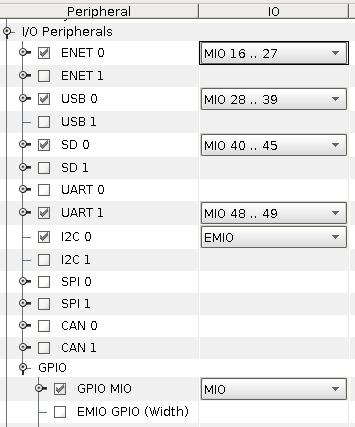
\includegraphics[height=8cm]{img/vivado/mio-configuration.png}
		\caption{Okno konfiguracji interfejsów wejścia i wyjścia.}
		\label{fig:vivado-mio-configuration}
	\end{figure}
	
	\item Parametry sygnałów zegarowych dostępnych z poziomu układów logiki reprogramowalnej modyfikować można w zakładce \emph{,,Clock Configuration/PL Fabric Clocks''}. W projekcie projekcie wymagającym obsługi AXI VDMA wykorzystano trzy sygnały zegarowe:
	\begin{itemize}[label=\textbullet]
		\item bazowy, o częstotliwości $100$MHz,
		\item wykorzystywany do komunikacji interfejsem AXI, o częstotliwości $140$MHz,
		\item zegar obsługi sekwencji wizyjnej, o częstotliwości $200$MHz, umożliwiający współpracę ze strumieniem wideo o częstotliwości $60$Hz i rozdzielczości co $1920 \times 1080$ pikseli.
	\end{itemize}
	
	\item Częstotliwość pracy procesora oraz pamięci zmienić można w zakładce \emph{,,Clock Configuration/Processor/Memory Clocks''}. Zdefiniować należy częstotliwość pracy CPU równą $650$MHz oraz DRR równą $525$MHz.

	%TODO Jakie mają być te częstotliwości ?
	% dodałem
\end{itemize}

Po ukończeniu etapu konfiguracji procesora i powrocie do głównego okna programu, należy użyć opcji \emph{,,Run Block Automation''}. 
Utworzone zostaną połączenia interfejsów pamięci \texttt{DDR} oraz \texttt{FIXED\_IO}.
W przypadku zdefiniowania interfejsów AXI, połączyć należy właściwe sygnały zegarowe. 
Przykład wynikowej konfiguracji projektu przedstawiono na rysunku \ref{fig:vivado-config-result}.

	\begin{figure}[ht]
		\centering
		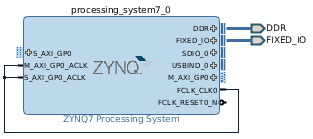
\includegraphics[]{img/vivado/vivado-config-result.png}
		\caption{Okno projektu.}
		\label{fig:vivado-config-result}
	\end{figure}
	
Przedstawiona konfiguracja stanowi podstawę każdego projektu wykorzystującego moduł procesora Zynq.
Po zakończeniu konfiguracji, wygenerować należy warstwę HDL, korzystając z opcji \emph{,,Create HDL Wrapper''} dostępnej po kliknięciu prawym przyciskiem myszy na utworzony wcześniej plik źródłowy.
Skonfigurowany w ten sposób projekt może być budowany i uruchamiany na platformie Zybo.

\subsection{SDK}

W celu utworzenia projektu aplikacji w SDK, konieczne jest wyeksportowanie plików opisujących projekt z poziomu Vivado, wykorzystując do tego opcję \emph{,,File/Export/Export Hardware''} z zaznaczoną opcją \emph{,,Include bitstream''}.
W efekcie, dostępny powinien być projekt \texttt{\textit{nazwa\_projektu}\_hw\_platform\_0}, zawierająca plik \texttt{nazwa\_projektu.hdf}, zawierający konfigurację sprzętową, stanowiący podstawę każdego budowanego programu \textit{bare-metal}. %TODO to jest aplikacja, czy konfiguracja sprzętowa ?
%OK, poprawiłem

W przypadku budowania aplikacji na platformę PetaLinux, na etapie tworzenia projektu, zmodyfikować należy pole \emph{,,OS Platform''} na wartość \emph{,,linux''}, \emph{,,Processor Type''} na \emph{,,ps7\_cortexa9''} oraz wybrać właściwy język programowania.
Tak zdefiniowana aplikacja nie może korzystać z bibliotek udostępnianych przez firmę \emph{Xilinx} )(na przykład zawierających procedury obsługi modułów VDMA czy kontrolera przerwań), ale mogą korzystać z pełnej biblioteki standardowej jeżyka \emph{C} oraz rozszerzeń \emph{POSIX}, w tym operacji wejścia/wyjścia, komunikacji sieciowej czy bibliotek matematycznych.
%TODO zdanie niejasne
% przeredagowałem

W celu uruchomienia aplikacji systemowej na platformie ZYBO, przeprowadzić należy proces budowania i skopiować wynikowy plik z katalogu \texttt{Debug} lub \texttt{Release} do systemu plików systemu PetaLinux. 
Wykorzystać można do tego narzędzie SSH:

\begin{lstlisting}[breaklines=true]
scp Debug/hello-world.elf root@adres-ip:~/
\end{lstlisting}

Aplikację uruchomić można przy użyciu konsoli użytkownika, również stosując narzędzie SSH.

\subsection{PetaLinux}
\label{sec:petalinux-config}

%TODO - a tu nie trzeba zrobić czegoś wcześniej ? Pobrać zainstalowć itp ?
% nie opisywałem procesu instalacji Vivado, uznałem więc, że nie ma też powodu by opisywać instalację petalinux. Dodam na początku rozdziału informację o wykorzystywanych narzędziach

Utworzenie struktury katalogów projektu wykonywane jest przy użyciu poniższego polecenia.

\begin{lstlisting}[breaklines=true]
petalinux-create -t project --template zynq --name (*@\textit{nazwa-projektu}@*)
cd (*@\textit{nazwa-projektu}@*)
\end{lstlisting}

Powstała struktura zintegrowana jest z systemem kontroli wersji \emph{git}, co pozwala zachować uporządkowanie danych wewnątrz projektu oraz wersjonowanie. 
Kolejnym krokiem jest zaimportowanie projektu \emph{Vivado}.

\begin{lstlisting}[breaklines=true]
petalinux-config --get-hw-description=(*@\textit{/sciezka/do/projektu/projekt.sdk/}@*)
\end{lstlisting}

Jeśli polecenie wywołane zostało po raz pierwszy dla danego projektu, uruchomione zostanie narzędzie konfiguracyjne, domyślne ustawienia są jednak poprawne.
Konfiguracja projektu odbywa się przy użyciu polecenia \texttt{petalinux-config}.
Skonfigurować należy metodę uruchamiania systemu -- w omawianym przypadku, uruchomienie następuje na bazie plików znajdujących się na karcie SD.
\begin{lstlisting}[breaklines=true]
petalinux-config
Image Packaging Configuration -> Root filesystem type -> SD card
\end{lstlisting}

Należy również zmodyfikować argumenty przekazywane systemowi na etapie uruchamiania, umożliwiając wykorzystanie sterowników do modułów logiki reprogramowalnej.

\begin{lstlisting}[breaklines=true]
petalinux-config
Kernel Bootargs -> dezaktywować opcję Generate boot args automatically i zdefiniować własną wartość
console=ttyPS0,115200 earlyprintk uio_pdrv_genirq.of_id=generic-uio root=/dev/mmcblk0p2 rw rootwait 
\end{lstlisting}
Następnie, przeprowadzić należy proces budowania systemu oraz wygenerować pliki wynikowe.

\begin{lstlisting}[breaklines=true]
petalinux-build
petalinux-package --boot --fsbl images/linux/zynq_fsbl.elf --fpga images/linux/system_wrapper.bit --u-boot --force
petalinux-package --image -c rootfs --format initramfs
\end{lstlisting}

Uruchomienie systemu wymaga przygotowania karty SD -- musi ona posiadać dwie partycje, pierwszą, z etykietą \emph{boot} i systemem plików \emph{fat32}, drugą -- odpowiednio \emph{sys} i \emph{ext4}. 
Pierwsza z nich, zawierająca pliki wymagane na etapie inicjalizacji systemu, musi być poprzedzona 4 MB niezaalokowanej przestrzeni i mieć rozmiar co najmniej 40 MB. 
Druga partycja zawiera pliki systemowe, jej rozmiar powinien wynosić co najmniej kilkaset megabajtów. 
Proces formatowania przeprowadzić można przy użyciu narzędzia \emph{gparted}. Na rysunku \ref{fig:gparted-screen} przedstawiono efekt konfiguracji karty SD.
%TODO może screen z gparted jak to wygląda.
% OK

\begin{figure}[H]
	\centering
	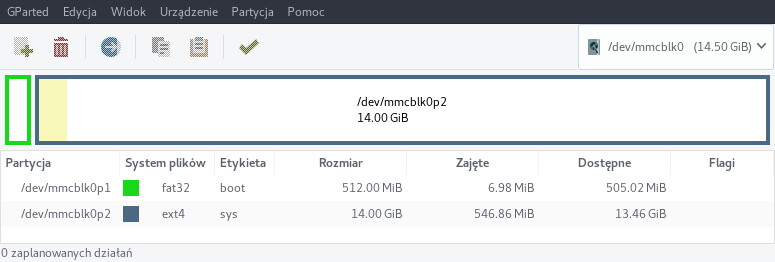
\includegraphics[width=12cm]{img/gparted-screen.png}
	\caption{Partycjonowane karty SD przy użyciu programu gparted.}
	\label{fig:gparted-screen}
\end{figure}

Pliki wynikowe należy przenieść na kartę SD, korzystając z poniższych poleceń.

\begin{lstlisting}[breaklines=true]
rm -rf /(*@\textit{punkt-montowania}@*)/sys/*
cp images/linux/BOOT.BIN /(*@\textit{punkt-montowania}@*)/boot/
cp images/linux/image.ub /(*@\textit{punkt-montowania}@*)/boot/
cp images/linux/rootfs.cpio /(*@\textit{punkt-montowania}@*)/sys/
cd /(*@\textit{punkt-montowania}@*)/
pax -rvf rootfs.cpio
sync
cd -
\end{lstlisting}

Ze względu na mechanizm buforowania przez kontroler operacji zapisu danych, pamiętać należy o wywołaniu polecenia \texttt{sync}, zapewniającego zachowanie integralności danych.

Karta SD pozwala na uruchomienie systemu operacyjnego na układzie i przechowywanie danych użytkownika pomiędzy startami układu. 
Dalsza praca z systemem odbywać się może przez protokoły komunikacji \emph{SSH} lub \emph{UART}.

\section{Konfiguracja modułu wykorzystującego interfejs AXI}
\label{sec:vivado-axi-dma}

%TODO 1-2 zdania wstępu
% OK
Interfejs AXI stanowi podstawową metodę komunikacji pomiędzy modułami logiki programowalnej oraz elementami FPGA i CPU. Dzięki wykorzystaniu tego protokołu do obsługi projektowanych narzędzi, możliwe jest użycie zbioru elementów dostępnych w bibliotece Vivado i uproszczenie procesu projektowania procedur komunikacyjnych. Poniżej przedstawiono kroki konfiguracyjne wewnątrz narzędzi Vivado i PetaLinux.

\subsection{Vivado}
Oprogramowanie Vivado umożliwia zbudowanie modułu wykorzystującego protokół AXI przez użycie opcji \emph{,,Create and package new IP...''}, zawartej w menu \emph{Tools}.
Na ekranie wyboru zadania wybrać należy opcję \emph{,,Create a new AXI4 peripheral''}.
Po zdefiniowaniu podstawowych danych związanych z modułem, takich jak jego nazwa i nazwisko autora, w kolejnym kroku możliwe będzie zdefiniowanie interfejsu modułu. 
Na tym etapie konfiguracji dodać należy wszystkie połączenia wykorzystujące interfejs AXI. %TODO ????
% OK?
W przypadku modułu konfiguracyjnego o podstawowej strukturze, interfejs zawierać powinien jedno połączenie wykorzystujące protokół AXI w wersji \emph{Lite}, działający w trybie \emph{slave}, z oczekiwaną liczbą rejestrów. 
Każdy rejestr powinien być związany z jedną wartością, której konfiguracja ma być możliwa. 
Przykład konfiguracji przedstawiono na rysunku \ref{fig:axi-dma-interfaces-conf}.
%TODO jest Pan pewnien, że taki moduł to DMA ?
% xilinx nazywa takie moduły axi dma peripherial, to trochę mylące względem właściwego modułu AXI DMA. Sprecyzuję to jakoś...

\begin{figure}[H]
	\centering
	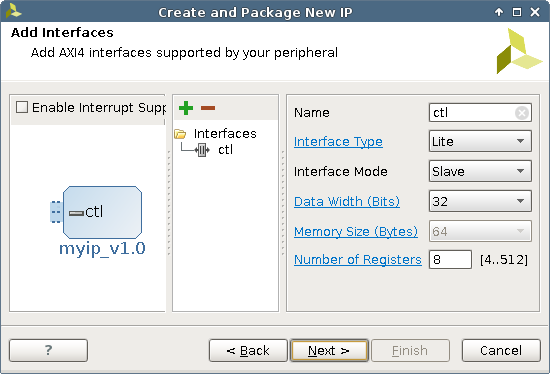
\includegraphics[width=8cm]{img/vivado/axi-dma-interfaces-conf.png}
	\caption{Konfiguracja interfejsów modułu AXI DMA.}
	\label{fig:axi-dma-interfaces-conf}
\end{figure}

W omawianym przykładzie zdefiniowano interfejs AXI o nazwie \emph{ctl}, związany z ośmioma rejestrami o długości trzydziestu dwóch bitów w pamięci.
Zdefiniowanie interfejsów kończy proces podstawowej konfiguracji modułu. W kolejnym kroku należy wybrać opcję \emph{,,Edit IP''} w celu dostosowania kodu źródłowego modułu.

Po wygenerowaniu, z modułem powinien być związany jeden plik źródłowy, zwierający instrukcje odpowiadające za obsługę komunikacji przy użyciu interfejsu AXI.
Do pliku dodać należy elementy odpowiedzialne za zdefiniowanie wyjść modułu oraz przypisanie im właściwych wartości.
W celu zadeklarowania wyjść modułu, odpowiadające im wpisy należy umieścić po komentarzu \emph{,,// Users to add ports here''}. Przykład przedstawiono na listingu \ref{listing:axi-dma-outputs}. %TODO powt. zdefinowane
% OK

\begin{lstlisting}[breaklines, label=listing:axi-dma-outputs, caption=Definicja interfejsów wyjściowych modułu.]
// Users to add ports here
output wire parameter_a,
output wire [7:0] parameter_b,
output wire [15:0] parameter_c,
output wire [31:0] parameter_d,
// User ports ends
\end{lstlisting}

Zdefiniowano cztery sygnały wyjściowe, o różnej liczbie bitów.
Następnie, należy dokonać modyfikacji kodu odpowiedzialnego za powiązanie wartości parametrów z rejestrami modułu. 
Rejestry AXI zdefiniowane są poniżej linii \emph{,,//-- Number of Slave Registers N''}, gdzie \emph{N} to liczba dostępnych rejestrów. Rejestry te mają nazwy \texttt{slv\_reg\emph{n}}, gdzie \emph{n} to indeks rejestru -- nie jest zalecana modyfikacja tych nazw.
Modyfikacji kodu należy dokonać poniżej linii \emph{,,// Add user logic here''}. 
Przykład przedstawiono na listingu \ref{listing:axi-dma-associate}.

\begin{lstlisting}[breaklines, label=listing:axi-dma-associate, caption=Powiązanie wyjść z rejestrami modułu.]
// Add user logic here
assign parameter_a = slv_reg0[0];
assign parameter_b = slv_reg1[7:0];
assign parameter_c = slv_reg2[15:0];
assign parameter_d = slv_reg3[31:0];
// User logic ends
\end{lstlisting}

Wartości parametrów powiązano bezpośrednio z danymi znajdującymi się w rejestrach. %TODO powt. przed
% OK?
W rozbudowanych aplikacjach może być konieczne dodanie instrukcji modyfikujących wartości rejestrów przed przesłaniem ich na wyjście modułu.
Po ukończeniu modyfikacji modułu, konieczne jest zapisanie zmian i wygenerowanie plików wynikowych. 
W tym celu należy wykorzystać okno \emph{,,Package IP''}, sekcję \emph{,,Review and Package''}. 
Widok narzędzia przedstawiono na rysunku \ref{fig:axi-dma-review-package}.

\begin{figure}[ht]
	\centering
	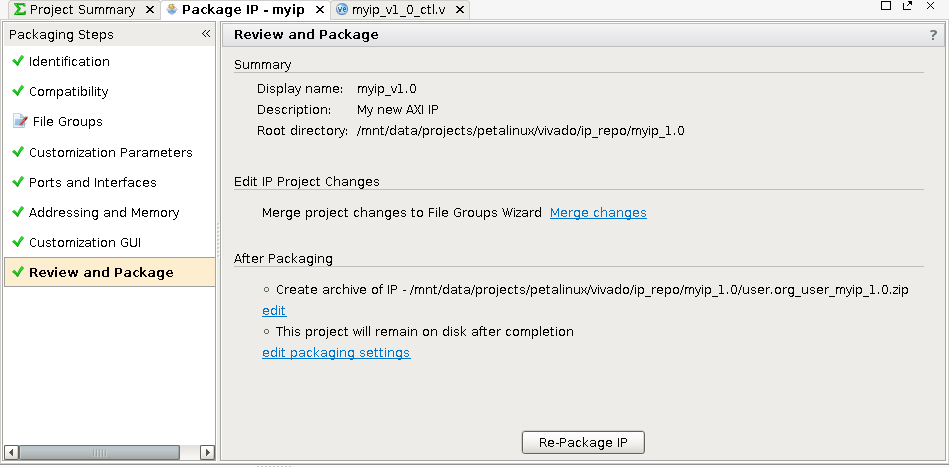
\includegraphics[width=12cm]{img/vivado/axi-dma-review-package.png}
	\caption{Okno finalizacji modyfikacji modułu.}
	\label{fig:axi-dma-review-package}
\end{figure}

Należy wybrać opcję \emph{,,Merge changes''}, umożliwiającą zintegrowanie wprowadzonych zmian z projektem bazowym. 
Następnie, można zakończyć edycję projektu przez wybór opcji \emph{,,Re-Package IP''}. 
Moduł będzie dostępny z poziomu interfejsu wyszukiwania modułów IP.
Dodanie modułu do projektu wymaga zdefiniowania adresu pamięci z nim związanego. Wykorzystać do tego należy okno \emph{,,Address Editor''}, dostępną w z poziomu głównego okna projektu. W omawianym przykładzie, z modułem powiązano przestrzeń rozpoczynającą się od adresu \texttt{0x43000000} i długości \texttt{64K}.
\subsection{SDK}
\label{sec:vivado-axi-dma-sdk}

Konfiguracja wartości parametrów modułu opiera się na zapisie pod właściwe adresy pamięci. %TODO nie lepiej pod właściwy adres w pamięci ?
% OK
W przypadku pracy w trybie \textit{bare-metal}, wykorzystać można instrukcję \emph{Xil\_Out32} z biblioteki \emph{xil\_io.h}. 
W przypadku pracy z systemem PetaLinux, wykorzystać należy biblioteki systemowe. 
Implementację\textit{ bare-metal} przedstawiono na listingu \ref{lis:axi-dma-bare-metal}, natomiast systemową na listingach \ref{lis:axi-dma-petalinux-main}, \ref{lis:axi-dma-petalinux-axi-h} i \ref{lis:axi-dma-petalinux-axi-c}.

\begin{lstlisting}[breaklines, language=C, label=lis:axi-dma-bare-metal, caption=Obsługa modułu w trybie bare-metal.]
#include "xparameters.h"
#include "platform.h"
#include "xil_io.h"

#define PARAMETER_A_REGISTER 0
#define PARAMETER_B_REGISTER 4
#define PARAMETER_C_REGISTER 8
#define PARAMETER_D_REGISTER 12

#define BASEADDR XPAR_ALGORITHM_PARAMETERS_0_CTL_BASEADDR

int main()
{
	init_platform();
	
	Xil_Out32(BASEADDR + PARAMETER_A_REGISTER, 1);
	Xil_Out32(BASEADDR + PARAMETER_B_REGISTER, 25);
	Xil_Out32(BASEADDR + PARAMETER_C_REGISTER, 1 << 10);
	Xil_Out32(BASEADDR + PARAMETER_D_REGISTER, 1 << 30);
	
	while(1);
}
\end{lstlisting}


\begin{lstlisting}[breaklines, language=C, label=lis:axi-dma-petalinux-main, caption=Obsługa modułu w trybie systemowym - \texttt{main.c}.]
#include <fcntl.h>
#include <stdio.h>
#include <stdlib.h>
#include <sys/mman.h>

#include "axi.h"

#define PARAMETER_A_REGISTER 0
#define PARAMETER_B_REGISTER 4
#define PARAMETER_C_REGISTER 8
#define PARAMETER_D_REGISTER 12

#define BASEADDR 0x43000000

typedef int memory_handle_t;

void setup_virtual_memory(struct axi_interface *interface, size_t length, memory_handle_t memory_handle, off_t base_addr) {
	interface->base_addr = base_addr;
	interface->virt_addr = (virt_address) mmap(NULL, length, PROT_READ | PROT_WRITE, MAP_SHARED, memory_handle, base_addr);
	if (interface->virt_addr == MAP_FAILED) {
		perror("Failed to map virtual memory.");
		exit(1);
	}
}

int main() {
	memory_handle_t memory_handle = open("/dev/mem", O_RDWR | O_SYNC);
	
	struct axi_interface* parameters = (struct axi_interface*) malloc(sizeof(struct axi_interface));
	if (parameters == NULL) {
		perror("Memory allocation failed.");
		exit(1);
	}
	setup_virtual_memory(parameters, 65535, memory_handle, BASEADDR);
	
	axi_write(parameters->virt_addr, PARAMETER_A_REGISTER, 1);
	axi_write(parameters->virt_addr, PARAMETER_B_REGISTER, 25);
	axi_write(parameters->virt_addr, PARAMETER_C_REGISTER, 1 << 10);
	axi_write(parameters->virt_addr, PARAMETER_D_REGISTER, 1 << 30);
	
	unsigned int parameter_a = axi_read(parameters->virt_addr, PARAMETER_A_REGISTER);
	
	while(1);
}
\end{lstlisting}

\begin{lstlisting}[breaklines, language=C, label=lis:axi-dma-petalinux-axi-h, caption=Obsługa modułu w trybie systemowym - \texttt{axi.h}.]
typedef unsigned int* virt_address;

struct axi_interface {
	unsigned int base_addr;
	virt_address virt_addr;
};

void axi_write(virt_address virt_addr, int location, unsigned int value);
unsigned int axi_read(virt_address virt_addr, int location);
\end{lstlisting}

\begin{lstlisting}[breaklines, language=C, label=lis:axi-dma-petalinux-axi-c, caption=Obsługa modułu w trybie systemowym - \texttt{axi.c}.]
#include "axi.h"

void axi_write(virt_address virt_addr, int location, unsigned int value) {
	virt_addr[location >> 2] = value;
}

unsigned int axi_read(virt_address virt_addr, int location) {
	return virt_addr[location >> 2];
}
\end{lstlisting}

%TODO proszę jednak zamieścić jakiś komentarz do tych kodów. Szczególnie Petalinux. Oraz opis testów.
% OK
System Linux udostępnia zbiór procedur związanych z obsługą pamięci operacyjnej, w tym pozwalające na wirtualizację fizycznych adresów, co jest konieczne do obsługi urządzeń peryferyjnych z poziomu systemu operacyjnego.
Adres fizyczny urządzenia zdefiniowano przez nazwę \texttt{BASEADDR}. Określono również przesunięcia adresów kolejnych rejestrów modułu, na przykład \texttt{PARAMETER\_A\_REGISTER}.

Procedura \texttt{setup\_virtual\_memory} przyjmuje jako argumenty wskaźnik do struktury interfejsu AXI, zawierającej informacje o adresach fizycznym i wirtualnym pamięci, rozmiarze przestrzeni adresowej w bajtach, a także uchwyt do kontrolera pamięci systemowej oraz adres fizyczny modułu. W wyniku konfiguracji, obszar pamięci fizycznej mapowany jest w przestrzeni adresowej systemu, co pozwala na odczyt i zapis wartości.
Aby uprościć mechanizm odczytu i zapisu wartości do pamięci, udostępniono procedury \texttt{axi\_write} i \texttt{axi\_read}, których argumentami wywołań jest bazowy adres wirtualny modułu oraz przesunięcie wybranego rejestru.

Poprawność działania komunikacji przetestowano na przykładzie modułu liczącego, kontrolowanego z poziomu systemu operacyjnego. Moduł udostępniał rejestr kontrolny, którego najmłodszy bit odpowiadał za aktywację pracy licznika, oraz rejestr przechowujący zliczaną wartość. Zapisując i odczytując wartości rejestrów zweryfikowano, że komunikacja z modułem ma prawidłowy przebieg.

\subsection{PetaLinux}
\label{sec:vivado-axi-dma-petalinux}

W celu wykorzystania techniki DMA w aplikacji działającej w systemie PetaLinux, konieczna jest aktywacja właściwych parametrów konfiguracji na etapie budowania systemu. 
W tym celu wykonać należy polecenie:

\begin{lstlisting}[breaklines]
petalinux-config -c kernel
\end{lstlisting}

i aktywować funkcjonalność DMA:

\begin{lstlisting}[breaklines]
Device Drivers -> DMA Engine Support
Device Drivers -> DMA Engine Support -> Xilinx AXI DMAS Engine
\end{lstlisting}

Włączenie sterowników DMA oraz zmodyfikowanie argumentów uruchomienia systemu operacyjnego, opisane w rozdziale \ref{sec:petalinux-config} pozwala na wykorzystanie interfejsu AXI i techniki DMA do komunikacji z modułami logiki programowalnej.

%TODO i to powoduje, że DMA działa ? I ten moduł z rejestrami AXI. Też to proszę jasno opisać.
% OK
\section{Konfiguracja modułu AXI VDMA}
\label{sec:vivado-axi-vdma}

Proces konfiguracji modułu VDMA składa się z kroków podobnych do opisanych w rozdziale \ref{sec:vivado-axi-dma}, poświęconej modułom AXI DMA. Poniżej przedstawiono dodatkowe kroki, związane bezpośrednio z konfiguracją modułu VDMA. %TODO rozdziale !
% OK

\subsection{Vivado}
Do projektu dołączyć należy moduł \textit{AXI Video Direct Memory Access}. 
Okno konfiguracji związane z nim pozwala na wybór obsługiwanych kanałów:
\begin{itemize}
	\item write (\emph{S2MM}) -- kanał zapisu, pozwalający na transmisję danych z formatu strumieniowego do pamięci operacyjnej,
	\item read (\emph{MM2S}) -- kanał odczytu, umożliwiający konwersję danych przechowywanych w pamięci do strumienia.
\end{itemize}

Ustawienia pozwalają na wybór szerokości strumienia informacji dla jednego piksela, maksymalną liczbę buforów w pamięci oraz długość linii buforujących, związanych z oboma kanałami.
Wartości wielkości strumienia danych oraz liczby buforów związane są ściśle z projektowanym algorytmem, natomiast długość linii buforujących może wpłynąć na stabilność działania systemu. 
Zwiększenie tej wartości może poprawić działanie algorytmu w przypadku, gdy operacje związane z pamięcią operacyjną wykonywane są z opóźnieniem.

Zakładka ustawień zaawansowanych pozwala na zdefiniowanie parametrów związanych ze sterowaniem kanałami transmisji.
Wartość parametru \textit{,,Fsync Options''} w aplikacjach nie wymagających zewnętrznej synchronizacji powinna być zdefiniowana jako \texttt{tuser} dla kanału zapisu oraz \texttt{none} dla kanału odczytu, dzięki czemu sygnał synchronizacji modułu będzie związany z wejściowym strumieniem AXI. %TODO zewnętrznej sytuacji ?
% poprawiłem
Część aplikacji może wymagać synchronizacji strumienia odczytu z drugim strumieniem danych, na przykład z inną ramką sygnału wizyjnego. 
W takiej sytuacji wykorzystać należy opcję synchronizacji \texttt{fsync}, a wejście układu \texttt{mm2s\_fsync} połączyć z właściwym sygnałem synchronizacji.

W ramach pracy wykorzystywano również synchronizację pomiędzy kanałami przy użyciu parametru \texttt{GenLock}, o wartości \texttt{master} dla kanału zapisu i \texttt{slave} dla odczytu. 
Pozwalało to zachować przesunięcie o stałej, definiowanej z poziomu aplikacji, wartości pomiędzy buforami wykorzystywanymi przez oba kanały.

Ze względu na dużą wartość przepływu danych przez oba kanały, do komunikacji z procesorem wykorzystać należy połączenia o wysokiej wydajności. Kanały te można aktywować korzystając z opcji konfiguracyjnych modułu \emph{ZYNQ7 Processing System}: \emph{,,PL-PS Configuration/HP Slave AXI Interface''}, i aktywując jeden lub wiele kanałów. %TODO Zynq Processing System...
% OK
Z modułem AXI VDMA powiązać należy sygnał zegarowy o częstotliwości nie mniejszej od wartości tak zwanego zegara piksela, związanego ze strumieniem wizyjnym na wejściu. %TODO (tzw. zegarem piksela)
% OK
Sygnał ten powinien być generowany przez układ ZYNQ, a nie powiązany bezpośrednio z zegarem strumienia obrazu.

\subsection{SDK}
Konfiguracja modułu VDMA wymaga zastosowania technik opisanych w rozdziale \ref{sec:vivado-axi-dma-sdk}. %TODO rozdziale

Proces uruchamiania transmisji dla modułu wymaga wykonania kroków zdefiniowanych przez producenta i opisanych w rozdziale \textit{,,Programming Sequence''} dokumentacji \cite{axi-vdma-guide}. Kod programu odpowiedzialnego za konfigurację modułu AXI VDMA przedstawiono na listingu \ref{lis:axi-vdma-sdk}.
\begin{lstlisting}[breaklines,language=C, label=lis:axi-vdma-sdk, caption=Obsługa modułu AXI VDMA w aplikacji \textit{bare-metal}.]
#include "xparameters.h"
#include "platform.h"
#include "xil_printf.h"
#include "xil_io.h"
#include "sleep.h"
#include "xaxivdma.h"

#define S2MM_VDMACR 0x30
#define S2MM_VDMASR 0x34
#define S2MM_VSIZE 0xA0
#define S2MM_HSIZE 0xA4
#define S2MM_FRMDLY_STRIDE 0xA8
#define S2MM_START_ADDRESS 0xAC
#define PART_PTR_REG 0x28
#define MM2S_VDMACR 0x00
#define MM2S_VDMASR 0x04
#define MM2S_VSIZE 0x50
#define MM2S_HSIZE 0x54
#define MM2S_FRMDLY_STRIDE 0x58
#define MM2S_START_ADDRESS 0x5C
#define HSIZE_FULL 1980
#define VSIZE_FULL 750

#define HSIZE_ACTIVE 1280
#define VSIZE_ACTIVE 720

#define PIXEL_SIZE 3
static volatile u8 framebuffer1[VSIZE_ACTIVE*HSIZE_ACTIVE*PIXEL_SIZE] = {0};
static volatile u8 framebuffer2[VSIZE_ACTIVE*HSIZE_ACTIVE*PIXEL_SIZE] = {0};
static volatile u8 framebuffer3[VSIZE_ACTIVE*HSIZE_ACTIVE*PIXEL_SIZE] = {0};

XAxiVdma AxiVdmaFrameBuffering;

void debug_vdma(UINTPTR addr);

void init_vdma_buffer(UINTPTR addr, u32 fb1, u32 fb2, u32 fb3)
{
	// 1
	Xil_Out32(addr + MM2S_VDMACR,
	(255 << 16) | 0x8 | 0x80 | 0x2 | 0x1);
	Xil_Out32(addr + S2MM_VDMACR,
	(255 << 16) | 0x8 | 0x80 | 0x2 | 0x1);
	
	// 2
	Xil_Out32(addr + MM2S_START_ADDRESS, fb1);
	Xil_Out32(addr + MM2S_START_ADDRESS + 4, fb2);
	Xil_Out32(addr + MM2S_START_ADDRESS + 8, fb3);
	
	Xil_Out32(addr + S2MM_START_ADDRESS, fb1);
	Xil_Out32(addr + S2MM_START_ADDRESS + 4, fb2);
	Xil_Out32(addr + S2MM_START_ADDRESS + 8, fb3);
	
	// 3
	Xil_Out32(addr + MM2S_FRMDLY_STRIDE,HSIZE_ACTIVE*PIXEL_SIZE);
	Xil_Out32(addr + S2MM_FRMDLY_STRIDE,HSIZE_ACTIVE*PIXEL_SIZE | (2 << 24));
	
	// 4
	Xil_Out32(addr + MM2S_HSIZE,HSIZE_ACTIVE*PIXEL_SIZE);
	Xil_Out32(addr + S2MM_HSIZE,HSIZE_ACTIVE*PIXEL_SIZE);
	
	// 5
	Xil_Out32(addr + S2MM_VSIZE,VSIZE_ACTIVE);
	Xil_Out32(addr + MM2S_VSIZE,VSIZE_ACTIVE);
}

int main()
{
	init_platform();
		
	xil_printf("Config - vdma\r\n");
	// vdma frame buffering
	init_vdma_buffer(XPAR_FRAME_BUFFER_VDMA_PREVIOUS_FRAME_BASEADDR,
	(u32)&framebuffer1, (u32)&framebuffer2, (u32)&framebuffer3);

	xil_printf("Config - done\r\n");
	while(1) {
		xil_printf("XPAR_FRAME_BUFFER_VDMA_PREVIOUS_FRAME\r\n");
		debug_vdma(XPAR_FRAME_BUFFER_VDMA_PREVIOUS_FRAME_BASEADDR);
		sleep(1);
	}
	cleanup_platform();
	return 0;
}
\end{lstlisting}

%TODO może jednak przykładowy listing z komentarzem co i jak...
% OK

Funkcja \texttt{init\_vdma\_buffer} jest odpowiedzialna za przeprowadzenie konfiguracji modułu VDMA. Jej argumenty stanowią adres elementu VDMA oraz adresy trzech buforów obrazu. Zagwarantować należy, by przestrzeń zarezerwowana na każdy bufor była wystarczająca do przechowania pełnej ramki obrazu. W przypadku wykorzystania modułu VDMA do transmisji kontekstu związanego z każdym pikselem, zmodyfikować należy wartość \texttt{PIXEL\_SIZE} do liczby bajtów zajmowanej przez jeden piksel.

Procedura \texttt{init\_vdma\_buffer} wykonuje szereg operacji związanych z uruchomieniem transmisji sygnału dla obu kanałów niezależnie. Przedstawione poniżej działania związane są z indeksami znajdującymi się wewnątrz komentarzy w listingu.
\begin{enumerate}
	\item Konfiguracja przerwań i uruchomienie kanału VDMA.
	W prezentowanym przykładzie, oba kanały skonfigurowano do działania w trybie cyklicznym, korzystającym naprzemiennie ze wszystkich buforów obrazu, z aktywowanym trybem synchronizacji \emph{Genlock} o wewnętrznym źródle sygnału.
	
	\item Przypisanie adresów buforów obrazu. Mogą być one wspólne lub unikalne dla każdego kanału.
	
	\item Zdefiniowanie parametrów obrazu wejściowego z sygnałami wygaszania i wzajemnego opóźnienia kanałów.
	W omawianym przykładzie, kanał odczytu zachowuje opóźnienie dwóch klatek obrazu względem kanału zapisu.
	
	\item Przypisanie rozmiaru jednej linii obrazu, z uwzględnieniem wielkości piksela w bajtach, nie uwzględniając cykli wygaszania.
	
	\item Zdefiniowanie liczby linii obrazu, nie uwzględniając cykli wygaszania.
\end{enumerate}

Wpisanie wartości do rejestrów \texttt{S2MM\_VSIZE} i \texttt{MM2S\_VSIZE} powoduje rozpoczęcie transmisji sygnału.

\subsection{Petalinux}
Konfiguracja projektu zgodna jest z opisem dla modułów DMA, przedstawionym w rozdziale \ref{sec:vivado-axi-dma-petalinux}. %TODO rozdziale.

W przypadku projektu aplikacji działającej pod kontrolą systemu operacyjnego, pamiętać należy, że konfiguracja buforów obrazu wymaga użycia adresów fizycznych, które mogą różnić się od adresów wirtualnych komórek pamięci.

Zdefiniować należy adresy buforów, odległe od siebie co najmniej o rozmiar jednej ramki sygnału wizyjnego. 
Zagwarantować należy nienaruszalność pamięci z perspektywy systemu operacyjnego. 
Efekt ten najprościej jest osiągnąć przez ograniczenie rozmiaru pamięci dostępnej dla systemu operacyjnego i zdefiniowanie adresów buforów poza tym zakresem. 
Wykorzystać do tego można argument \textit{mem} przekazywany na etapie uruchamiania systemu, na przykład \texttt{mem=224M}. 
Proces dodawania argumentów uruchamiania systemu opisano w rozdziale \ref{sec:petalinux-config}. %TODO sekacji

Adres fizyczny pamięci nie może być odczytany bezpośrednio, w tym celu musi zostać powiązany z adresem wirtualnym. 
Odpowiedzialną za to procedurę \texttt{setup\_virtual\_memory} przestawiono na listingu \ref{lis:axi-dma-petalinux-main}, przy czym parametr \texttt{base\_addr} to adres fizyczny pierwszej komórki bufora. 

\section{Obliczenia równoległe}
\label{sec:multithreading-config}
Użycie rozwiązań omawianych w rozdziale \ref{sec:openmp} wymaga aktywacji właściwych funkcji kompilacji.
W przypadku zastosowania wątków natywnych lub biblioteki dostępnej w standardzie C++ wymagane jest aktywowanie przełączników: %TODO powt. zast
% OK

\begin{lstlisting}[language=bash]
gcc main.c -o main.out (*@\textbf{-pthread}@*)
g++ main.cpp -o main.out (*@\textbf{-std=c++11}@*) (*@\textbf{-pthread}@*)
\end{lstlisting}

Dla biblioteki TBB wymagane jest przeprowadzenie linkowania względem jej kodu źródłowego:

\begin{lstlisting}[language=bash]
g++ main.cpp -o main.out (*@\textbf{-ltbb}@*)
\end{lstlisting}

Natomiast dla interfejsu OpenMP, konieczne jest użycie przełącznika:

\begin{lstlisting}[language=bash]
g++ main.cpp -o main.out (*@\textbf{-fopenmp}@*)
\end{lstlisting}

Wykorzystanie omawianych rozwiązań wiąże się z użyciem dedykowanych procedur lub dyrektyw kompilatora. 
Etap projektowania aplikacji działającej pod kontrolą systemu operacyjnego PetaLinux nie różni się od budowania oprogramowania na inne platformy. Należy jednak pamiętać, że układ Zynq wyposażony jest w procesor ARM o dwóch rdzeniach, więc potencjalne korzyści zastosowania aplikacji wielowątkowej nie przekraczają dwukrotnego zwiększenia szybkości działania aplikacji.
Sposób zastosowania bibliotek znaleźć można w dokumentacji każdego z narzędzi i literaturze cytowanej w związanym z tym zagadnieniem rozdziale.
%TODO Testował to Pan. Jakiś komentarz ?
% hm... testowałem na tyle, by sprawdzić czy działa. Realnie wykorzystałem wątki do obsługi www w aplikacji, choć trudno mi tutaj dodać jakieś wnioski.

\section{Biblioteka OpenCV}
\label{sec:opencv-config}
\subsection{OpenCV 2}
Biblioteka OpenCV w wersji 2.4 nie jest oficjalnie dostępna w pakiecie PetaLinux, może jednak zostać dołączona do systemu operacyjnego dzięki mechanizmowi aplikacji użytkownika.
Przeprowadzić należy proces kompilacji kodu źródłowego biblioteki wraz z zależnościami, ponieważ prekompilowane pliki na platrofmę ARM nie są publicznie dostępne. Poniżej przedstawiono proces instalacji zależności.%TODO styl. coś jest nie tak...
% prada, poprawiłem

\begin{lstlisting}[breaklines=true, language=Bash, caption=Definicja zmiennych środowiskowych.]
export ARMPREFIX=(*@\textit{ścieżka/instalacji}@*)
export CCPREFIX=arm-linux-gnueabihf-
\end{lstlisting}

Zmienna \texttt{CCPREFIX} wskazuje na prefiks kompilatora zawartego w pakiecie PetaLinux, a zmienna \texttt{ARMPREFIX} wskazuje na ścieżkę, gdzie zainstalowane zostanę pliki wynikowe.

\begin{lstlisting}[breaklines=true, caption=Kompilacja biblioteki \textit{xVideo}.]
wget http://downloads.xvid.org/downloads/xvidcore-1.3.3.tar.gz
tar -zxvf xvidcore-1.3.3.tar.gz
cd xvidcore/build/generic/
./configure --prefix=${ARMPREFIX} --host=arm-linux-gnueabihf --disable-assembly
make
make install
\end{lstlisting}

\begin{lstlisting}[breaklines=true, caption=Kompilacja biblioteki \textit{x264}.]
git clone git://git.videolan.org/x264
cd x264
./configure --enable-shared --host=arm-linux-gnueabihf --disable-asm --prefix=${ARMPREFIX} --cross-prefix=${CCPREFIX}
make
make install
\end{lstlisting}

\begin{lstlisting}[breaklines=true, caption=Kompilacja biblioteki \textit{ffmpeg}.]
git clone git://source.ffmpeg.org/ffmpeg.git
cd ffmpeg
git checkout release/2.6
./configure --enable-cross-compile --cross-prefix=${CCPREFIX} --target-os=linux \
	--arch=arm --enable-shared --disable-static --enable-gpl --enable-nonfree \
	--enable-ffmpeg --disable-ffplay --enable-ffserver --enable-swscale \
	--enable-pthreads --disable-yasm --disable-stripping --enable-libx264 \
	--disable-libxvid --prefix=${ARMPREFIX} --extra-cflags="-I"${ARMPREFIX}"/include" \
	--extra-ldflags="-L"${ARMPREFIX}"/lib"
make
make install
\end{lstlisting}

Kompilowane biblioteki zapewniają dostęp do procedur obsługi strumieni wideo oraz obrazów w najczęściej wykorzystywanych formatach.
Po zainstalowaniu zależności, przystąpić można do pobrania i instalacji biblioteki OpenCV.

\begin{lstlisting}[breaklines=true, caption=Pobieranie biblioteki OpenCV w wersji 2.4.10.]
git clone https://github.com/Itseez/opencv.git
cd opencv
git checkout 2.4.10
\end{lstlisting}

\begin{lstlisting}[breaklines=true, caption=Kompilacja biblioteki \textit{OpenCV}.]
mkdir build && cd build
cmake -DBUILD_DOCS=OFF -DBUILD_TESTS=OFF -DWITH_1394=OFF -DWITH_CUDA=OFF \
	-DWITH_CUFFT=OFF -DWITH_EIGEN=OFF -DWITH_GSTREAMER=OFF -DWITH_GTK=OFF \
	-DWITH_JASPER=OFF -DWITH_JPEG=OFF -DWITH_LIBV4L=OFF -DWITH_OPENEXR=OFF \
	-DWITH_PNG=OFF -DWITH_PVAPI=OFF -DWITH_TIFF=OFF -DWITH_V4L=OFF \
	-DENABLE_PRECOMPILED_HEADERS=OFF -DWITH_FFMPEG=ON \
	-DCMAKE_SYSTEM_NAME=Linux -DCMAKE_SYSTEM_PROCESSOR=arm \
	-DCMAKE_C_COMPILER=arm-linux-gnueabihf-gcc \
	-DCMAKE_CXX_COMPILER=arm-linux-gnueabihf-g++ \
	-DCMAKE_INSTALL_PREFIX=$ARMPREFIX \
	-DCMAKE_FIND_ROOT_PATH=(*@\textit{katalog/zawierający/narzędzia/kompilacji}@*) ../
make
make install
\end{lstlisting}

Aby zmniejszyć rozmiar biblioteki, a także skrócić proces instalacji, część modułów została dezaktywowana. 
Wartość zmiennej \texttt{CMAKE\_FIND\_ROOT\_PATH} to ścieżka zawierająca strukturę katalogów wykorzystywanego kompilatora. 
W przypadku pakietu PetaLinux w wersji 2016.3, właściwa ścieżka względem punktu instalacji pakietu to \path{Xilinx/Petalinux/tools/linux-i386/gcc-arm-linux-gnueabi/arm-linux-gnueabihf}.

Po zakończeniu procesu, pliki wynikowe znaleźć można w katalogu \texttt{\$ARMPREFIX/lib}.

Pliki te mogą być dołączone do budowanego systemu operacyjnego jako dodatkowe zależności. %TODO powt. pliki.
% OK
W tym celu wykorzystać należy polecenie:

\begin{lstlisting}[breaklines=true]
petalinux-create -t libs --template install --name opencv2
\end{lstlisting}

Utworzona zostanie struktura katalogów \path{components/libs/opencv2}, do której skopiować należy pliki wynikowe kompilacji biblioteki i jej zależności. 
Następnie, zmodyfikować należy plik \texttt{Makefile}, zgodnie z zawartymi w nim instrukcjami. 
W przypadku biblioteki OpenCV, wykorzystać można tekst generowany w wyniku wywołania polecenia:

\begin{lstlisting}[breaklines=true]
for f in $(find . -type f -name "*.so*" -printf '%P\n'); \
	do echo -e '\t$(TARGETINST) -d' $f /lib/$f; done
\end{lstlisting}

Aktywacja biblioteki wewnątrz projektu wymaga wywołania polecenia przedstawionego na listingu \ref{lis:petalinux-activate-lib} i wyboru biblioteki w zakładce \textit{,,Libs''}. 

\begin{lstlisting}[caption=Dołączenie biblioteki do projektu PetaLinux., label=lis:petalinux-activate-lib]
petalinux-config -c rootfs
\end{lstlisting}

%TODO ew. nieco lepszy komentarz dla poszczególnych etapów oraz napisać, że to się udało zrobić i działało.
% OK

Bibliotekę skompilowano i potwierdzono poprawność działania dla plików testowych dostępnych na stronie internetowej twórców. Porównano wyniki działania aplikacji modyfikującej obraz na wejściu i zapisującego wynik do pliki z programem uruchomionym na procesorze architektury \emph{x86} i nie stwierdzono różnic.

\subsection{OpenCV 3}
Biblioteka OpenCV w wersji 3.1 dołączona jest do pakietu PetaLinux. 
W celu jej aktywacji, wykorzystać należy polecenie przedstawione na listingu \ref{lis:petalinux-activate-lib} i wybrać biblioteki w zakładce \emph{,,Filesystem Packages/libs/opencv''}.

Działanie biblioteki przetestowano na przykładzie programu dokonującego segmentacji obiektów pierwszoplanowych i ich indeksacji, przedstawionego na listingu \ref{lis:opencv-con-com}.

\begin{lstlisting}[language=C, breaklines=true, label=lis:opencv-con-com, caption=Aplikacja indeksująca obiekty pierwszoplanowe.]
#include <opencv2/opencv.hpp>
#include <iostream>

int main(int argc, char* argv[])
{
	cv::Mat input_image = cv::imread(argv[1], cv::IMREAD_GRAYSCALE);
	
	cv::Mat binary;
	cv::threshold(input_image, binary, 200, 255, 0);
	cv::imwrite("binary.png", binary);
	
	cv::Mat labels, stats, centroids;
	
	int num_labels = cv::connectedComponentsWithStats(binary, labels, stats, centroids);
	
	cv::imwrite("components.png", labels);
	
	for (int l = 1; l < num_labels; l++)
		std::cout << "#" << l << "(x,y) = (" << centroids.at<long double>(l, 0) << ", " << centroids.at<long double>(l, 1) << ")" << std::endl;
	
	return 0;
}
\end{lstlisting}
\subsection{SDK}
Wykorzystanie bibliotek w projekcie SDK wymaga wskazania katalogu ze źródłami oraz bibliotekami w ustawieniach projektu.
W przypadku użycia biblioteki w wersji 3.1, wystarczające jest utworzenie aplikacji w języku C++ i typu \textit{OpenCV Example Application}.
Dla wersji 2.4, konieczne jest ręczne zmodyfikowanie parametrów kompilacji projektu, w sposób analogiczny do konfiguracji aplikacji wykorzystującej OpenCV i działającej na platformie x86, wskazując jednak na skompilowane wcześniej pliki dla platformy ARM.
%TODO jeśli Pan to robił to proszę opisać szczegóły tego procesu.
% OK

Dokonać należy modyfikacji opcji projektu w ścieżce \emph{,,Tool Settings -> ARM v7 Linux g++ compiler -> Directories''} i dodać katalog \texttt{include} znajdujący się w strukturze plików: \texttt{\textit{ścieżka/instalacji}/include}.
Zmodyfikować należy również opcje konfiguracji programu linkującego \emph{,,Tool Settings -> ARM v7 Linux g++ linker -> Libraries''}. Zdefiniować należy ścieżkę poszukiwania bibliotek \texttt{\textit{ścieżka/instalacji}/lib}, a także dodać wszystkie wykorzystywane moduły do listy używanych bibliotek, na przykład \texttt{opencv\_core}, \texttt{opencv\_imgproc}, \texttt{opencv\_video}.

\section{Wykorzystanie mechanizmu przerwań systemowych}
\label{sec:interrupts-config}

Użycie mechanizmu przerwań systemowych wymaga zbudowania połączeń wewnątrz logiki programowalnej oraz konfiguracji agentów przerwań na poziomie aplikacji użytkownika. 
Poniżej opisano kroki wymagane do użycia omawianego mechanizmu w aplikacjach \textit{bare-metal} oraz działających w~systemie PetaLinux.

\subsection{Vivado}
Moduły wspierające mechanizm przerwań wyposażone są w dedykowane połączenia wyjściowe, wykorzystywane do transmisji sygnału przerwania. 
W przypadku modułu AXI Timer właściwe połączenie ma sygnaturę \emph{interrupt}, natomiast w przypadku modułu AXI VDMA, sygnały przerwań dla kanałów odczytu i zapisu mają odpowiednio nazwy \emph{mm2s\_introut} oraz \emph{s2mm\_introut}.

Obsługa przerwań wymaga konfiguracji modułu procesora. 
Aktywować należy ścieżkę \emph{,,Fabric Interrupts --> PL-PS Interrupt Ports --> IRQ\_F2P''} wewnątrz zakładki \emph{Interrupts}. 
W rezultacie, dostępne będzie wejście procesora \emph{IRQ\_F2P} o szerokości do szesnastu linii. 
We wspomnianej zakładce ustawień aktywować można również inne połączenia przerwań, w tym szybkie przerwania w kierunku procesora oraz połączenia prowadzone od procesora do układów logiki, pozwalające na transmisję zdarzeń z interfejsów procesora, takich jak DMA, UART czy Ethernet.

Kanał \emph{IRQ\_F2P} pozwala na połączenie nie więcej niż szesnastu linii przerwań. 
W przypadku wykorzystania mechanizmu na platformie PetaLinux, pierwszym ośmiu liniom, zaczynając od najmłodszego bitu, przypisane będą identyfikatory przerwań w zakresie $[61-68]$, natomiast pozostałym ośmiu -- $[84-91]$.

W przypadku konieczności zaprojektowania interfejsu wykorzystującego więcej niż szesnaście linii przerwań, konieczne jest zastosowanie układu dedykowanego obsłudze zdarzeń -- \emph{,,AXI Interrupt Controller''}. 
Pozwala on na połączenie nie więcej niż trzydziestu dwóch linii przerwań do jednej linii na wejściu procesora i udostępnia interfejs umożliwiający identyfikację układu odpowiedzialnego za wysłanie sygnału przerwania. 
Zapewnia również mechanizmy priorytetyzacji i zagnieżdżania przerwań.

W sytuacji, gdy interfejs nie zawiera więcej niż szesnastu przerwań, wystarczające jest użycie modułu konkatenacji sygnałów zdarzeń do jednego wektora, którego wyjście połączone jest z wejściem \emph{IRQ\_F2P} procesora.

\subsection{Aplikacja \textit{bare-metal}}

Wykorzystanie przerwań wymaga napisania procedury odpowiedzialnej za obsługę zdarzeń oraz zarejestrowanie jej jako agenta danego przerwania.
Ponadto zwykle wymagane jest przeprowadzenie konfiguracji modułu w taki sposób, aby aktywować funkcję zgłaszania przerwań. %TODO emisja... (chyba lepiej generację)
%poprawiłem

Wymagane funkcje znaleźć można w plikach nagłówkowych \texttt{xparameters.h}, \texttt{xscugic.h}, \texttt{xil\_exception.h}, oraz \texttt{xaxivdma.h} dla modułu AXI VDMA i \texttt{xtmrctr.h} dla AXI Timer.

Procedurę konfiguracji obsługi przerwań podzielić można na kilka etapów:
\begin{enumerate}
	\item Zdefiniowanie agentów zdarzeń.
	
Konieczne jest zdefiniowane funkcji, które będą wywołane w przypadku wystąpienia przerwania. 
W najprostszym rozwiązaniu, ich celem jest akceptacja zdarzenia i przeprowadzenie konfiguracji modułu w taki sposób, aby umożliwić jego dalsze działanie -- w przypadku modułu zegarowego jest to wykonanie restartu zegara. 
Moduł AXI VDMA nie wymaga żadnych kroków na etapie wywołania przerwania.

Ponadto, procedura jest odpowiedzialna za wykonanie obliczeń związanych z wystąpieniem przerwania.

Na listingu \ref{lis:interrupt-handlers} przedstawiono funkcje agentów przerwań dla modułu zegara oraz obu kanałów AXI VDMA.

\begin{lstlisting}[breaklines=true, language=C, caption=Procedury obsługi przerwań., label=lis:interrupt-handlers]
void Timer_InterruptHandler(void *data, u8 id) {
	// dodatkowe obliczenia
	
	// zerowanie przerwania
	XTmrCtr_Stop(data, id);
	XTmrCtr_Reset(data, id);
	XTmrCtr_Start(data, id);
}

void AxiRead_InterruptHandler(void *data, u32) {
	// dodatkowe obliczenia
}

void AxiWrite_InterruptHandler(void *data, u32) {
	// dodatkowe obliczenia
}
\end{lstlisting}

	\item Konfiguracja modułów.
	
Oba omawiane moduły wymagają przeprowadzenia dodatkowych kroków konfiguracji. 
W przypadku modułu zegarowego, konieczne jest aktywacja obsługi przerwań w rejestrze kontrolnym -- \texttt{TCSR\textit{n}}, natomiast w przypadku modułu VDMA, parametryzacja odbywa się przez rejestry \texttt{MM2S\_VDMACR} dla kanału zapisu oraz \texttt{S2MM\_VDMACR} dla kanału odczytu.

Ponadto, konieczna jest rejestracja agentów przerwań dla obu modułów. 
Proces ten przedstawiono na listingu \ref{lis:interrupt-handlers-2}, zmienne \texttt{TimerInstancePtr} i \texttt{AxiVdmaInstancePtr} są wskaźnikami do wykorzystywanych struktur typu \texttt{XTmrCtr} i \texttt{XAxiVdma}.

\begin{lstlisting}[language=C, caption=Rejestracja agentów przerwań., label=lis:interrupt-handlers-2]
XAxiVdma_SetCallBack(AxiVdmaInstancePtr, XAXIVDMA_HANDLER_GENERAL,
	&AxiWrite_InterruptHandler, AxiVdmaInstancePtr, XAXIVDMA_WRITE);

XAxiVdma_SetCallBack(AxiVdmaInstancePtr, XAXIVDMA_HANDLER_GENERAL,
	&AxiRead_InterruptHandler, AxiVdmaInstancePtr, XAXIVDMA_READ);

XTmrCtr_SetHandler(TimerInstancePtr, Timer_InterruptHandler, TimerInstancePtr);
\end{lstlisting}

	\item Konfiguracja kontrolera przerwań.
	
W ostatnim kroku następuje konfiguracja kontrolera zdarzeń. Procedurę przedstawiono na listingu \ref{lis:interrupt-controller}.

\begin{lstlisting}[language=C, caption=Konfiguracja kontrolera przerwań., label=lis:interrupt-controller]
XScuGic InterruptController;
XScuGic_Config *GicConfig;
int ScuGicInterrupt_Init(u16 DeviceId, XTmrCtr *TimerInstancePtr,
	XAxiVdma * AxiVdmaIntancePtr) {
	int Status;
	GicConfig = XScuGic_LookupConfig(DeviceId);
	if (NULL == GicConfig)
		return XST_FAILURE;
	
	// a
	Status = XScuGic_CfgInitialize(&InterruptController, GicConfig,
		GicConfig->CpuBaseAddress);
	if (Status != XST_SUCCESS)
		return XST_FAILURE;
	
	Xil_ExceptionRegisterHandler(XIL_EXCEPTION_ID_INT,
		(Xil_ExceptionHandler) XScuGic_InterruptHandler,
		&InterruptController);
	Xil_ExceptionEnable();
	
	// b
	Status = XScuGic_Connect(&InterruptController,
		XPAR_FABRIC_AXI_TIMER_0_INTERRUPT_INTR,
		(Xil_ExceptionHandler) XTmrCtr_InterruptHandler,
		TimerInstancePtr);
	if (Status != XST_SUCCESS)
		return XST_FAILURE;
	
	Status = XScuGic_Connect(&InterruptController,
		XPAR_FABRIC_AXI_VDMA_RESULT_S2MM_INTROUT_INTR,
		(Xil_ExceptionHandler) (XAxiVdma_WriteIntrHandler),
		AxiVdmaIntancePtr);
	if (Status != XST_SUCCESS)
		return XST_FAILURE;
	
	// c
	XScuGic_Enable(&InterruptController,
		XPAR_FABRIC_AXI_TIMER_0_INTERRUPT_INTR);
	
	XScuGic_Enable(&InterruptController,
		XPAR_FABRIC_AXI_VDMA_RESULT_S2MM_INTROUT_INTR);
	XScuGic_Enable(&InterruptController,
		XPAR_FABRIC_AXI_VDMA_RESULT_MM2S_INTROUT_INTR);
	return XST_SUCCESS;
}
\end{lstlisting}

Wewnątrz procedury ma miejsce kilka etapów konfiguracji:
\begin{enumerate}
	\item Uruchomienie kontrolera przerwań i rejestracja agenta zdarzeń, odpowiedzialnego za wstępną obsługę wszystkich zgłaszanych wyjątków.
	
	\item Rejestracja wszystkich modułów logiki programowalnej, które połączone są z wejściem \texttt{IRQ\_F2P} i których przerwania powinny być obsługiwane przez aplikację. Definiowane są również procedury odpowiedzialne za obsługę każdego zdarzenia.
	
	\item Aktywacja kanałów obsługi przerwań. Wykonanie tego kroku rozpoczyna proces oczekiwania kontrolera na zdefiniowane przerwanie.
\end{enumerate}
\end{enumerate}

%TODO nieco obszerniejszy komentarz do kodu.
% OK

\subsection{PetaLinux}

Obsługa przerwań w systemie PetaLinux wymaga wykorzystania dedykowanych sterowników sprzętu i przeprowadzenia przy ich użyciu procesu konfiguracji.
Pakiet PetaLinux udostępnia sterowniki do modułów AXI, które ich wymagają i w ramach niniejszej pracy ograniczono się do ich wykorzystania. 
W przypadku konieczności obsługi przerwania z niestandardowego modułu, konieczne może być dostarczenie dedykowanego mu sterownika, co wymaga specjalistycznej wiedzy z dziedziny działania systemów operacyjnych i komunikacji z urządzeniami peryferyjnymi. %TODO możę nie tyle szerokiej co specjalistycznej
% OK

Aby uzyskać dostęp do modułów zaimplementowanych w logice programowalnej, konieczna jest aktywacja tak zwanych modułów systemowych. %TODO raczej do modułów zaimplementowanych w logice rekong...
% OK
Na etapie konfiguracji systemu operacyjnego aktywować należy poniższe opcje:

\begin{lstlisting}[breaklines=true, caption=Konfiguracja modułów systemowych.]
petalinux-config -c kernel

Device Drivers -> Userspace I/O drivers
Device Drivers -> Userspace I/O drivers -> Userspace I/O platform driver with generic IRQ handling
Device Drivers -> Userspace I/O drivers -> Userspace I/O platform driver with generic iqr and dynamic memory
\end{lstlisting}
%TODO ale na jakim etapie jest to robione ?
%sprecyzowałem

Konieczna jest również znajomość identyfikatorów linii przerwań. 
Można je odczytać z poziomu SDK, po utworzeniu projektu \emph{Board Support Package} dla wykorzystywanej konfiguracji sprzętowej. 
Identyfikatory linii przerwań zdefiniowane są w pliku \texttt{xparameters.h}, na przykład:

\begin{lstlisting}[language=C]
/* Definitions for Fabric interrupts connected to ps7_scugic_0 */
#define XPAR_FABRIC_AXI_VDMA_RESULT_MM2S_INTROUT_INTR 61
#define XPAR_FABRIC_AXI_VDMA_RESULT_S2MM_INTROUT_INTR 62
#define XPAR_FABRIC_AXI_TIMER_0_INTERRUPT_INTR 63
\end{lstlisting}

Wartości te mogą być również znalezione w strukturze \textit{device tree}, generowanej przez pakiet PetaLinux na etapie parametryzacji, w której zdefiniowane są informacje o konfiguracji sprzętowej, wymagane do poprawnego działania systemu.
Wymagane informacje znajdują się w pliku \path{subsystems/linux/configs/device-tree/pl.dtsi}. 
Na listingu poniżej przedstawiono fragment konfiguracji związany z modułem AXI Timer.

\begin{lstlisting}
axi_timer_0: timer@42800000 {
	# ...
	compatible = "xlnx,xps-timer-1.00.a";
	interrupt-parent = <&intc>;
	interrupts = <0 31 4>;
	reg = <0x42800000 0x10000>;
	# ...
};
\end{lstlisting}
Kolejne wpisy w konfiguracji definiują informacje o sterowniku, który powinien być odpowiedzialny za obsługę modułu z poziomu procesora, module odpowiedzialnym za kontrolę przerwań oraz definicję zdarzeń. 
Ostatni wpis zawiera informację o adresie urządzenia w pamięci oraz rozmiarze tego zasobu.
Definicja przerwania zawiera trzy elementy, z których kluczowa jest wartość \texttt{31}. 
Ze względu na specyfikę formatu danych, w celu uzyskania właściwego identyfikatora przerwania, konieczne jest zwiększenie jej o \texttt{32}. Uzyskany wynik -- \texttt{63} -- jest zgodny z definicją wewnątrz pliku \texttt{xparameters.h}.
W razie konieczności zaprojektowania dedykowanego sterownika sprzętu, wymagana jest wiedza na temat struktury \textit{device tree} oraz zasad budowy oprogramowania tego typu. 
Informacje na ten temat znaleźć można we właściwych źródłach \cite{Corbet2005,device-tree-tutorial}.

Pakiet PetaLinux pozwala na dodanie do konfiguracji własnych modułów systemowych. 
W celu utworzenia struktury plików dla nowego modułu, wykorzystać można polecenie:

\begin{lstlisting}[breaklines=true]
petalinux-create -t modules -n (*@\textit{nazwa\_modułu}@*) --enable
\end{lstlisting}

W wyniku działania polecenia utworzona zostanie struktura, którą następnie należy zmodyfikować dodając funkcjonalności sterownika.
Skompilowany na etapie budowania projektu moduł znajduje się w ścieżce \path{/lib/modules/identyfikator-kernela/extra} i może być uruchomiony poleceniem

\begin{lstlisting}
insmod (*@\textit{nazwa\_modułu}@*).ko
\end{lstlisting}

Logowane przez moduł wiadomości mogą być odczytane przy użyciu polecenia \texttt{dmesg}.
W celu weryfikacji poprawności konfiguracji przerwań systemowych, wykorzystać można interfejs \texttt{/proc/interrupts}.
Wszystkie przerwania mogą być wypisane przy użyciu polecenia

\begin{lstlisting}
cat /proc/interrupts
\end{lstlisting}

W przypadku modułu AXI Timer, spodziewany jest wpis o treści:
\begin{lstlisting}
 63:          1          0  axi-timer  40
\end{lstlisting}
Potwierdza on obecność linii przerwania o identyfikatorze \texttt{63}, związanej ze sterownikiem \texttt{axi-timer}, która została wywołana jeden raz w przypadku pierwszego rdzenia procesora.

%TODO Tak samo opisać eksperymenty, jakiś screen. VDMA też działao ? 
%TODO Mam też wrażenie, że nie ma wszystkich informacji jak to przerwanie uruchomić, chyba, że to inaczej działą niż w bare i nie trzeba powiązać funkcji. Ogólnie czy zrobił Pan to samo co w bare-metal ?
% nie testowałem VDMA, nie doszedłem do etapu, w którym potrzebowałbym przerwania z vdma. Tzn na bare-metal działało, jest nawet na listingu aplikacji, więc "powinno" działać i w peta.
% w ogóle, te przerwania działają bardzo dziwnie. Miałem z nimi duże problemy i właściwie nic, poza jednym przypadkiem, nie udało mi się osiągnąć. Stąd tak mocno teoretyczny opis...
% Podejrzewam, że "coś" się zepsuło w jednej z ostatnich edycji peta, bo gdy miałem problemy z konfiguracją, to co prawda znajdowałem rozwiązania w dokumentacji xilinxa lub na forach, autorzy twierdzili, że działają, ale w moim przypadku już tak nie było... 
% I raczej nie jestem z tym sam, bo łatwo znaleźć tematy w tym stylu: https://forums.xilinx.com/t5/Embedded-Linux/UIO-Interrupts-on-Zynq/td-p/765123
% dość swieże i z problemami, które i ja miałem. Ten zalinkowany to jest etap, do którego doszedłem, tzn przerwanie teoretycznie działa, ale nigdy nie jest pobudzane.
% Ogółem, znalazłem jeden program, na którym te przerwania rzeczywiście działały, ale zacząłem wątpić w ich przydatność. Bo w literaturze, którą znalazłem autorzy albo obsługiwali przerwania bezpośrednio z poziomu modułu systemu, drivera - co może być uciążliwe w naszych zastosowaniach, bądź też wykrywali je na zasadzie cyklicznego odpytywania właściwego rejestru modułu - nie było więc feedbacku od modułu do aplikacji, tak jak w bare-metal. A to samo mogę osiągnąć bez wykorzystywania modułów systemowych.

% podsumowując:
% 1) "nie działa" - podchodziłem do tego tematu chyba trzykrotnie i nie udało mi się osiągnąć zbyt wiele
% 2) nie rozumiem praktyczności wykorzystania przerwań w tej formie, którą widziałem. Być może brakuje mi jakiegoś kluczowego fragmentu wiedzy, ale na tyle, na ile wiem teraz, przerwania nie byłyby dla mnie pomocne.
% Dlatego opisałem teorię, by zebrać to, co wiem na przyszłość, może komuś się przyda. Ale praktycznych rozwiązań nie udało mi się zaprojektować...
\section{Konfiguracja algorytmu generacji tła}
\label{sec:background-buffer-conf}

\section{Aplikacja w architekturze NEON}
\label{cha:neon-source}

%TODO by się przydał "lekki" komentarz
% OK

Na listingach poniżej zaprezentowano implementację procedury wyznaczającej wartość iloczynu skalarnego dwóch wektorów o zadanej długości. 
Listing \ref{lis:dot-product-base} zawiera implementację bazową, wykorzystującą podstawowe operacje dostępne w języku C.
Listing \ref{lis:dot-product-neon} wykorzystuje funkcjonalności modułu NEON w celu potencjalnego zmaksymalizowania wydajności operacji. 
Obie implementacje porównano z procedurą napisaną w asemblerze, wykorzystującą instrukcje koprocesora VFP, przedstawioną na listingu \ref{lis:dot-product-asm}.

Sposób wykorzystania procedur w programie przedstawiono na listingu \ref{lis:dot-product-main}. 
Kompilacja programu wymaga aktywacji przełączników odpowiedzialnych za obsługę instrukcji NEON. 
Wykorzystano również techniki optymalizacji udostępniane w kompilatorze \textit{gcc}. 
Polecenie kompilacji przedstawiono poniżej:

\begin{lstlisting}[breaklines=true]
arm-linux-gnueabihf-gcc -Wall -O3 -mcpu=cortex-a9 -mfpu=neon -ftree-vectorize -mvectorize-with-neon-quad -mfloat-abi=hard -ffast-math -funsafe-math-optimizations -g -c -o "main.o" "main.c"
\end{lstlisting}

\begin{lstlisting}[breaklines=true, language=C, caption=Implementacja bazowa., label=lis:dot-product-base]
float dot_product(float *first, float *second, unsigned int len) {
	float sum = 0.0;
	for (unsigned int i = 0; i < len; i++)
		sum += first[i] * second[i];
	return sum;
}
\end{lstlisting}

\begin{lstlisting}[breaklines=true, language=C, caption=Implementacja w architekturze NEON. (Źródło: \cite{xilinx-neon}), label=lis:dot-product-neon]
float dot_product_neon(float * restrict first, float * restrict second, unsigned int len) {
	float32x4_t vec1_q, vec2_q;
	float32x4_t sum_q = {0.0, 0.0, 0.0, 0.0};
	float32x2_t tmp[2];
	float result;
	for( int i=0; i<( len & ~3); i+=4 )
	{
		vec1_q=vld1q_f32(&first[i]);
		vec2_q=vld1q_f32(&second[i]);
		sum_q = vmlaq_f32(sum_q, vec1_q, vec2_q );
	}
	tmp[0] = vget_high_f32(sum_q);
	tmp[1] = vget_low_f32 (sum_q);
	tmp[0] = vpadd_f32(tmp[0], tmp[1]);
	tmp[0] = vpadd_f32(tmp[0], tmp[0]);
	result = vget_lane_f32(tmp[0], 0);
return result;
}
\end{lstlisting}

\begin{lstlisting}[breaklines=true, language=C, caption=Implementacja w asemblerze. (Źródło: \cite{dot-product-asm}), label=lis:dot-product-asm]
float dot_product_asm(float * restrict first, float * restrict second, unsigned int len) {
	float net1D=0.0f;
	asm volatile (
		"vmov.f32 q8, #0.0"
		"1:"
		"subs %3, %3, #4"
		"vld1.f32 {d0,d1}, [%1]!"
		"vld1.f32 {d4,d5}, [%2]!"
		"vmla.f32 q8, q0, q2"
		"bgt 1b"
		"vpadd.f32 d0, d16, d17"
		"vadd.f32 %0, s0, s1"
		: "=w"(net1D)
		: "r"(first), "r"(second), "r"(len)
		: "q0", "q2", "q8");
	return net1D;
}
\end{lstlisting}

\begin{lstlisting}[breaklines=true, language=C, caption=Główna procedura programu., label=lis:dot-product-main]
int main() {
	float first[] = {1.1, 2.2, 3.3};
	float second[] = {-1.1, -2.2, -3.3};
	
	float result_base = dot_product(first, second, 3);
	float result_neon = dot_product_neon(first, second, 3);
	float result_asm = dot_product_asm(first, second, 3);
	
	return 0;
}
\end{lstlisting}

\section{Konwersja danych pomiędzy VDMA i OpenCV}
\label{sec:vdma-to-opencv}

Transmisja sygnału wizyjnego pomiędzy elementami logiki programowalnej a procesorem CPU jest możliwa dzięki wykorzystaniu modułu AXI VDMA. 
W celu odczytu obrazu z bufora lub zapisu danych do niego wykorzystano bibliotekę OpenCV. 
Dla zwiększenia czytelności kodu, usunięto elementy związane z konfiguracją modułu VDMA. 
Założono, że pierwszy bajt bufora obrazu VDMA znajduje się pod adresem \texttt{framebuffer\_ptr}. 
Procedura \texttt{from\_vdma} jest odpowiedzialna za zbudowanie macierzy typu \texttt{cv::Mat} na bazie danych znajdujących się w buforze. 
Funkcja \texttt{to\_vdma} pełni przeciwną rolę i umożliwia zapis danych z macierzy do bufora VDMA.

Domyślnie, procedura odczytu nie kopiuje danych z komórek pamięci związanych z modułem VDMA, co pozwala na uzyskanie możliwie największej wydajności. 
W przypadku, gdy macierz jest modyfikowana lub przechowywana przez okres dłuższy niż czas transmisji jednej ramki obrazu, konieczne jest uzyskanie kopii danych -- odpowiedzialne jest za to polecenie \texttt{image = image.clone();}.

Na listingu \ref{lis:vdma-to-opencv-code} zaprezentowano metodę konwersji sygnału wizyjnego pomiędzy elementami obliczeniowymi wykonanymi w architekturach FPGA i ARM.



\begin{lstlisting}[language=C++, label=lis:vdma-to-opencv-code, caption=Konwersja sygnału wizyjnego pomiędzy AXI VDMA i \texttt{cv::Mat}.]
#include "opencv2/core/core.hpp"

cv::Mat const from_vdma(unsigned char *ptr, std::size_t width, std::size_t height,
	std::size_t bytes_per_pixel)
{
	return cv::Mat(height, width, CV_8UC(bytes_per_pixel), ptr);
}

void to_vdma(cv::Mat const &image, std::size_t bytes_per_pixel, unsigned char *ptr)
{
	assert(image.isContinuous());
	if (ptr != image.ptr())
		std::memcpy(ptr, image.ptr(),
			image.rows * image.cols * bytes_per_pixel);
}

int main(int, char**)
{
	const std::size_t width = 1280, height = 720, bytes_per_pixel = 4;
	unsigned char framebuffer_ptr[width * height * bytes_per_pixel];
	
	for(int i =0; i < 10000;i++)
	{
		cv::Mat image = from_vdma(framebuffer_ptr,
			width, height, bytes_per_pixel);
		
		// opcjonalna kopia
		image = image.clone();
		
		algorithm(image);
		
		to_vdma(image, bytes_per_pixel, framebuffer_ptr);
		
		await_next_frame();
	}
	return 0;
}

\end{lstlisting}
\printbibliography

\end{document}
